\documentclass{article}
  \parindent = 0mm % Sin sangría
  \usepackage{algpseudocode,algorithm,algorithmicx}
  \usepackage{amsmath}
  \usepackage{amssymb}
  \usepackage{amstext}
  \usepackage{amsthm}
  \usepackage{booktabs}
  \usepackage{esvect}
  \usepackage[font=small,labelfont=bf]{caption}
  \usepackage{footnote}
  \usepackage{graphicx}
  \usepackage[hidelinks]{hyperref}
  \usepackage{rotating}
  \usepackage[section]{placeins}
  \usepackage[spanish]{babel}
  \usepackage{subfigure}
  \usepackage[T1]{fontenc}
  \usepackage[utf8]{inputenc}
  \usepackage[style=alphabetic,backend=biber]{biblatex}
  \usepackage{parskip}

  \newtheorem{definition}{Definición}
  \newtheorem{lemma}{Lema}

  \newcommand{\modelspace}{\hspace{1.5em}}

  \addbibresource{document.bib}
  \addbibresource{ambicycle.bib}

\begin{document}
  \title{
    Diseño de redes de ciclovías enfocado a la atracción de demanda

    {\sc \large Maestría en Investigación de Operaciones}
    \linebreak
  }
  \author{
    Joaquín Correa \\
    \\
    {\small \textbf{ Tutor de tesis:} Antonio Mauttone} \\
    {\small \textbf{ Tutor de maestría:} Franco Robledo} \\
    \\
    {\small Facultad de Ingeniería, Universidad de la República} \\

    {\small Montevideo, Uruguay}
  }
  \maketitle

  \newpage
  \tableofcontents

  \newpage
  \begin{abstract}
    La modalidad de transporte urbano utilizando bicicleta puede traer beneficios tanto en la salud y bienestar de las personas como para la ciudades disminuyendo la congestión del tráfico, mejorando la calidad del aire y reduciendo la contaminación sonora. Quienes están a cargo de las decisiones sobre la gestión del espacio público en ciudades (municipalidades, intendencias) pueden realiza acciones para que más personas realicen sus viajes habituales en bicicleta. Un tipo de acción es la construcción de infraestructura para circular en bicicletas, también conocidas como ciclovías. Las infraestructuras se pueden construir sobre la red de calles de una ciudad formando una red de ciclovías, estas pueden ser de varios tipos o tecnologías y afectan la experiencia de usuario donde a mejor experiencia mayor costo de construcción tienen. Asumiendo que se conoce la demanda origen-destino potencial de viajes en bicicleta que actualmente utiliza otro medio de transporte, que se cuenta con un presupuesto acotado para construir ciclovías y que más personas van a utilizar bicicleta si cuentan con más y mejor infraestructura específica de ciclovías, en esta tesis estudiamos el problema de maximizar la atracción de demanda hacia la bicicleta desde otros medios de transporte mediante la decisión de dónde y qué tipo de ciclovías construir. Lo modelamos como un problema de optimización en redes, mediante una formulación de programación matemática no lineal que luego reformulamos para obtener una formulación lineal entera mixta (MILP). El problema resultante se resuelve con técnicas MILP del estado del arte y el modelo se prueba numéricamente con una instancia tomada de la literatura y una construida en base a datos de la ciudad de Montevideo.
  \end{abstract}

  \section{Introducción}

  \subsection{Motivación}

  Utilizar la bicicleta como medio de transporte brinda un amplio espectro de beneficios. Es una alternativa particularmente favorable para viajes cortos en comparación al uso de automóvil o transporte colectivo \cite{Hull2014}. La sustitución del transporte motorizado por bicicleta es favorable para el descongestionamiento de calles y consiguiente disminución en la contaminación sonora y del aire, problemas que son comunes en ciudades medianas y grandes. En Uruguay, una proporción significativa de la población padece enfermedades cardiovasculares y está demostrado que la práctica de ejercicio frecuente de moderada intensidad como el transporte en bicicleta, junto a otros cambios en el estilo de vida, previene el desarrollo de los factores de riesgo cardiovascular más prevalentes \cite{heartrisksuy} \cite{mspphisicalactivityguid} \cite{mspsurveyriskfactors}. Sin embargo, a pesar de las ventajas citadas anteriormente, no siempre es posible utilizar este medio de transporte debido a factores como la distancia del viaje, condiciones climáticas adversas y falta de infraestructura adecuada, entre otros.

  Si bien la bicicleta puede utilizar la red de calles o incluso sendas peatonales como medio de circulación, no siempre estas son elegibles por los ciclistas para su uso. Factores como la cantidad y velocidad del tránsito automotor y ancho de la banquina afectan considerablemente esta decisión. La necesidad de infraestructura específica para la bicicleta es ampliamente reconocida y un correcto diseño es clave para la aplicación eficiente de políticas públicas que busquen mejorar e incentivar la bicicleta como medio de transporte alternativo \cite{hunt2007}.

  Según el estudio \cite{Mauttone2017a} la utilización de la bicicleta en el área metropolitana de la ciudad de Montevideo abarca el 2.6\% del total de los viajes. Se menciona además que que la bicicleta es el medio de transporte privado de distribución más equitativa por su presencia en similares valores entre hogares de diferentes estratos socioeconómicos. La utilización en otras ciudades de Latinoamérica no dista mucho del caso de Montevideo, ver tabla \ref{table:bicycleusagelatinamerica}. Podemos encontrar valores altos de porcentaje de la población que se transporta en bicicleta en algunas ciudades de Europa que cuentan con buenos niveles de servicio en ciclovías, por ejemplo Cambridge, Reino Unido, con 20\%; Amsterdam y Utrecht, Holanda con 37\% y 44\% respectivamente \cite{Hull2014}.

  \begin{table}[h!]
    \centering
      \caption*{{\bf Viajes en bicicleta en Latinoamérica}}
    \begin{tabular}{lcr}
      \toprule
      País & Ciudad & \shortstack{Viajes en bicicleta (\%)} \\
      \midrule
        Argentina & Buenos Aires & 3 \\
        Argentina & Rosario & 5.3 \\
        Brasil & Río de Janeiro & 3.2 \\
        Brasil & San Pablo & 1 \\
        Chile & Santiago de Chile & 3 \\
        Chile & Validivia & 2 \\
        Colombia & Bogotá & 5 \\
        México & Mexico D.F. & 2 \\
        Peru & Lima & 0.3 \\
        Uruguay & Montevideo & 2 \\
      \bottomrule
    \end{tabular}
      \caption{Porcentaje de viajes en bicicleta para algunas ciudades de Latinoamérica \cite{Idb2020}.}
      \label{table:bicycleusagelatinamerica}
  \end{table}

  \subsection{Conceptos y estado del arte}

  % Orden de las cosas:
  % - Definiciones
  % - Casos de estudio de transporte en bicicleta
  % - Casos de estudio de transferencia de demanda
  % - Casos de estudio del comportamiento de los usuarios

  % ---Definiciones

  La planificación de ciclovías es un problema conocido en el área de investigación operativa y ha sido tratado de varias formas. Al igual que otros problemas del área de transporte el marco de trabajo es una red que representa un área geográfica, por ejemplo la red de calles de una ciudad; una matriz origen-destino que especifica la demanda de viajes (o usuarios que viajan) entre pares de nodos de la red y se definen algunos costos como el costo percibido por cada unidad de demanda al atravesar un arco de la red y el costo de las instalaciones que se pueden construir sobre la red. Las instalaciones pueden ser infraestructura de ciclovía, que se puede construir sobre los arcos de la red y otros tipos de instalaciones como estacionamientos o {\it dock stations} para los sistemas de bicis compartidas. A diferencia de otros medios de transporte, en este tipo de problemas se puede considerar que la red subyacente es transitable por los ciclistas sin necesidad de instalaciones.

  % ---Transporte en bicicleta

  En \cite{mauttone2017} se introduce un modelo MILP que, mediante la construcción de infraestructuras de ciclovías que reducen el costo de usuario de atravesar los arcos en los que se construyen, minimiza la suma de los costos de usuario de trasladarse por el camino más corto. También incluyen un parámetro para penalizar la discontinuidades de las ciclovías, entendiéndose como discontinuidad la cantidad de veces que un usuario sale de la red de ciclovías (hacia la red de calles) durante su recorrido. En este trabajo se utilizó una única infraestructura de ciclovía y se logran resolver optimamente instancias pequeñas utilizando {\it state-of-art} solvers por lo que propusieron una metaheurística GRASP para resolver instancias grandes. En \cite{baya2021} se estudia un problema similar pero considerando múltiples tipos de infraestructuras de ciclovías lo que agrega complejidad al modelado puesto que las discontinuidades se consideran entre diferentes tipos de infraestructura y dificultad en su resolución óptima como modelo MILP con el algorítmo {\it Branch-and-Bound} dado que la activación de cada tipo de infraestructura sobre cada arco se modela con variables binarias.

  % TODO: más trabajos: liu 2019, etc

  % ---Transferencia de demanda:

  La transferencia de demanda entre modos de transporte son problemas que han sido tratados de diferentes puntos de vista en la literatura. Múltiples publicaciones han estudiado modelos que optimizan la demanda que se transfiere a cierto medio de transporte en función del costo de usuario. Este es el caso en \cite{garcia2005}, \cite{laporte2007} y \cite{marin2007} aplicado al transporte público de metro y trenes. En dichos trabajos se definene un costo de usuario que modela el costo de un usuario de ir desde un origen a un destino utilizando la red de transporte definida por el modelo. Las entidades planificadoras tienen la potestad de modificar la red de transporte público mediante la construcción de lineas y estaciones de trenes, en este caso, y asi afectar el costo percibido por los usuarios en sus traslados. El objetivo es maximizar la demanda transferida al transporte público y se modeló este comportamiento como {\it all-or-nothing}, lo que significa que si el costo de usuario de ir de un origen a un destino es menor a un valor umbral predefinido entonces se considera que la demanda de ese par origen-destino está cubierta.

  % ---Comportamiento de los usuarios

  A diferencia del transporte vehicular que se sensible al flujo, es decir, el tiempo de viaje es una función creciente del flujo de vehículos, el transporte en bicicleta considera otros factores en la elección de rutas como seguridad y presencia de ciclovías, el efecto de la congestión no es un factor significativo en la elección de rutas \cite{broach2012}.

  En \cite{shwe2014} se realiza una encuesta en Europa analizando el potencial de viajes en bicicleta comparándolo con la situación al momento del trabajo. Fijan un umbral de 5 km y consideran que todos los viajes cuyo trayecto es menor a dicha distancia son realizables en bicicleta. Como resultado estiman que, en promedio, la mitad de los viajes podrían ser realizados en bicicleta. Sin embargo, el porcentaje de encuestados que cambiaría su modo de transporte a la bicicleta asumiendo un escenario de máximo nivel de infraestructura de ciclovía, es decir, infraestructura de ciclovía continua en todas direcciones y estacionamientos para bicicletas suficientes, es mucho menor al valor potencial anteriormente mencionado. Esto implica, dicen, que las políticas de construcción de cilclovías deben ser acompañadas de medidas complementarias de promoción y educación sobre este medio de transporte.

  \subsubsection{Trabajo desarrollado}

  En nuestro trabajo nos enfocamos en planificar la construcción de varios tipos de infraestructuras de manera que la mayor cantidad de demanda posible utilice la bicicleta dado un presupuesto acotado. A diferencia de los trabajos anteriores consideramos la posibilidad de una transición paulatina de la demanda lo que representa una complejidad adicional en el modelado y resolución.

  El documento se estructura de la siguiente manera: en primer lugar definimos formalmente el problema e hipótesis de trabajo para luego plantear y estudiar una formulación binivel con ciertas abstracciones que representa de buena manera el problema. Separamos los actores que participan en las decisiones del problema, sean estos la comuna o entidad que decide dónde construir infraestructura de ciclovía y los usuarios que deciden qué camino tomar entre un origen y un destino, de manera que cada entidad esta representada en un nivel del problema. Dejamos sin definir en este punto el mecanismo que decide cómo se transfiere la demanda. Luego analizamos diferentes alternativas para resolver la formulación binivel de manera práctica y planteos concretos sobre el modelado de la transferencia de demanda que luego validamos como un todo mediante pruebas computacionales. Por último estudiamos el comportamiento frente a la perturbación de algunos parámetros y aplicamos el problema a una instancia de la ciudad de Montevideo.

  \section{Definición del problema}

  Este problema se ubica dentro del contexto de diseño y planificación de ciclovías en una ciudad. Dada una red que modela una ciudad, denotada por un grafo dirigido $G=(N,A)$, compuesto por el conjunto de vértices $N$ y el conjunto de arcos $A$; un conjunto de pares origen-destino $OD \subseteq N^2$, y su demanda asociada $D = \{d_k,\; k \in OD\}$; y funciones $f_k,\;k \in OD$ que determinan la cantidad de la demanda de cada par origen-destino que utiliza la bicicleta en función del costo de usuario de ir desde el origen de $k$ a su destino. El objetivo es maximizar la cantidad de demanda que utiliza la bicicleta como modo de transporte. Para poder lograr esto se cuenta con diferentes infraestructuras de ciclovías y un presupuesto, que de ser utilizados permiten disminuir el costo percibido por los usuarios al utilizar la bicicleta y por lo tanto potencialmente influir en la decisión de utilizarla como modo de transporte. Asumimos que todos los usuarios utilizan el camino más corto para trasladarse entre dos puntos y que sus decisiones respecto a qué medio de transporte utilizar puede variar según lo modela las funciones de transferencia de demanda.

  Partimos de una formulación matemática binivel del problema ya que nos da una representación directa y clara de lo que queremos resolver. Este tipo de problema generalmente se estructura definiendo dos entidades en diferentes niveles que representan intereses (u objetivos) no necesariamente alineados \cite{bardbook}. En nuestra formulación, el primer nivel representa la comuna (o entidad que toma decisiones sobre las ciclovías) y busca maximizar la cantidad de usuarios que utilizan la bicicleta por medio de la decisión de la ubicación y tipo de ciclovías a utilizar en cada arco de la red. El segundo nivel representa a los usuarios y busca minimizar el costo del camino más corto para cada par origen-destino. La naturaleza secuencial de las decisiones implica que puede verse al problema de segundo nivel en función de las decisiones (o variables) del problema de primer nivel.

  Analizaremos los problemas por separado y luego relacionados para ver cómo el planteo binivel expresa adecuadamente nuestro problema. En primer lugar discutiremos algunas consideraciones respecto a lo que esperamos como salida, o de otra forma, lo que nos interesa obtener de la resolución. Viendo exclusivamente el objetivo, podemos decir que el planteo binivel es un modelo que nos dice cuánta demanda se puede atraer a la bicicleta como medio de transporte dado un presupuesto y la realidad de una ciudad (datos de red y matriz de demanda). Esto tiene sentido por si mismo, ya que permite tomar decisiones fundadas sobre qué presupuesto tiene sentido asignar a la construcción de ciclovías en dicha ciudad. Sin embargo, entendemos que el valor de demanda que se pasa a la bicicleta no es independiente de las decisiones de dónde y cuáles infraestructuras de ciclovía construir. A su vez, estas decisiones también son de nuestro interés para poder analizar y representar las soluciones de manera gráfica. La formulación que planteamos considera aspectos de modelos descriptivos en donde el objetivo es simular el comportamiento de los usuarios, en nuestro caso obtener el recorrido de los usuarios dado un estado de la red de ciclovías; y modelos normativos (o de optimización) en donde el objetivo es mejorar las decisiones que afectan un proceso, es decir cómo mejorar la red de ciclovías para atraer más ciclistas.
  % TODO: Referencias y mención sobre complejidad de mezclar descriptivo y normativo.

  El problema del segundo nivel es el clásico problema de encontrar el costo del camino más corto entre un par de nodos en un grafo, resoluble con complejidad de tiempo polinomial \footnote{Ejemplo: Dijkstra, Bellman-Ford, Formulación LP de flujo de costo mínimo y otros.}. Si bien en realidad son $|OD|$ pares de nodos, aunque la red subyacente sea compartida, no hay otra relación entre ellos y las decisiones tomadas por un par origen-destino no afectan a otros. Esto podría ser el caso, por ejemplo, si manejáramos capacidad por arco. Por lo tanto tenemos $|OD|$ problemas independientes de costo del camino más corto. Este problema modela el comportamiento de los usuarios que en general que nos trasladamos por los caminos más cortos según nuestro entendimiento, según cierta magnitud objetiva, entre un par de puntos. En este sentido, en \cite{liu2019} se menciona que los ciclistas en general no se traslada por el camino más corto en distancia sino que realizan desvíos para circular por vías especializadas para bicicletas. Decimos entonces que los usuarios se trasladan por el camino más corto según una magnitud que involucra en su estimación la distancia y el tipo de vía que se utilice.

  El problema maestro es el que de alguna manera interrelaciona a los $|OD|$ problemas del costo del camino más corto. Por ejemplo, decidir construir una infraestructura de ciclovías en un arco puede afectar el costo del camino más corto para varios pares origen-destino. Por otro lado, puede pensarse que decidir dónde construir infraestructuras está ligado al recorrido de los caminos más cortos sobre la red previo a la construcción de ciclovías, pero como se muestra en el siguiente ejemplo esto no necesariamente es así. El problema maestro tampoco es independiente del recorrido de los caminos más cortos, sin embargo, estos recorridos deberían computarse una vez decididas las infraestructuras a construir, y esta es la dificultad inherente del problema, dado que no es posible determinar qué decisiones inducen los mejores caminos. El problema maestro esta decidiendo a ciegas, y dicho de otra manera, es un problema combinatorio.

  Observamos que la naturaleza combinatoria es en realidad intrínseca del problema y no asociado a la formulación binivel. Podemos mostrar esto considerando una instancia $P$ del problema y su espacio de soluciones $Y$ donde cada elemento $y \in Y$ es un vector cuyas entradas son verdadero o falso dependiendo de si una infraestructura específica está activa en un arco dado. Y sea $fact(Y) \subseteq Y$ el subespacio de soluciones factibles según $P$, es decir, los elementos cuyas infraestructuras seleccionadas inducen un grafo que conecta cada origen con su respectivo destino. Entonces no encontramos una relación ni deducción analítica que nos indique qué elementos de $fact(Y)$ son los mejores, o qué características deberían tener para ser los mejores, a los efectos del objetivo de $P$.

  \subsection{Ejemplo - Aplicación de la formulación binivel}

  Consideramos una instancia del problema y su solución óptima para mostrar cómo el planteo binivel resuelve, o mejor dicho, cómo la solución óptima cumple con las condiciones de este planteo.

  Sea la red modelada por el grafo de la figura (\ref{fig:example1base}), donde tenemos dos pares origen-destino (1, 5) y (2, 6) cada uno con una demanda $D$, un presupuesto de 11, dos tipos de infraestructuras: base (red de calles) e infraestructura 1. Consideramos la red de calle como una infraestructura cuyo costo de construcción es 0 y el costo de usuario es el que se muestra para cada arco, la infraestructura 1 tiene un costo de construcción igual al costo de usuario de la infraestructura base y un costo de usuario que es la mitad del costo de usuario de la infraestructura base, ver tabla (\ref{table:example1arccosts}). Finalmente, la transferencia de demanda está modelada por la función $f$ que dado un valor del costo de usuario de un camino devuelve una cantidad de demanda que cambia de modo de transporte:

  $$
    f(x) = \left\{ \begin{array}{lcr}
            D & \mbox{si}   & x < 4 \\
            0 & \mbox{sino} &
    \end{array}
    \right.
  $$

  \begin{table}[h!]
    \centering
      \caption*{{\bf Costo de usuario y de construcción por arco por tipo de infraestructura}}
    \begin{tabular}{cccccc}
      \toprule
      Arco & CU base & CU 1 & CC base & CC 1 & \\
      \midrule
        (1, 3) & 2 & 1   & 0 & 2 \\
        (1, 5) & 6 & 3   & 0 & 6 \\
        (2, 3) & 2 & 1   & 0 & 2 \\
        (2, 6) & 6 & 3   & 0 & 6 \\
        (3, 4) & 3 & 1.5 & 0 & 3 \\
        (4, 5) & 2 & 1   & 0 & 2 \\
        (4, 6) & 2 & 1   & 0 & 2 \\
      \bottomrule
    \end{tabular}
      \caption{Resumen de costos de usuario (CU) y de construcción (CC) para cada infraestructura.}\label{table:example1arccosts}
  \end{table}

  \begin{figure}[h!]
    \centering
    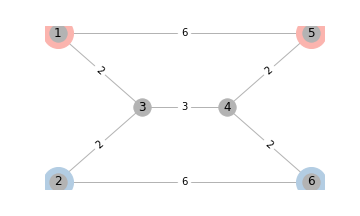
\includegraphics[width=6cm]{../resources/example_1_base.png}
    \caption{Representación de la red utilizada para el ejemplo de aplicación de la formulación binivel. Los dos pares origen-destino se detallan con un color diferente. Cada arco tiene una etiqueta con el costo de usuario sobre la infraestructura base, es decir, la red de calles.}
    \label{fig:example1base}
  \end{figure}

  Podemos deducir rápidamente en la figura de la red (\ref{fig:example1base}) que el camino más corto para ambos pares origen-destino sobre la red de calles está compuesto de un arco con costo 6. El objetivo entonces es decidir dónde construir infraestructuras 1 tal que el costo de los caminos más cortos de uno o ambos pares origen-destino sea menor a 4 (dado por la función de transferencia de demanda), de manera que una cantidad $D$ o $2D$ de demanda total pueda ser transferida a la bicicleta, nótese que los valores posibles de demanda transferida en este caso solo pueden ser $0$, $D$ y $2D$. Si decidimos utilizar infraestructura 1 en alguno de los arcos (1, 5) o (2, 6), digamos el primero, entonces nos aseguramos que la demanda del par origen-destino (1, 5) será transferida a la bicicleta, ya que el costo del camino más corto pasa a ser $3$. Con el presupuesto remanente de valor $5$, solo podremos construir infraestructura 1 en a lo sumo dos de los arcos (2, 3), (3, 4) y (4, 5). No es difícil ver que a lo sumo podremos mejorar el costo del camino más corto a $4.5$ para el par origen-destino (2, 6). La demanda transferida total en este caso es entonces de $D$.

  La solución óptima viene de construir infraestructura 1 en todos los arcos del grafo menos los (1, 5) y (2, 6). Esto permite que ambos pares origen-destino tengan un nuevo recorrido como camino más corto, de costo $3.5$, lo que permite, según la función de transferencia de demanda, transferir $2D$ unidades de demanda. Esta solución se puede observar gráficamente en la figura (\ref{fig:example1solution}).

  \begin{figure}[h!]
    \centering
    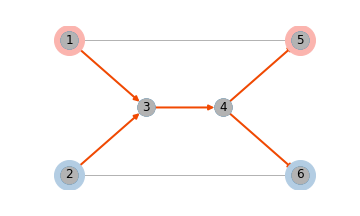
\includegraphics[width=6cm]{../resources/example_1_infras.png}
    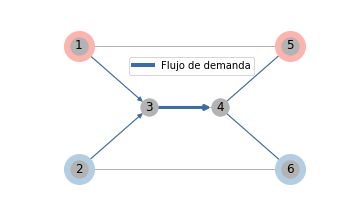
\includegraphics[width=6cm]{../resources/example_1_flows.png}
    \caption{Representación de la solución óptima en el grafo. A la izquierda se muestra en naranja en cuáles arcos se construye la infraestructura 1. A la derecha, en azul, los flujos sobre los caminos más cortos para ambos pares origen-destino. Nótese que el ancho del arco en este caso da una noción de la cantidad flujo.}
    \label{fig:example1solution}
  \end{figure}

  Para mostrar que la solución es óptima para la formulación binivel podemos decir que no hay asignación de infraestructuras a arcos que induzcan una demanda transferida mayor, dados los caminos más cortos encontrados para cada par origen-destino, para cada otra asignación posible analizada.

 \FloatBarrier
 \subsection{Hipótesis}

  En este trabajo asumimos las siguientes hipótesis que entendemos tienen sentido en este contexto:

  \begin{itemize}
    \item{El tiempo de viaje en todo arco de la red es independiente del flujo sobre el mismo.}
    \item{Existen diferentes pares origen-destino en la red, cada uno con un valor de demanda, y para cada par existen potencialmente diferentes caminos que unen el origen y el destino.}
    \item{Los usuarios siempre buscan minimizar el costo de su viaje (todos son
    perfectos optimizadores y se comportan igual)}
  \end{itemize}

  Sobre la red, consideramos que los grafos son dirigidos y cuando se decide construir una infraestructura sobre un arco solo se hace en la dirección del mismo. Esto simplifica el modelado pero puede no ser tan realista considerando que el costo marginal de construir una infraestructura, dado que existe la misma infraestructura en el otro sentido, es menor al costo de construir la primera. También puede resultar en que dados dos nodos mutuamente adyacentes, se decida construir diferentes infraestructuras en cada sentido. Sin embargo, dado que en general las redes que modelan las ciudades sobre las que se quieren resolver estos problemas son una simplificación de la red de calles, las consideraciones irreales mencionadas no tienen consecuencia práctica.

  \subsection{Características de una solución}
  \label{sect:solutioncharacteristics}

  Como marco para para evaluar la validez del modelo definimos algunas características deseables que, entendemos, deben cumplir una solución del problema cuya formulación no interesa a estos efectos.

  Consideramos que una solución cumple los siguientes puntos:

  \begin{enumerate}
      \item{El costo de los caminos más cortos entre pares origen-destino sobre la red resultante, es decir, adicionando infraestructuras, es menor o igual al costo sobre la red sin infraestructuras.}
    \item{\label{budgetexcess} El presupuesto excedente no es suficiente para agregar una infraestructura que mejore el costo de alguno de los caminos más cortos.}
    \item{El camino más corto sobre la red resultante para un par origen-destino no puede inducir un valor de demanda transferida distinto al de la solución.}
  \end{enumerate}

  \subsection{Formulación matemática}

  Finalmente presentamos la formulación matemática formal. Sean:

  \begin{description}
    \item[$OD$]: Conjunto de pares origen-destino con elemento genérico $k$. Un par origen-destino representa demanda que se traslada de un punto a otro de la red.
    \item[$G=(N,A)$]: Grafo dirigido que modela la red, con su conjunto de nodos $N$ y de arcos $A$. $A_n^+$ y $A_n^-$ son los conjuntos de arcos que salen y entran respectivamente desde el nodo $n$.
    \item[$I$]: Conjunto índice de infraestructuras de ciclovías, numeradas desde $0$ en adelante. A mayor valor mejor es la infraestructura para el usuario, es decir tiene menor costo de usuario y mayor el costo de construcción.
    \item[$C_{ai}$]: Costo de usuario de atravesar el arco $a \in A$ utilizando la infraestructura $i \in I$. $C_{ai} > 0$.
    \item[$H_{ai}$]: Costo de construcción de la infraestructura $i \in I$ sobre el arco $a \in A$. $H_{ai} \geq 0$ .
    \item[$B$]: Presupuesto para la construcción de infraestructuras.
    \item[$\theta_{nk}$]: Parámetro que vale 1 si $n$ es el origen del par origen-destino $k \in OD$, -1 si es el destino y 0 en otro caso.
    \item[$w_k$]: Variable de primer nivel que contiene el valor del camino más corto para el par origen-destino $k \in OD$ una vez que se impactan las decisiones dadas por $y_{ai}$.
    \item[$y_{ai}$]: Variable binaria de primer nivel que determina si la infraestructura $i \in I$ está activa, es decir construida, en el arco $a \in A$.
    \item[$x_{ak}$]: Variable de segundo nivel que determina si el arco $a \in A$ es parte del camino más corto para el par origen-destino $k \in OD$.
    \item[$f_k$]: Función que determina la demanda que utiliza la bicicleta como modo de transporte en función del costo del camino mas corto.
  \end{description}

  Definimos la siguiente formulación de programación matemática:

  \begin{align}
    \text{max}    & \sum_{k \in OD} f_k(w_k)                                                         & \label{eq:objective1lvl} \\
    \text{s.t.}\; & w_k = \sum_{a \in A} \sum_{k \in OD} \sum_{i \in I} C_{ai}y_{ai}x_{ak}           & \forall k \in OD \label{eq:shortestpath} \\
                  & B \geq \sum_{a \in A} \sum_{i \in I} H_{ai}y_{ai}                                & \label{eq:respectbudget} \\
                  & 1 = \sum_{i \in I} y_{ai}                                                        & \forall a \in A \label{eq:alwaysoney} \\
                  & w_k \geq 0, y_{ai} \in \{0,1\}                                                   & \nonumber \\
                  & \text{min} \sum_{a \in A} \sum_{k \in OD} \sum_{i \in I} C_{ai}y_{ai}x_{ak}      & \label{eq:subproblem} \\
                  & \text{s.t.} \sum_{a \in A_n^+} x_{ak} - \sum_{a \in A_n^-} x_{ak} = \theta_{nk}  & \forall n \in N, k \in OD \label{eq:flowbalance} \\
                  & \modelspace x_{ak} \geq 0                                                        & \nonumber
  \end{align}

  Donde:

  \begin{description}
    \item[(\ref{eq:objective1lvl})]: Función objetivo de nivel superior es la suma de los valores de demandas que cambian de modo de transporte.
    \item[(\ref{eq:shortestpath})]: Restricción que determina el costo del camino más corto dado en el primer nivel, utilizada solamente para mejor visualización.
    \item[(\ref{eq:respectbudget})]: Restricción de presupuesto sobre las infraestructuras sobre arcos que pueden estar activas.
    \item[(\ref{eq:alwaysoney})]: Restricción que requiere que una y solo una infraestructura esté activa en cada arco. Se discutirá sobre esto a continuación.
    \item[(\ref{eq:subproblem})]: Función objetivo del segundo nivel. Resuelven el problema del camino más corto para cada par origen-destino.
    \item[(\ref{eq:flowbalance})]: Restricción de balance de flujo.
  \end{description}

  \subsubsection*{Observaciones}

  Si bien dejamos sin definir explícitamente las funciones $f_k$ para facilitar el modelado debemos tener en cuenta que buscamos que la formulación completa sea lineal ya que buena parte de los avances en solvers se han desarrollado sobre este tipo de problemas.

  En la formulación del problema de primer nivel, la restricción (\ref{eq:alwaysoney}) pudo haber sido escrita de manera que a lo sumo una infraestructura esté activa, es decir, dejar la posibilidad de que no haya infraestructuras activas en un arco. Esto se puede ver de diferentes maneras. Pensando en la realidad modelada, un ciclista podría circular prácticamente por cualquier, entonces para que las instancias de la formulación (\ref{eq:objective1lvl})-(\ref{eq:flowbalance}) sean semánticamente correctas debería existir una infraestructura $i_0 \in I$ cuyo costo de construcción $H_{ai_0}$ sea 0 en todos de los arcos $a \in A$, mas allá de que el costo de usuario pueda ser arbitrariamente alto. Desde un punto de vista formal, si no se requiere que en cada arco haya siempre una infraestructura activa, se complejiza la formulación al representar de dos maneras los costos de usuario: por un lado el costo de usuario de circular por la calle que es siempre permitido y por otro el costo de circular por una de las infraestructuras especializadas si está activa.

  Por otro lado si permitimos circular solo por infraestructura especializada, deberíamos agregar al problema de segundo nivel una restricción que evite flujos en arcos donde no hay infraestructura activa, es decir: $x_{ak} \leq \sum_{i \in I} y_{ai}, \forall a \in A, k \in OD$. Con esta restricción, el problema de segundo nivel puede no tener solución factible cuando las infraestructuras seleccionadas por el primer nivel no induzcan un subgrafo que conecta todos los pares origen-destino, cosa que no es deseable desde el punto de vista de la validez del modelo binivel, ver demostraciones en el apéndice \ref{sect:apendixbilevelvalidation}, página \pageref{sect:apendixbilevelvalidation}.

  Asumiremos de aquí en adelante que las instancias del problema están bien definidas, esto significa que:

  \begin{enumerate}
    \item {$G$ es conexo}
    \item {$\forall k \in OD$ existe un camino $S_k \in G$ con costo de construcción cero, es decir $\sum_{a \in S_k} H_{ai_0} = 0$}
  \end{enumerate}

  \subsection{Consideraciones semánticas}

  Son de nuestro particular interés para la formulación los parámetros que representan la demanda y funciones de transferencia de demanda entre modos. Incurrimos en una simplificación que reduce varios modos de transporte (por ejemplo transporte público, taxi o privado) a uno, y consideramos la transferencia desde este modo agregado a la bicicleta. Otra forma de verlo es que estas funciones modelen el cubrimiento de la demanda que utilizaría la bicicleta dado el costo del camino más corto y cierto estado de la red del ciclovías, indistintamente de cuál es el modo de transporte que utilizan los usuarios al momento. Por lo tanto las funciones de transferencia de demanda son funciones de $\mathbb{R}^+$ en $\mathbb{R}^+$, cuyo dominio está en unidad del costo de usuario y su codominio en unidad de demanda que se transfiere de un modo a otro.

  \subsubsection*{Transferencia de demanda}

  El modelo busca determinar la mayor transferencia de demanda entre dos modos de transporte. Para esto, consideramos que sobre la infraestructura base la demanda transferida es cero, es decir, que el costo del camino más corto utilizando la bicicleta únicamente sobre la infraestructura base no induce transferencia de demanda. Suponemos que partimos de un conjunto de demanda insatisfecha por la infraestructura de ciclovías base, pero potencial, si las condiciones mejoran.

  En la práctica, la decisión de utilizar la bicicleta es multifactorial y depende altamente de tres tipos de factores \cite{ortuz2011}:

  % Modeling Transport, Ortuzar 2011. Pag. 208
  \begin{enumerate}
    \item{
        Características del viajante
          \begin{itemize}
            \item{Edad}
            \item{Nivel socio-económico}
            \item{Otros factores como utilización de auto para el trabajo, llevar niños a la escuela, etc.}
          \end{itemize}
    }
    \item{
        Características del viaje
          \begin{itemize}
            \item{Propósito}
            \item{Momento del día}
          \end{itemize}
    }
    \item{
        Características cuantitativas y cualitativas de las facilidades de transporte
        \begin{itemize}
            \item{Disponibilidad de transporte público}
            \item{Infraestructuras de ciclovías}
            \item{Costo de boleto y combustibles}
            \item{Comodidad y conveniencia}
            \item{Seguridad y protección}
        \end{itemize}
    }
  \end{enumerate}

  En este trabajo nos concentramos en el último punto exclusivamente. Mediante la construcción de ciclovías se podrán obtener mejoras en varios de estos puntos que modelamos como un único valor. Sobre los otros factores, asumimos que solo consideramos el universo de demanda que es transferible a la bicicleta, esto nos ahorra considerar aspectos como si el viaje se hace de noche o si el trabajo requiere un vehículo automotor.

  \section{Resolución del problema}

  Si bien la formulación binivel expresa de buena manera lo que queremos resolver, en la práctica los problemas de programación lineal binivel, o BLPP de sus siglas en inglés, son en general de difícil resolución. Ya se ha demostrado en \cite{bardbook} que el BLPP lineal en su formulación general es NP-Hard. Además, los métodos existentes para su transformación a formulaciones de un nivel no son directos. En el apéndice (\ref{sec:kkttransform}) mencionamos la metodología más común pero con cierto costo analítico que consiste en sustituir el problema del segundo nivel por las condiciones de optimalidad de Karush-Kuhn-Tucker. En este trabajo tomamos un camino alternativo reescribiendo la formulación binivel como un nivel basado en sus características estructurales y en los valores que tienen sentido para sus parámetros. Previo a esta reestructura debemos adaptar la formulación binivel de manera que las variables de diferentes niveles no se encuentren en un producto, ya que esto deviene en restricciones no lineales luego de las transformaciones.

  \subsection{Quitando producto de variables $x_{ak}$ e $y_{ai}$}

  Proponemos la siguiente formulación del problema de segundo nivel:

  \begin{align}
    \text{min}  & \sum_{k \in K} \sum_{a \in A} C_{ai} x_{ak}         & \label{eq:subproblemrefeq1} \\
    \text{s.t.} & \sum_{a \in A_n^+} x_{ak} - \sum_{a \in A_n^-} x_{ak} = \theta_{nk} & \forall n \in N, k \in OD \\
                & 0 \leq h_{aki} \leq y_{ai}                                          & \forall a \in A, k \in K, i \in I \\
                & x_{ak} = \sum_{i \in I} h_{aki}                                     & \forall a \in A, k \in K \label{eq:subproblemrefeq4}
  \end{align}

  Si utilizamos la ecuación (\ref{eq:subproblemrefeq1}) en la restricción de igualdad de $w_k$ del problema binivel (ecuación (\ref{eq:shortestpath})) entonces el problema es equivalente con la ventaja eliminamos el producto en cuestión. La equivalencia se da porque formulación (\ref{eq:subproblemrefeq1})-(\ref{eq:subproblemrefeq4}) desagrega los flujos para cada infraestructura además de para cada par origen-destino y arco en la variable $h_{aki}$, que es lo que se modela con el producto $y_{ai} x_{ak}$.

  \subsection{Formulación alternativa de un nivel}
  \label{altOneLevelFormulation}

  A diferencia de la transformación a un nivel mediante las restricciones de KKT, que podemos decir que resulta en una formulación equivalente a la binivel, en esta sección proponemos una formulación alternativa que entendemos equivalente en el sentido de lo que queremos resolver y obtener de la resolución, es decir, un valor de demanda transferida y un conjunto de decisiones de cuales infraestructuras construir y dónde.

  Esta formulación nace de la formulación binivel quitando el subproblema y agregando sus restricciones al problema de primer nivel bajo el argumento de que las funciones $f_k$ deben ser decrecientes para que el problema tenga sentido semánticamente ya que a mayor costo de usuario menor debería ser la demanda transferida. Entonces para maximizar el objetivo de nuestro problema: $\sum_{j \in OD}f_k(w_k)$, lo mejor es los $w_k$ sean lo más chico posible.

  La formulación resultante es la siguiente:

  \begin{align}
    \text{max}    & \sum_{k \in OD} f_k(w_k)                                                         & \label{eq:objectivealt} \\
    \text{s.t.}\; & w_k = \sum_{a \in A} \sum_{k \in OD} \sum_{i \in I} C_{ai}y_{ai}x_{ak}           & \forall k \in OD \label{eq:shortestpathalt} \\
                  & B \geq \sum_{a \in A} \sum_{i \in I} H_{ai}y_{ai}                                & \label{eq:respectbudgetalt} \\
                  & 1 = \sum_{i \in I} y_{ai}                                                        & \forall a \in A \label{eq:alwaysoneyalt} \\
                  & \sum_{a \in A_n^+} x_{ak} - \sum_{a \in A_n^-} x_{ak} = \theta_{nk}              & \forall n \in N, k \in OD \label{eq:flowbalancealt} \\
                  & w_k \geq 0, x_{ak} \geq 0, y_{ai} \in \{0,1\}                                    & \nonumber
  \end{align}

  \subsubsection*{Observaciones}

  La formulación en realidad asume que las funciones $f_k$ son estrictamente decrecientes. Si las funciones son solo decrecientes, entonces puede haber valores de costos de caminos más cortos que no tienen incentivo a decrecer.
  % Tuve que sacar un comentario sobre que no imponemos que las funciones sean decrecientes porque mas abajo en la validación se utiliza que son estrictamente.

  \subsection{Definición de las $f_k$s}

  Lo que resta definir es cómo modelamos las funciones $f_k$. Nuestro objetivo es definir un mecanismo para que cualquier tipo de función pueda ser expresada como un problema de optimización lineal y que este se pueda acoplar a la formulación existente.

  Podemos encontrar en la literatura soluciones a problemas similares. En Laporte 2007 \cite{laporte2007} y Lim 2021 \cite{lim2021}, se considera un parámetro $c^{PRIV}_k$ que modela el costo del transporte privado para un par origen-destino $k$, si la red de transporte público logra un costo menor, entonces se considera que toda la demanda del par origen-destino $k$ se transfiere a dicho modo, lo que se conoce como {\it all-or-nothing}.

  \subsubsection{Definición propuesta}

  Consideramos que una función $f_k$ arbitraria debe poder modelar una transición paulatina de la demanda entre modos de transporte cuya curva puede comportarse de diferentes formas como analizamos en secciones posteriores. Asumiendo que las $f_k$ son decrecientes, el enfoque que seguimos es representarla como una sucesión decreciente de puntos de quiebre, tal que para cada uno exista un valor asociado de cantidad de demanda transferida. Su representación gráfica sería una función escalonada donde cada escalón es constante, ver figura (\ref{fig:fdrawexample}). Al evaluar una función, los puntos de quiebre son comparados contra el valor del camino más corto $w_k$ seleccionando el mínimo valor mayor a $w_k$. Entonces sea $w_k$ fijo, la demanda transferida es:

  \begin{equation}
    \label{eq:deffks}
    f_k(w_k) = P_{j^*},\; j^* = argmin_{j \in J} \{Q_j \geq w_k\}
  \end{equation}

  Donde $Q_j$ son los puntos de quiebre en la unidad del costo del camino más corto, $J$ es un conjunto índice y $P_{j^*}$ es la cantidad de demanda que se transfiere.

  Una ventaja de esta formulación es que puede ser integrada a la función objetivo de la formulación de nuestro problema (\ref{eq:objectivealt})-(\ref{eq:flowbalancealt}), de manera que la minimización queda en manos del objetivo del mismo problema.

  Para modelar la función $argmin$ en una formulación como la que venimos trabajando es necesario utilizar variables de activación que permitan que sólo un valor del conjunto índice esté activo (para cada $k$). Por ejemplo, si se usa $z_j,\; j \in J$, lo antedicho equivale a decir que $z_j \in \{0,1\}$ y $\sum_{j \in J} z_j = 1$. Luego queda en manos de la minimización elegir el $z_j$ activo óptimo.

  Nótese que esta definición es una extensión de la {\it all-or-nothing}. Para modelarla basta considerar $J = \{0, 1\}$, $P_0 = 0, P_1 = D_k$ y $Q_0 = M, Q_1 = c^{PRIV}_k$, donde $M$ es un número arbitrario mayor a $c^{PRIV}_k$ y $D_k$ es la demanda para el par origen-destino $k$.

  \begin{figure}[h!]
    \centering
    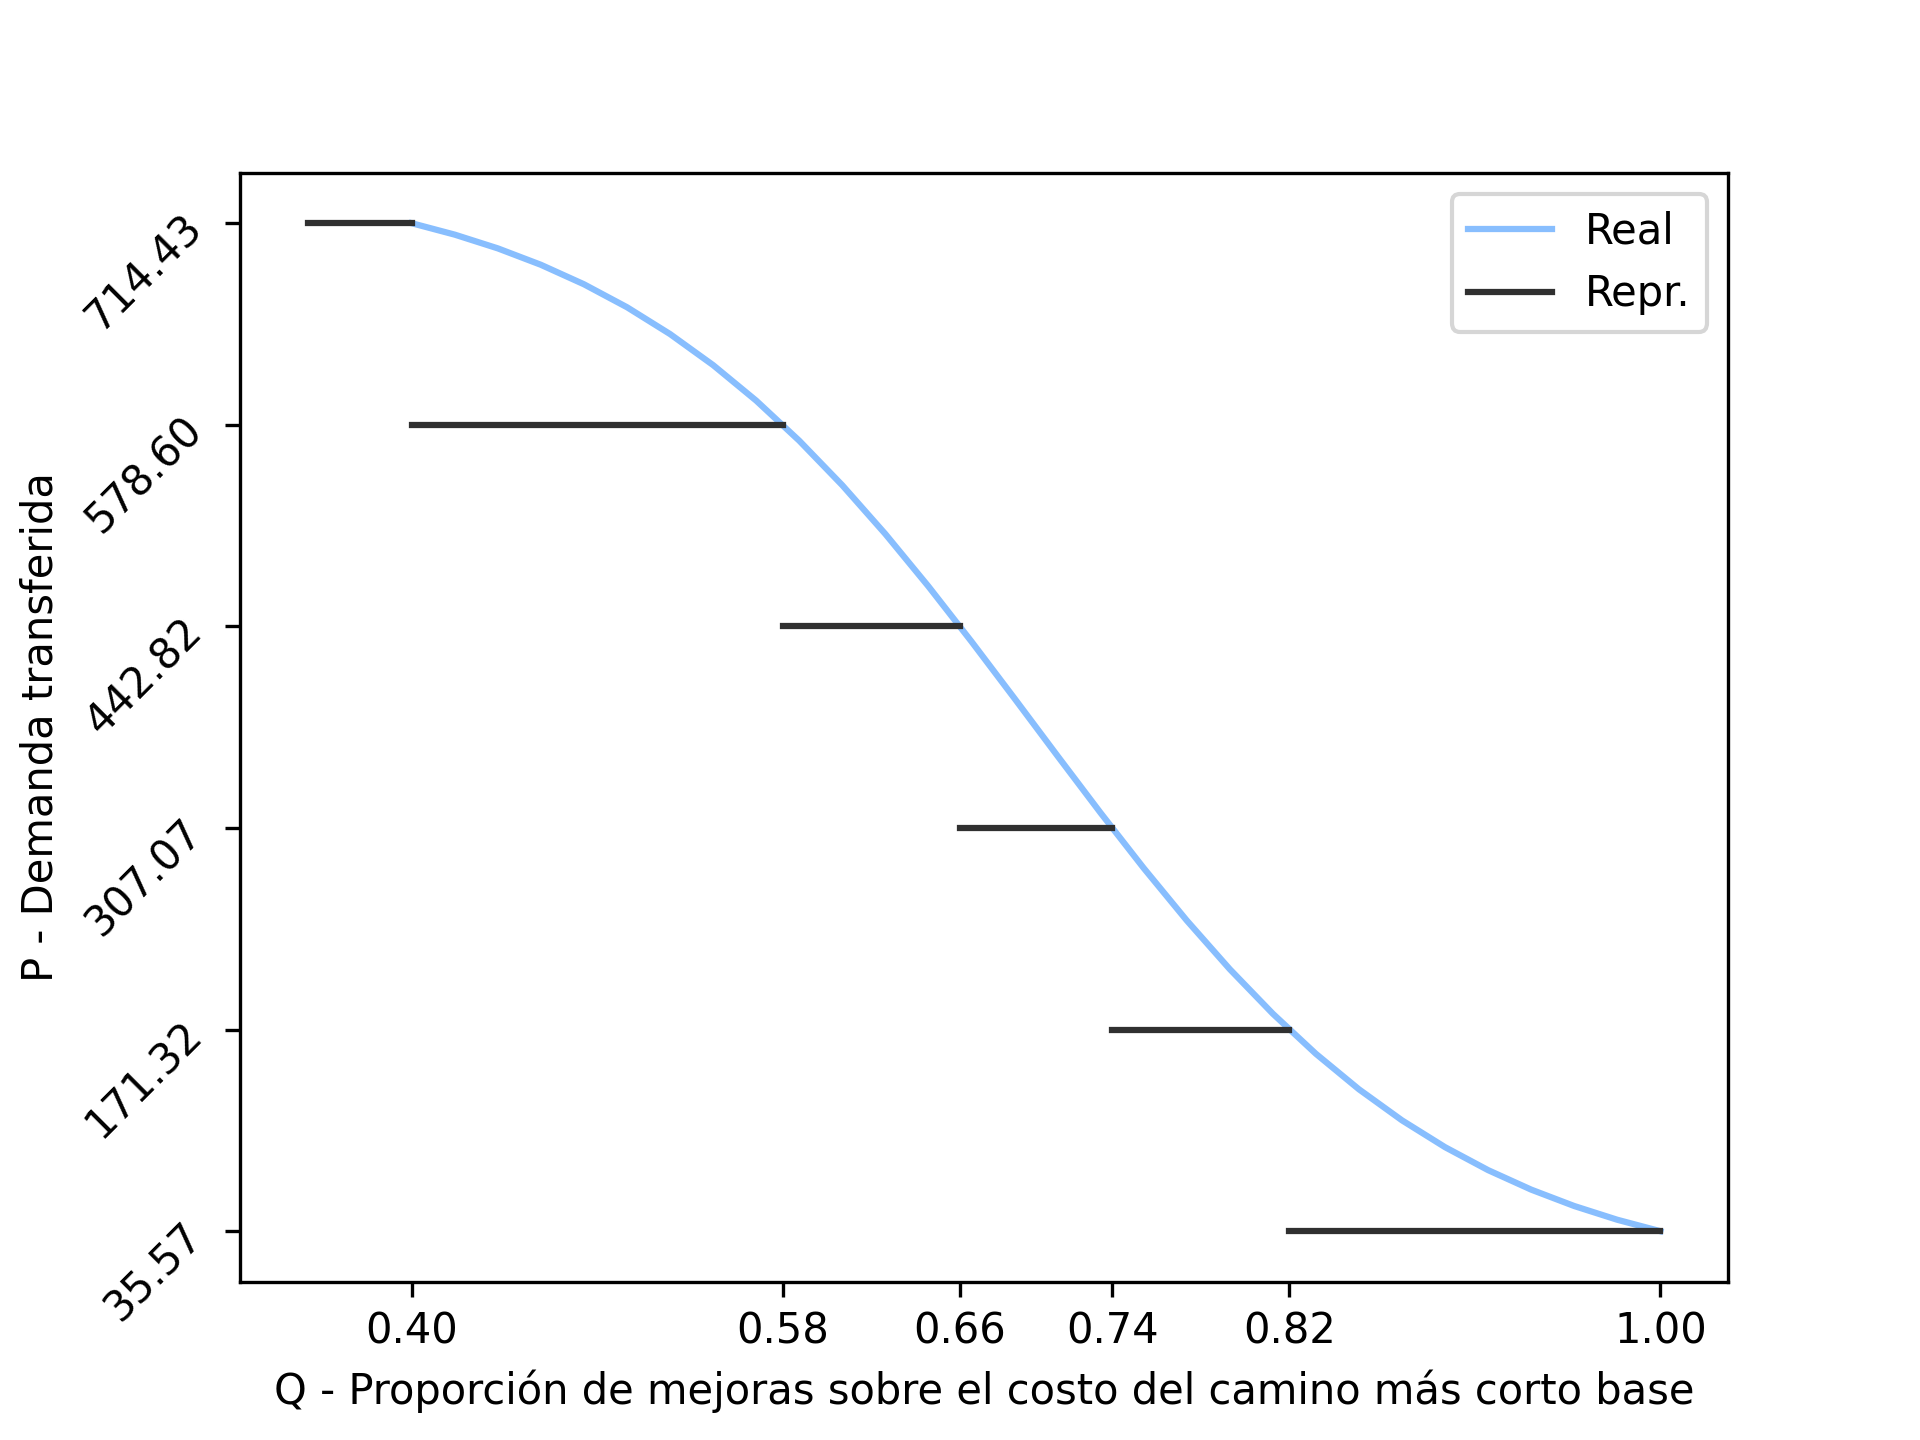
\includegraphics[width=8cm]{../resources/f_example.png}
    \caption{Ejemplo de una función arbitraria y su representación con el mecanismo planteado. Los puntos donde hacer los quiebres son arbitrarios.}
    \label{fig:fdrawexample}
  \end{figure}

  \FloatBarrier
  \subsubsection{Formulación de $f_k$ como LP}

  La forma más simple de modelar $f_k$ (ó simplemente $f$) es la (\ref{eq:fkv1eq1})-(\ref{eq:fkv1eq4}). Sea $W \in \mathbb{R}^+$ un valor del costo de un camino:

  \begin{align}
    f(W) =\; & max \sum_{j \in J} P_j y_j    & \label{eq:fkv1eq1}\\
             & s.t. \sum_{j \in J} y_j = 1   & \label{eq:fkv1eq2} \\
             & \;\;\; Q_j \geq W y_j         & \label{eq:fkv1eq3} \forall j \in J \\
             & \;\;\; y_j \in \{0,1\}        & \label{eq:fkv1eq4} \forall j \in J
  \end{align}


  La definición anterior es un problema lineal bien formulado, sin embargo no puede ser integrada tal cual está a la formulación (\ref{eq:objectivealt}) - (\ref{eq:flowbalancealt}) sin perder linealidad dado que $W$ es modelado con variable ($w_k$) entonces el resultado seria un problema no lineal por la restricción (\ref{eq:fkv1eq3}). Por este motivo estudiamos dos formulaciones alternativas que logran solucionar esta situación. La idea en ambas es desagregar $W$ como la suma de nuevas variables y utilizar estas en la restricción (\ref{eq:fkv1eq3}) en lugar del producto $W y_j$.

  \paragraph*{$f_k$ como LP versión 1}

  \begin{align}
    f(W) =\; & max \sum_{j \in J} P_j y_j             & \label{eq:fkv3eq1}\\
             & s.t. \sum_{j \in J} y_j = 1            & \label{eq:fkv3eq2}\\
             & \;\;\; Q_j \geq w^{aux}_j              & \forall j \in J \label{eq:fkv3eq3} \\
             & \;\;\; w^{aux}_j \leq M y_j            & \forall j \in J \label{eq:fkv3eq4} \\
             & \;\;\; w^{sink}_j \leq M (1 - y_j)     & \forall j \in J \label{eq:fkv3eq5} \\
             & \;\;\; w^{sink}_j + w^{aux}_j = W      & \label{eq:fkv3eq6} \forall j \in J\\
             & \;\;\; y_j \in \{0,1\}                 & \label{eq:fkv3domainy} \forall j \in J \\
             & \;\;\; w^{aux}_j, w^{sink}_j \geq 0    & \label{eq:fkv3eq7} \forall j \in J
  \end{align}

  Se desagrega $W$ para cada $j$ en $w^{sink}_j + w^{aux}_j$ de manera que uno de los dos tenga el valor de $W$, esto se logra con las restricciones (\ref{eq:fkv3eq4}) y (\ref{eq:fkv3eq5}). Entonces se cumple que solo el $w^{aux}_j$ cuyo $y_j$ esté activo tendrá el valor de $W$, mientras que para el resto de los $j$ las variables $w^{sink}_j$ habrán tomado dicho valor. Las mencionadas restricciones sirven para activar $y_i$ y utilizan un parámetro $M \geq W$ arbitrario. Finalmente, las restricciones (\ref{eq:fkv3eq2}) y (\ref{eq:fkv3eq6}) logran que solo una de las variables $w^{aux}_j$ o $w^{sink}_j$ tome el valor de $W$, para cada $j$.

  \paragraph*{$f_k$ como LP versión 2}

  \begin{align}
    f(W) =\; & max \sum_{j \in J} P_j y_j             & \label{eq:fkv2eq1}\\
             & s.t. \sum_{j \in J} y_j = 1            & \label{eq:fkv2eq2}\\
             & \;\;\; Q_j \geq w^{aux}_j              & \forall j \in J \label{eq:implfkoriginalineq} \\
             & \;\;\; w^{aux}_j \leq M y_j            & \forall j \in J \label{eq:yactivation1} \\
             & \;\;\; \sum_{j \in J} w^{aux}_j = W    & \label{eq:activatewaux} \\
             & \;\;\; y_j \in \{0,1\}                 & \label{eq:fkv2domainy} \forall j \in J\\
             & \;\;\; w^{aux}_j \geq 0                & \label{eq:fkv2eq6} \forall j \in J
  \end{align}

  En este caso se desagrega $W$ como suma de $|J|$ variables $w^{aux}_j$ de manera que solo una de ellas esté activa y tenga el valor de $W$. Para activar $y_j$ se agrega la restricción (\ref{eq:yactivation1}) utilizando, igual que en la formulación anterior, un parámetro $M \geq W$. Finalmente las restricciones (\ref{eq:activatewaux}) y (\ref{eq:fkv2eq2}) logran que solo uno de los $w^{aux}_j$ tome el valor de $W$ y el resto sean 0.

  \subsubsection{Validación de la formulación}

  Según definimos $f_k(W)$ en la fórmula (\ref{eq:deffks}), sea $p = f_k(W)$, entonces se cumple que:

  \begin{enumerate}
    \item {\label{deffpt1} $p$ es exactamente uno de los valores del conjunto de valores $P_j$, es decir: $p \in \{P_j\}_{j \in J}$}
    \item {\label{deffpt2} Sea $\hat{j} = j \;|\; p = P_j$. Se cumple que el valor del punto de quiebre $Q$ asociado a $\hat{j}$ no es menor que el costo del camino más corto $W$, es decir: $Q_{\hat{j}} \geq W$.}
    \item {\label{deffpt3} Dado el $\hat{j}$ anterior, entonces no existe un punto de quiebre $Q_j \forall j \in J\setminus\{\hat{j}\}$ que sea no mayor al punto de quiebre $Q_{\hat{j}}$ y mayor o igual al costo del camino más corto, es decir: $\not{\exists}\; Q_j\; \forall j \in J\setminus\{\hat{j}\} \;|\; Q_j \in  [W, Q_{\hat{j}}]$}.
  \end{enumerate}

  Es de nuestro interés analizar la correctitud de las formulaciones respecto a los puntos mencionados.

  Para la versión 1, tenemos que el punto \ref{deffpt1} se cumple en la función objetivo donde el valor objetivo es la suma sobre el conjunto $\{P_j\}_{j \in J}$, la restricción (\ref{eq:fkv3eq2}) dice que solo uno de esos valores puede estar activo en la suma del objetivo dado el dominio de la variable $y_j$. Luego, el punto \ref{deffpt2} se cumple dado que $y_{\hat{j}} = 1$ por el punto anterior, entonces $w_{\hat{j}}^{aux} = W$ por restricciones (\ref{eq:fkv3eq4}), (\ref{eq:fkv3eq5}) y (\ref{eq:fkv3eq6}) y la restricción (\ref{eq:fkv3eq3}) verifica el punto en cuestión. Finalmente, el punto \ref{deffpt3} se cumple por el hecho de que la función objetivo es una maximización y que $f(W)$ es una función estrictamente decreciente, entonces, si existiera un $Q_a \in \{Q_j\}_{j \in J} \;|\; Q_a < Q_{\hat{j}}, a \in J$, existe un valor $P_a > P_{\hat{j}}$ lo que contradice el hecho de que el objetivo sea una maximización.

  Podemos utilizar las justificaciones de los puntos 1 y 3 para la versión 2 de la formulación. Luego, el punto \ref{deffpt2} se cumple dado que $y_{\hat{j}} = 1$ por las los puntos anteriores y junto a que que $w^{aux}_{\hat{j}} = W$ por las restricciones (\ref{eq:fkv2eq2}), (\ref{eq:yactivation1}) y (\ref{eq:activatewaux}) tenemos que la condición se cumple en la restricción (\ref{eq:implfkoriginalineq}).

  \subsubsection{Valores posibles de $P_j$ y $Q_j$}

  Los valores que tienen sentido para los conjuntos $Q$ y $P$ son cualquier subconjunto discreto del dominio de la función de transferencia de demanda y su valor funcional, respectivamente. Dado un par origen-destino $k \in OD$ entendemos que tiene sentido que el dominio de $f_k$ sean valores de costos del camino más corto entre el mejor posible y el peor. Dada una instancia del problema y un par origen destino, llamamos $\underline{W}$ al costo del camino más corto suponiendo que las mejores infraestructuras se pueden construir y $\overline{W}$ al costo del camino más corto sobre el grafo base (sin infraestructuras especiales) \footnote{En realidad, $\overline{W}$ es el mínimo valor para el que $f_k$ es mínimo, podría ser cualquier número arbitrariamente grande.}, entonces $Q_j \in [\underline{W}, \overline{W}],\; \forall j \in J$. Los valores de $Pj$ son la cantidad de demanda que se transfiere para cada $Q_j$, es decir $P = \{f_k(Q_j):\; j \in J\}$. El conjunto índice $J$ determina la precisión con que se representa la función $f_k$.

  Es deseable también que el mínimo de $f_k$ sea 0 y que el máximo sea la demanda total del par $k$: $D_k$, osea $f_k(\overline{W}) = 0$ y $f_k(\underline{W}) = D_k$. Es decir, si ninguna mejora es impuesta al camino más corto no haya transferencia de demanda así como si la mejor infraestructura posible es construida toda la demanda se transfiera. Esto tiene sentido si trabajamos solamente con la demanda transferible a la bicicleta, dejando afuera la que ya utiliza dicho medio de transporte, la que en ningún caso la utilizaría y la que requiere de costos de usuario demasiado bajos para las posibilidades de la instancia.

  Una forma posible de establecer los valores de $J$, $P_j$ y $Q_J$ es: dada una función $f_k$, tomando $N$ valores equidistantes entre $[\underline{W}, \overline{W}]$ obtendremos $Q_j$ y tomando el valor funcional de esos puntos obtendremos $P_j$, luego $J=\{1,..,N\}$.

  \subsection{Poniendo todo junto}
  \label{sect:alltogether}

  Luego del análisis hecho, ensamblamos la formulación final de manera explícita. Dado que tenemos dos variantes del modelado de las $f_k$ entonces también tendremos dos variantes de esta formulación. Aquí presentamos la formulación completa utilizando la versión 2 de $f_k$, siendo la otra muy similar. Fundamentalmente sobre estas dos variantes trabajamos en lo que sigue.

  Además de las definiciones en la formulación inicial (\ref{eq:objective1lvl})-(\ref{eq:flowbalance}), agregamos las siguientes:

  \begin{description}
    \item[$J$]: Conjunto índice utilizado en los conjuntos $P$ y $Q$.
    \item[$P_{kj}$]: Parámetro que determina la cantidad de demanda transferida para el par origen-destino $k \in OD$ y el índice $j \in J$.
    \item[$Q_{kj}$]: Parámetro que contiene el punto de quiebre para determinar la demanda transferida para el par origen-destino $k \in OD$ e índice $j \in J$.
    \item[$M$]: Número positivo muy grande.
    \item[$z_{kj}$]: Variable binaria que determina si la demanda transferida para el par origen-destino $k \in OD$ es la de índice $j \in J$.
    \item[$h_{aki}$]: Variable no negativa que determina el flujo que pasa por el arco $a \in A$, para el par origen-destino $k \in OD$ utilizando la infraestructura $i \in I$.
    \item[$w^{aux}_{kj}$]: Variable no negativa que contiene el valor de $w_{k}$ si $z_{kj}$ esta activa y de lo contrario cero.
  \end{description}

  \begin{align}
    \text{max}    & \sum_{k \in OD} \sum_{j \in J} P_{kj} z_{kj}                          & \label{eq:objectivefinalalt} \\
    \text{s.t.}\; & w_k = \sum_{a \in A} \sum_{i \in I} C_{ai}h_{aki}                     & \forall k \in OD \label{eq:shortestpathaltfinal} \\
                  & Q_{kj} \geq w^{aux}_{kj}                                              & \forall j \in J, k \in OD \label{eq:breakpointsalt} \\
                  & w^{aux}_{kj} \leq M z_{kj}                                            & \forall j \in J, k \in OD \\
                  & \sum_{j \in J} w^{aux}_{kj} = w_k                                     & \forall k \in OD \\
                  & \sum_{j \in J} z_{kj} = 1                                             & \forall k \in OD \label{eq:singularbreakpointalt} \\
                  & B \geq \sum_{a \in A} \sum_{i \in I} H_{ai}y_{ai}                     & \label{eq:respectbudgetaltfinal} \\
                  & 1 = \sum_{i \in I} y_{ai}                                             & \forall a \in A \label{eq:alwaysoneyaltfinal} \\
                  & \sum_{a \in A_n^+} x_{ak} - \sum_{a \in A_n^-} x_{ak} = \theta_{nk}   & \forall n \in N, k \in OD \label{eq:flowbalancealtfinal} \\
                  & x_{ak} = \sum_{i \in I} h_{aki}                                       & \forall a \in A, k \in K \label{eq:flowactivationalt} \\
                  & 0 \leq h_{aki} \leq y_{ai}                                            & \forall a \in A, k \in K, i \in I \label{eq:respectinfraalt} \\
                  & z_{kj} \in \{0,1\}                                                    & \nonumber \\
                  & w_k \geq 0, y_{ai} \in \{0,1\}, x_{ak} \geq 0, h_{aki} \geq 0         & \nonumber
  \end{align}

  Donde las nuevas ecuaciones son:

  \begin{description}
    \item[\ref{eq:objectivefinalalt}]: Función que suma los valores de demanda transferida $P_{kj}$ activos.
    \item[\ref{eq:breakpointsalt}]: Restricción que determina que los puntos de quiebre activos son aquellos cuyo costo es menor o igual al del camino más corto.
    \item[\ref{eq:singularbreakpointalt}]: Restricción que permite solo un punto de quiebre activo para cada par origen-destino $k \in OD$.
    \item[\ref{eq:flowactivationalt}]: El flujo total para el arco $a \in A$ y el par origen-destino $k \in OD$ es la suma de los flujos de todos las infraestructuras.
    \item[\ref{eq:respectinfraalt}]: El flujo por el arco $a \in A$, para el par origen-destino $k \in OD$ y la infraestructura $i \in I$ puede estar activo si la infraestructura $i$ esta activa.
  \end{description}

  \subsection{Validación}

  En esta sección analizamos las dos variantes de la formulación de un nivel (\ref{eq:objectivefinalalt})-(\ref{eq:respectinfraalt}) con pequeñas variantes adicionales y mostramos su validez de manera experimental.

  Como mecanismo de validación, utilizamos las características deseables de una solución mencionadas al principio en la sección \ref{sect:solutioncharacteristics}, página \pageref{sect:solutioncharacteristics}. Comprobando dichos puntos sobre las soluciones obtenidas por las formulaciones estudiadas podemos tener confianza de que ellas resuelven lo deseado. También fueron de utilidad para detectar bugs durante el desarrollo.

  \subsubsection{Variantes de la formulación}

  Durante la implementación y pruebas preliminares de la formulación (\ref{eq:objectivefinalalt})-(\ref{eq:respectinfraalt}) observamos que en algunos casos los flujos no eran consistentes con la hipótesis del comportamiento de los usuarios, es decir, no iba por el camino más corto entre origen y destino. La fundamentación es que las funciones $f_k$ son constantes entre dos valores consecutivos de $Q_{kj}$ lo cual causa que en dicho dominio no exista incentivo para optimizar el costo del camino más corto.

  Para contrarrestar esto consideramos dos opciones, que en definitiva cambian nuestra formulación monoobjetivo a una multiobjetivo. Llamémosle subobjetivo al sumando que agregaremos a la función objetivo (\ref{eq:objectivefinalalt}).

  En la primera opción agregamos variables de holgura $r_{kj} \geq 0$ que modelan la diferencia entre el punto de quiebre $Q_{kj}$ activo y el costo del camino más corto $w_k$ para un par origen-destino. Dichas variables también son agregadas a la función objetivo.
  Esto cambia a nivel del modelado de las funciones $f_k$ la ecuación (\ref{eq:breakpointsalt}) que queda de esta manera:

  \begin{equation}
    \label{eq:multipleobj1breakpoint}
    Q_{kj} z_{kj} - r_{kj} = w^{aux}_{kj}
  \end{equation}

  Advertir que esta restricción se encuentra en ambas versiones de la formulaciónes de $f_k$ por lo tanto en ambos casos se aplica esta variante.

  Sea el parámetro $\beta > 0$, la función multiobjetivo 1 es:

  \begin{equation}
    \label{eq:multipleobj1}
    \sum_{k \in OD} \sum_{j \in J} \left( P_{kj}z_{kj} + \beta r_{kj} \right)
  \end{equation}

  Otra forma de abordar esta situación es vincular los objetivos de los problemas de primer y segundo nivel en (\ref{eq:objective1lvl})-(\ref{eq:flowbalance}). Dado que los dos objetivos optimizan en direcciones contrarias entonces el coeficiente del subobjetivo que originalmente era una minimización debería ser un valor negativo. Sea el parámetro $\rho > 0$, entonces podemos expresar el multiobjetivo 2 como:

  \begin{equation}
    \label{eq:multipleobj2}
    \sum_{k \in OD} \left[ -\rho w_k + \sum_{j \in J} P_{jk}z_{kj} \right]
  \end{equation}

  Notar que al modificar el objetivo del problema estamos, estrictamente hablando, solucionando otro problema. Sin embargo a los efectos prácticos podemos en este caso encontrar valores de los pesos relativos de cada subobjetivo de manera de que se resuelva correctamente nuestro problema y se pueda calcular la demanda transferida total con posterioridad a la resolución. Dicho de otra manera, para cada peso $\beta$ y $\rho$ existe un intervalo $[0, \beta_{max}]$ y $[0, \rho_{max}]$ respectivamente, en el que el valor computado de demanda transferida es igual. Intuitivamente lo que tiene que suceder es que el valor del subobjetivo sea intrascendente respecto a los saltos posibles en los puntos de quiebre para cada par origen destino lo que permite que ambos objetivos puedan comportarse de manera independiente. Entendemos sin embargo, que este enfoque puede traer problemas numéricos dependiendo de los valores de cada instancia.

  Otra desventaja de modificar el objetivo, en particular en problemas MIP con instancias difíciles, es que perdemos capacidad de interpretación del MIP GAP, o distancia relativa de la mejor solución factible a la mejor cota encontradas por el solver hasta cierto punto de la ejecución del algorítmico Branch and Bound.

  \subsubsection{Ejemplo - Beneficio de variantes multiobjetivo}
  \label{sect:example2}

  Este ejemplo busca ilustrar por qué es necesario agregar nuevos objetivos a la función objetivo de (\ref{eq:objectivefinalalt})-(\ref{eq:respectinfraalt}) de forma de optimizar no solo la demanda transferida, sino que también obtener una buena decisión de ubicación y tipo de infraestructuras.

  Para este ejemplo utilizaremos como base la red descrita en el cuadro (\ref{table:example2arccosts}) y en la figura (\ref{fig:example2base}). Al igual que el ejemplo presentado al principio, consideramos el costo de usuario sobre la infraestructura base y el costo de construcción de la primer infraestructura no base como el costo de los arcos que se detallan en dicha figura. Consideramos solo dos tipos de infraestructuras, la base y la infraestructura 1 que reduce el costo de usuario a la mitad; un par origen-destino, $(1, 6)$ con demanda $D$, un presupuesto de 5 y la siguiente función de transferencia de demanda:

  $$
    f(x) = \left\{ \begin{array}{lcr}
            D & \mbox{si}   & x \leq 4.5 \\
            0 & \mbox{sino} &
    \end{array}
    \right.
  $$

  \begin{table}[h!]
    \centering
      \caption*{{\bf Costo de usuario y de construcción por arco por tipo de infraestructura}}
    \begin{tabular}{cccccc}
      \toprule
      Arco & CU base & CU 1 & CC base & CC 1 & \\
      \midrule
        (1, 2) & 3 & 1.5 & 0 & 3 \\
        (1, 3) & 3 & 1.5 & 0 & 3 \\
        (1, 5) & 4 & 2   & 0 & 4 \\
        (2, 3) & 2 & 1   & 0 & 2 \\
        (2, 4) & 3 & 1.5 & 0 & 3 \\
        (3, 2) & 3 & 1.5 & 0 & 3 \\
        (3, 4) & 2 & 1   & 0 & 2 \\
        (3, 5) & 2 & 1   & 0 & 2 \\
        (4, 5) & 4 & 2   & 0 & 4 \\
        (4, 6) & 2 & 1   & 0 & 2 \\
        (5, 4) & 4 & 2   & 0 & 4 \\
        (5, 6) & 2 & 1   & 0 & 2 \\
      \bottomrule
    \end{tabular}
      \caption{Resumen de costos de usuario (CU) y de construcción (CC) para cada infraestructura.}\label{table:example2arccosts}
  \end{table}

  \begin{figure}[h!]
    \centering
    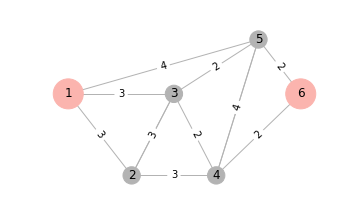
\includegraphics[width=6cm]{../resources/example_2_base.png}
      \caption{Red utilizada para el ejemplo de beneficio de variantes multiobjetivo. El camino más corto sobre el grafo base es el (1, 5), (5, 6) de costo 6.}
    \label{fig:example2base}
  \end{figure}

  \FloatBarrier

  Presentamos dos soluciones: la S utilizando monoobjetivo, y la SM utilizando cualquiera de las variantes multiobjetivo (ecuaciones (\ref{eq:multipleobj1}) ó (\ref{eq:multipleobj2})).

  La solución S, representada en la figura (\ref{fig:example2solv2}), es la siguiente:

  \begin{itemize}
    \item{Demanda transferida total: $D$}
    \item{Infraestructura de tipo 1 construida en arcos (1, 3) y (4, 6)}
    \item{Presupuesto utilizado 5}
    \item{El camino más corto es (1, 3), (3, 4), (4, 6) con costo 4.5}
  \end{itemize}

  Mientras que la solución SM, en la figura (\ref{fig:example2solv1}), es:

  \begin{itemize}
    \item{Demanda transferida total: $D$}
    \item{Infraestructura de tipo 1 construida en el arco (1, 5)}
    \item{Presupuesto utilizado 4}
    \item{El camino más corto es (1, 5), (5, 6) con costo 4}
  \end{itemize}

  Las decisiones tomadas por la versión multiobjetivo fueron mejores en términos de las infraestructuras a construir que la monoobjetivo ya que el costo de usuario resultante disminuyó en mayor cantidad y el presupuesto utilizado fue menor, aunque esto último es circunstancial. Para analizar el porqué primero debemos definir los puntos de quiebre de esta instancia. Dada la simplicidad de la función de transferencia de demanda podemos utilizar solo dos puntos de quiebre, entonces $J = \{0, 1\}$, $Q = \{6, 4.5\}$ y $P = \{0, D\}$. Omitiremos los índices $k$ del par origen-destino dado que existe uno solo. Tenemos que el $z_j$ activo, que determina el valor de demanda transferida, es aquel con $j = 1$ dado que sabemos que la demanda transferida es $D$.

  Considerando la opción multiobjetivo 1 (\ref{eq:multipleobj1}), tenemos de la restricción (\ref{eq:multipleobj1breakpoint}) que $r_1 = Q_1 - w^{aux}$ y siendo $w^{aux} = w$ por ser el punto de quiebre activo entonces $r_1 = 4.5 - w$ y el objetivo es $D + r_1$. En el caso de la solución S resulta en $r_1 = 0$ y para SM en $r_1 = 0.5$. Por lo tanto la presencia de $r_{kj}$ en el objetivo ayuda a elegir la solución SM sobre la S en este caso.

  Si utilizamos la formulación multiobjetivo 2 (\ref{eq:multipleobj2}), tenemos que el valor objetivo evaluado en la solución S es $D - 4.5$ y en la solución SM es de $D - 4$, por lo tanto la solución SM también es mejor según esta formulación.

  Vale la pena aclarar que las solución SM es, para la versión monoobjetivo, tan buena como la S. En general, asumiendo que los pesos $\beta$ y $\rho$ fueron elegidos de acuerdo a la sección anterior, las soluciones obtenidas por las versiones multiobjetivo también son soluciones óptimas de la monoobjetivo.

  Finalizamos este ejemplo comentando que ambas soluciones S y SM satisfacen los criterios definidos en las características de una solución definidas en la sección (\ref{sect:solutioncharacteristics}), página \pageref{sect:solutioncharacteristics}.

  \begin{figure}[h!]
    \centering
    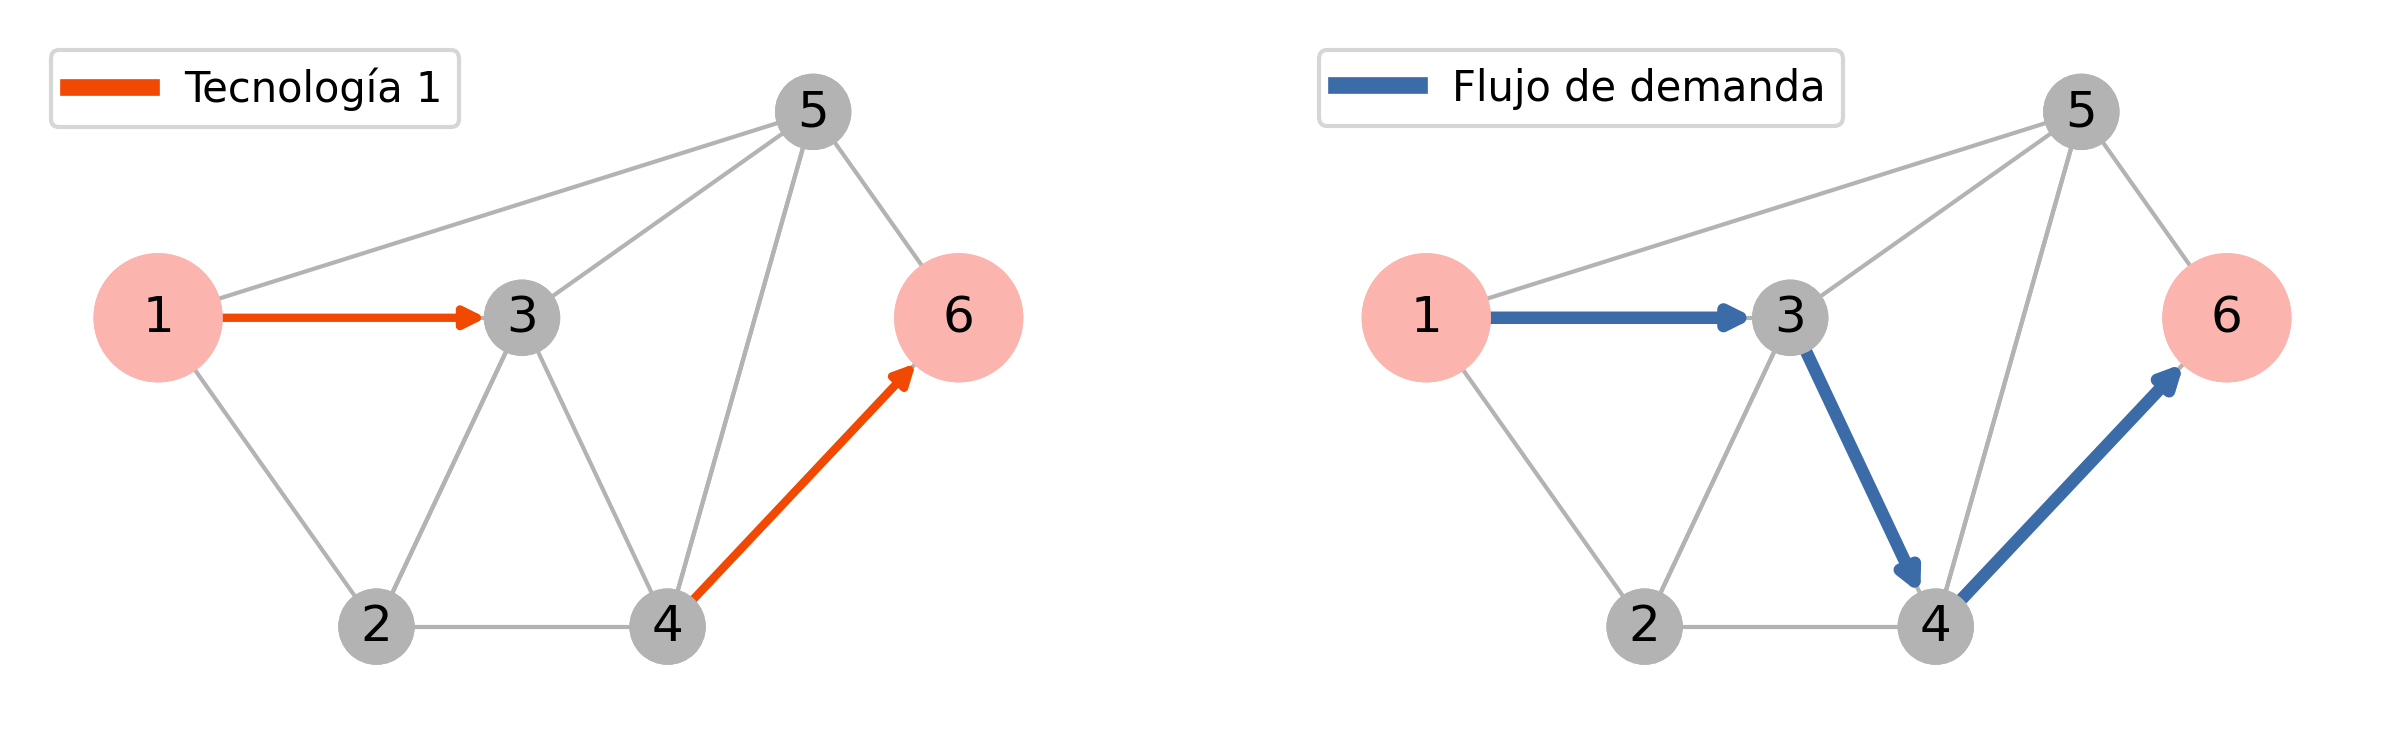
\includegraphics[width=12cm]{../resources/example_2_sol_v2.png}
      \caption{Representación de la solución S. A la izquierda se resaltan los arcos donde se construye infraestructura 1. A la derecha se observa el camino más corto sobre la red resultante.}
    \label{fig:example2solv2}
  \end{figure}

  \begin{figure}[h!]
    \centering
    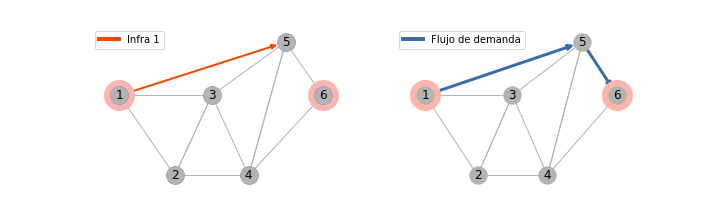
\includegraphics[width=12cm]{../resources/example_2_sol_v1.png}
      \caption{Solución SM. A la izquierda se resalta el arco donde se construye infraestructura 1 mientras que a la derecha se muestra el camino más corto, que coincide con el de la red base.}
    \label{fig:example2solv1}
  \end{figure}

  \FloatBarrier
  \subsection{Validación experimental}

  El procedimiento de validación experimental consistió en generar instancias aleatorias, solucionarlas con las diferentes versiones y verificar que se cumplan las condiciones sobre las soluciones. Las diferentes alternativas fueron sobre la formulación de un nivel, dadas por las dos implementaciones de las $f_k$, las dos versiones multiobjetivo y la versión monoobjetivo. Consideraremos en principio parámetros $\beta = 1$ y $\rho = 1$.

  Utilizamos la ciudad de Sioux-Falls como grafo base, dada su amplia adopción en literatura relativa al tema. Los datos de nodos y arcos fueron obtenidos del repositorio de instancias de redes de transporte \footnote{Transportation Networks Repositort \url{https://github.com/bstabler/TransportationNetworks}}. El costo de usuario se tomo igual al largo del arco así como el costo de construcción de la primer infraestructura no base. Consideramos en total tres tipos de infraestructuras incluyendo la base. El cálculo de costos de usuario y construcción se realizó en base a los costos de usuario base y de construcción para la infraestructura 1, como se detalla en el apéndice \ref{sect:costcalculation}, página \pageref{sect:costcalculation}.

  Se generaron entre 1 y 14 pares origen-destino y entre 2 y 10 valores de $P$ y $Q$ aleatorios cumpliendo con la hipótesis de modelar una función decreciente.
  De esta manera se generaron y probaron 1000 instancias para cada una de las seis variantes de las formulaciones. Ademas de los chequeos sobre las soluciones, fue de nuestro interés comparar los valores de demanda transferida total y tiempos de ejecución.

  \FloatBarrier
  \subsubsection{Resultados}

  \begin{table}[h!]
    \centering
    \caption*{{\bf Resumen de ejecuciones}}
    \begin{tabular}{cccccc}
      \toprule
      Versión & Versión $f_k$ & Multiobj. 1 & Multiobj. 2 & \shortstack{Cant. \\ Incump.} & \shortstack{Tiempo \\ Promedio (s)} \\
      \midrule
      v1 & v2 & Si & No & 0   & 9.34    \\
      v2 & v2 & No & No & 76  & 22.94   \\
      v3 & v1 & Si & No & 0   & 539.78  \\
      v4 & v1 & No & No & 67  & 495.80  \\
      v5 & v2 & No & Si & 0   & 11.92   \\
      v6 & v1 & No & Si & 0   & 283.93  \\
      \bottomrule
    \end{tabular}
    \caption{Comparativa agregada de ejecuciones sobre instancias aleatorias utilizando la red Sioux-Falls. Los incumplimientos de una solución fueron contados en 1 si la solución no cumplía al menos uno de los puntos. En las versiones v2 y v4 los incumplimientos detectados incumplen únicamente el punto (\ref{budgetexcess}) de las características de una solución.}\label{table:resumenejecuciones}
  \end{table}

  En las pruebas no detectamos diferencias en términos de los valores objetivos entre diferentes formulaciones a excepción de una instancia. Para la versión $v1$ y $v3$, encontramos que la presencia de variables $r_{kj}$ en el objetivo puede resultar en una solución que induce menor valor de demanda transferida total en comparación a las otras formulaciones cuando se cumple que el valor de demanda transferida para un par origen-destino $k$ es comparable a la magnitud de $r_{kj}$, para el $j$ dado que $z_{kj}$ está activa. Por ejemplo, si para un par origen-destino se puede optimizar el camino más corto de manera de transferir cierta cantidad de demanda adicional pero esto afecta la variable $r_{kj}$ de manera que la diferencia con el siguiente punto de quiebre es mayor que el nuevo salto en demanda transferida, entonces el modelo elige no realizar la mejora.

  También observamos que en las versiones v2 y v4, con optimización monoobjetivo, se ve afectada en algunos casos la validez del ítem (\ref{budgetexcess}) de la característica de una solución. Esto se explica en casos en que la construcción de una infraestructura en un arco puede mejorar el costo del camino más corto pero no lo suficiente para afectar la cantidad de demanda transferida, lo cual implica que las decisiones de qué infraestructuras construir pueda ser peor que en las otras variantes en el sentido del costo del camino más corto, como se mostró en el ejemplo (\ref{sect:example2}). En este caso sin embargo el presupuesto excedente es suficientemente para mejorar el camino de algún par origen-destino.

  A pesar de las diferencia encontrada en el valore de demanda transferida en un caso para las versiones v1 y v3, consideramos que aquellas multiobjetivo son las candidatas a ser elegidas como versión final dado que nos interesa tanto el valor objetivo como las decisiones en términos de infraestructuras. Las diferencias en los valores de demanda transferida pueden ser corregidas ajustando los pesos relativos de los objetivos.

  \begin{figure}[h!]
    \centering
    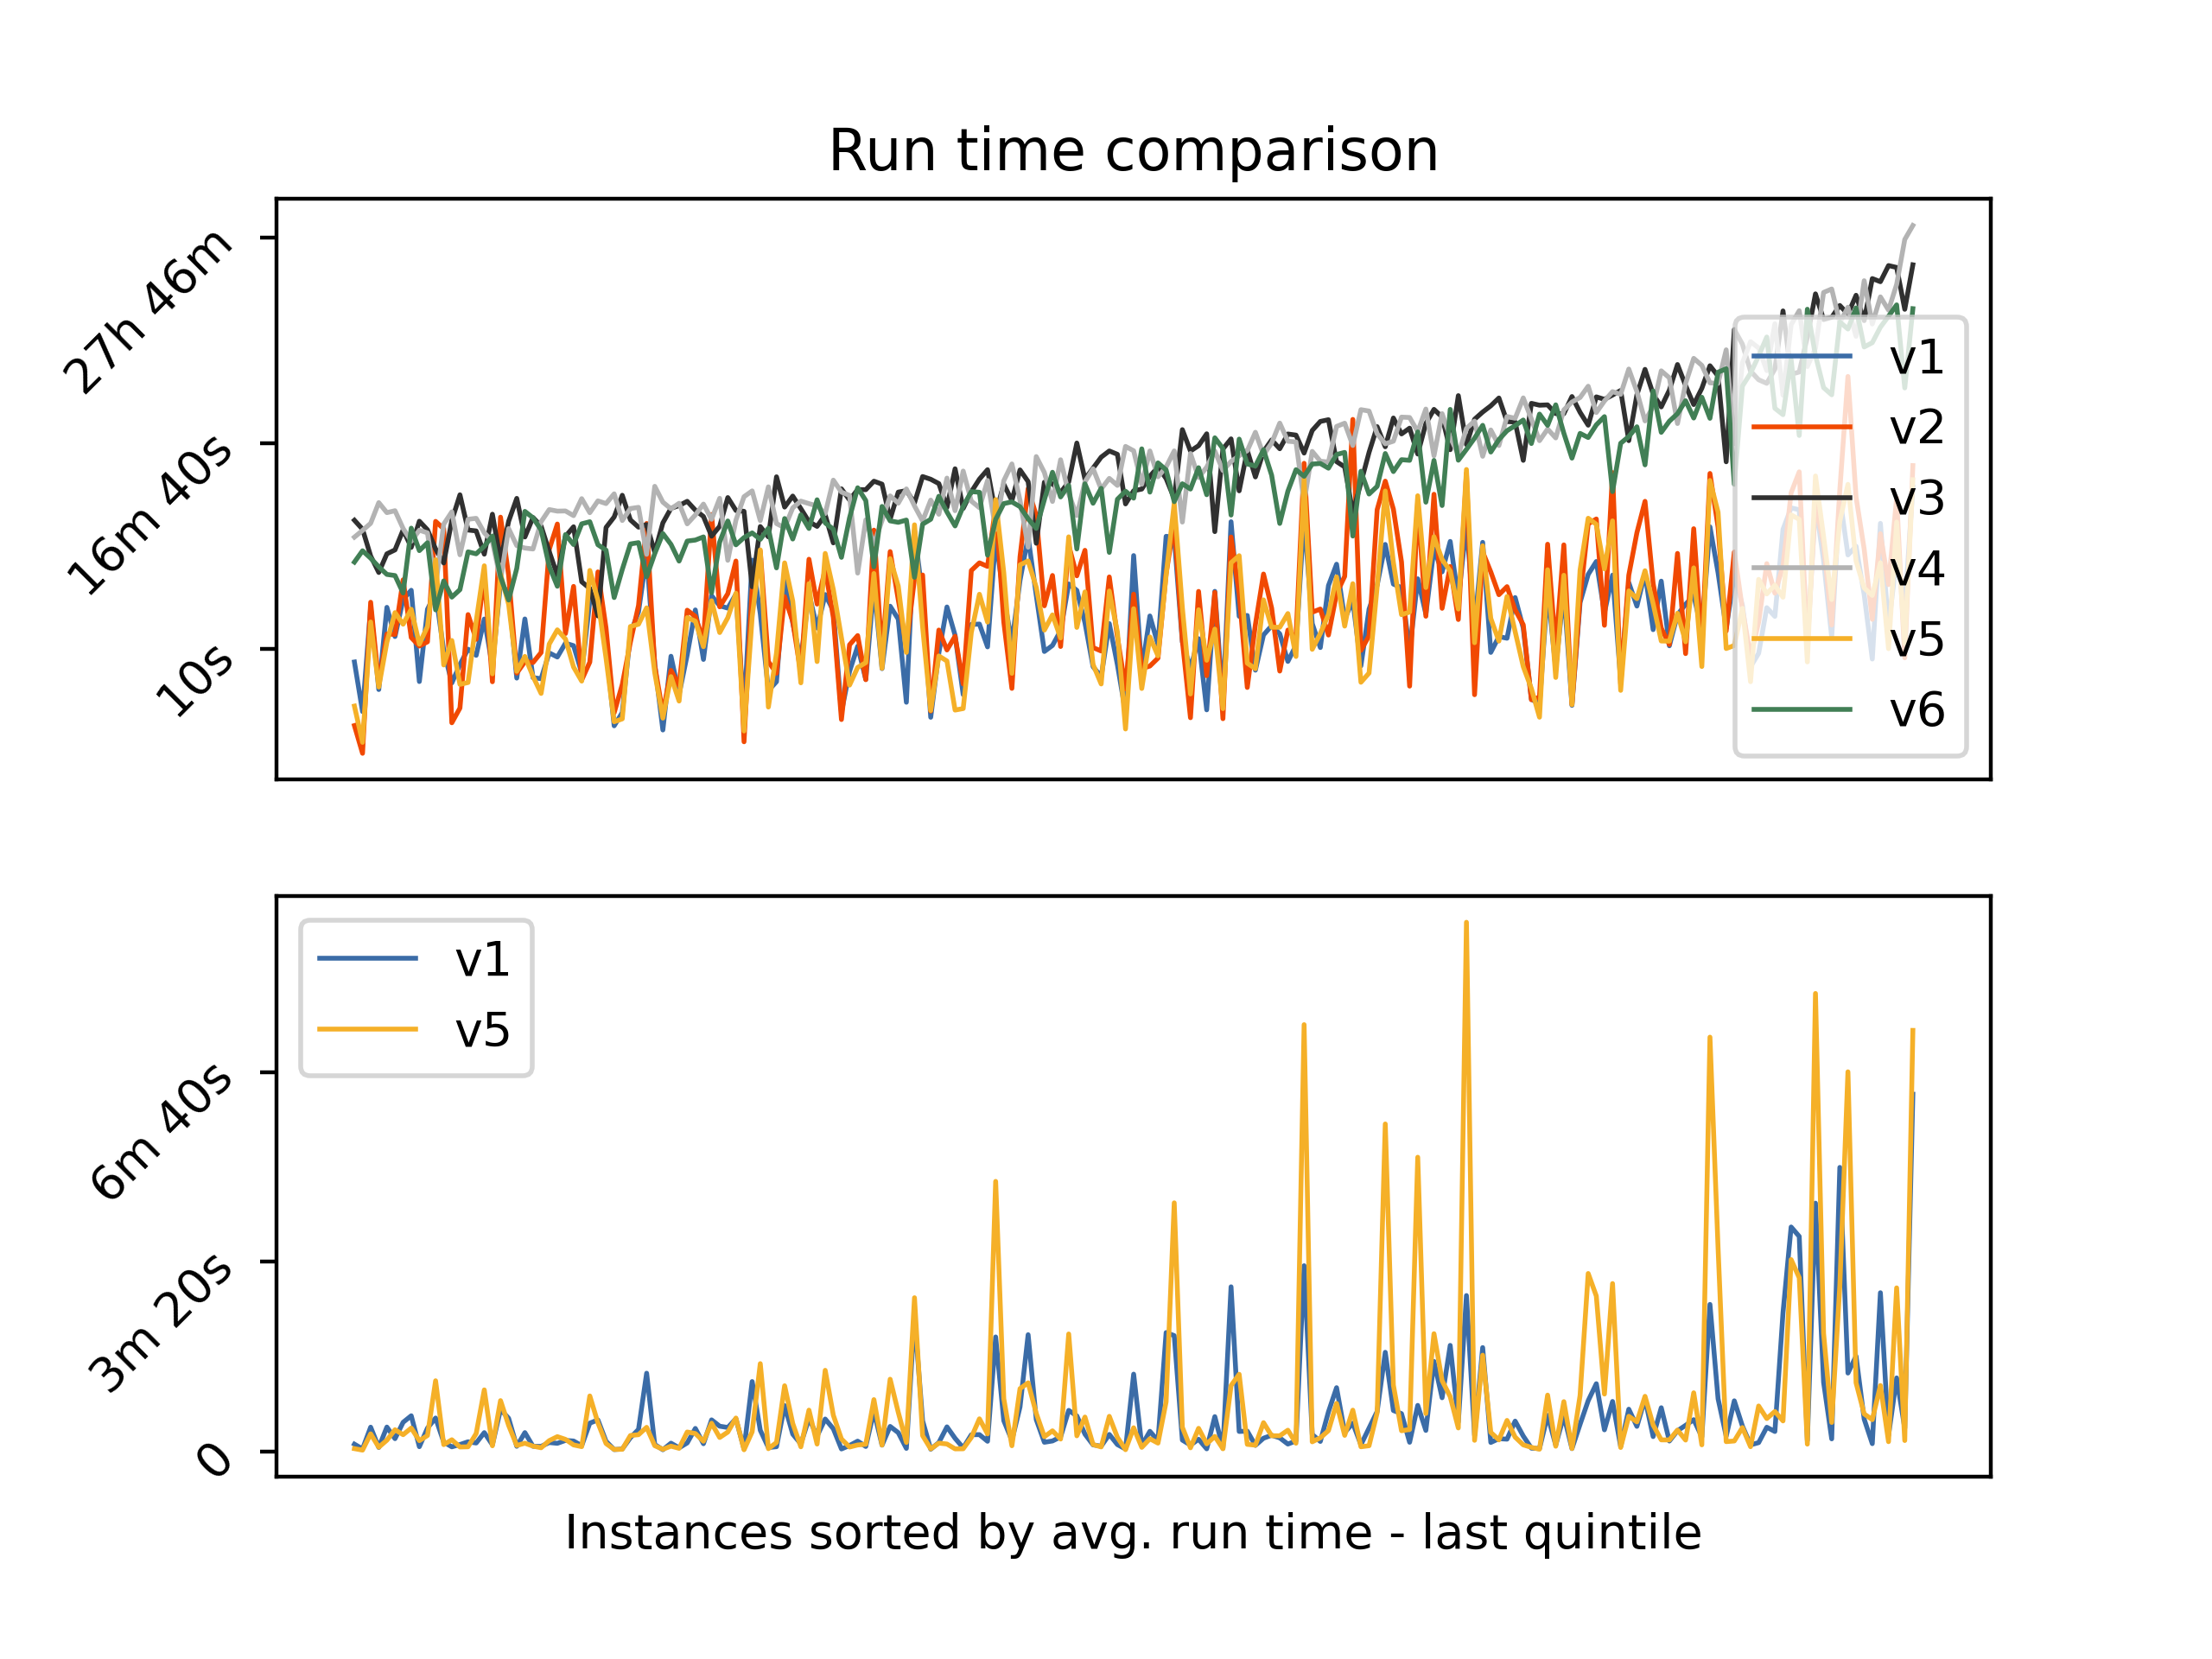
\includegraphics[width=10cm]{../resources/run_time_comparsion.png}
    \caption{Comparativa del tiempo de ejecución de todas las versiones. Las instancias, en las abscisas, fueron ordenadas de forma creciente según el tiempo promedio de ejecución de todas las versiones. En la primer gráfica, la escala es logarítmica, dado que los valores a comparar oscilan entre pocos segundos y casi treinta horas. En la segunda gráfica la escala es lineal. Tomamos las últimas 200 instancias y las dos versiones con menor tiempo de ejecución para mostrar mejor la escasa diferencia entre ellas.}
    \label{fig:runtimecomparison}
  \end{figure}

  \begin{figure}[h!]
    \centering
    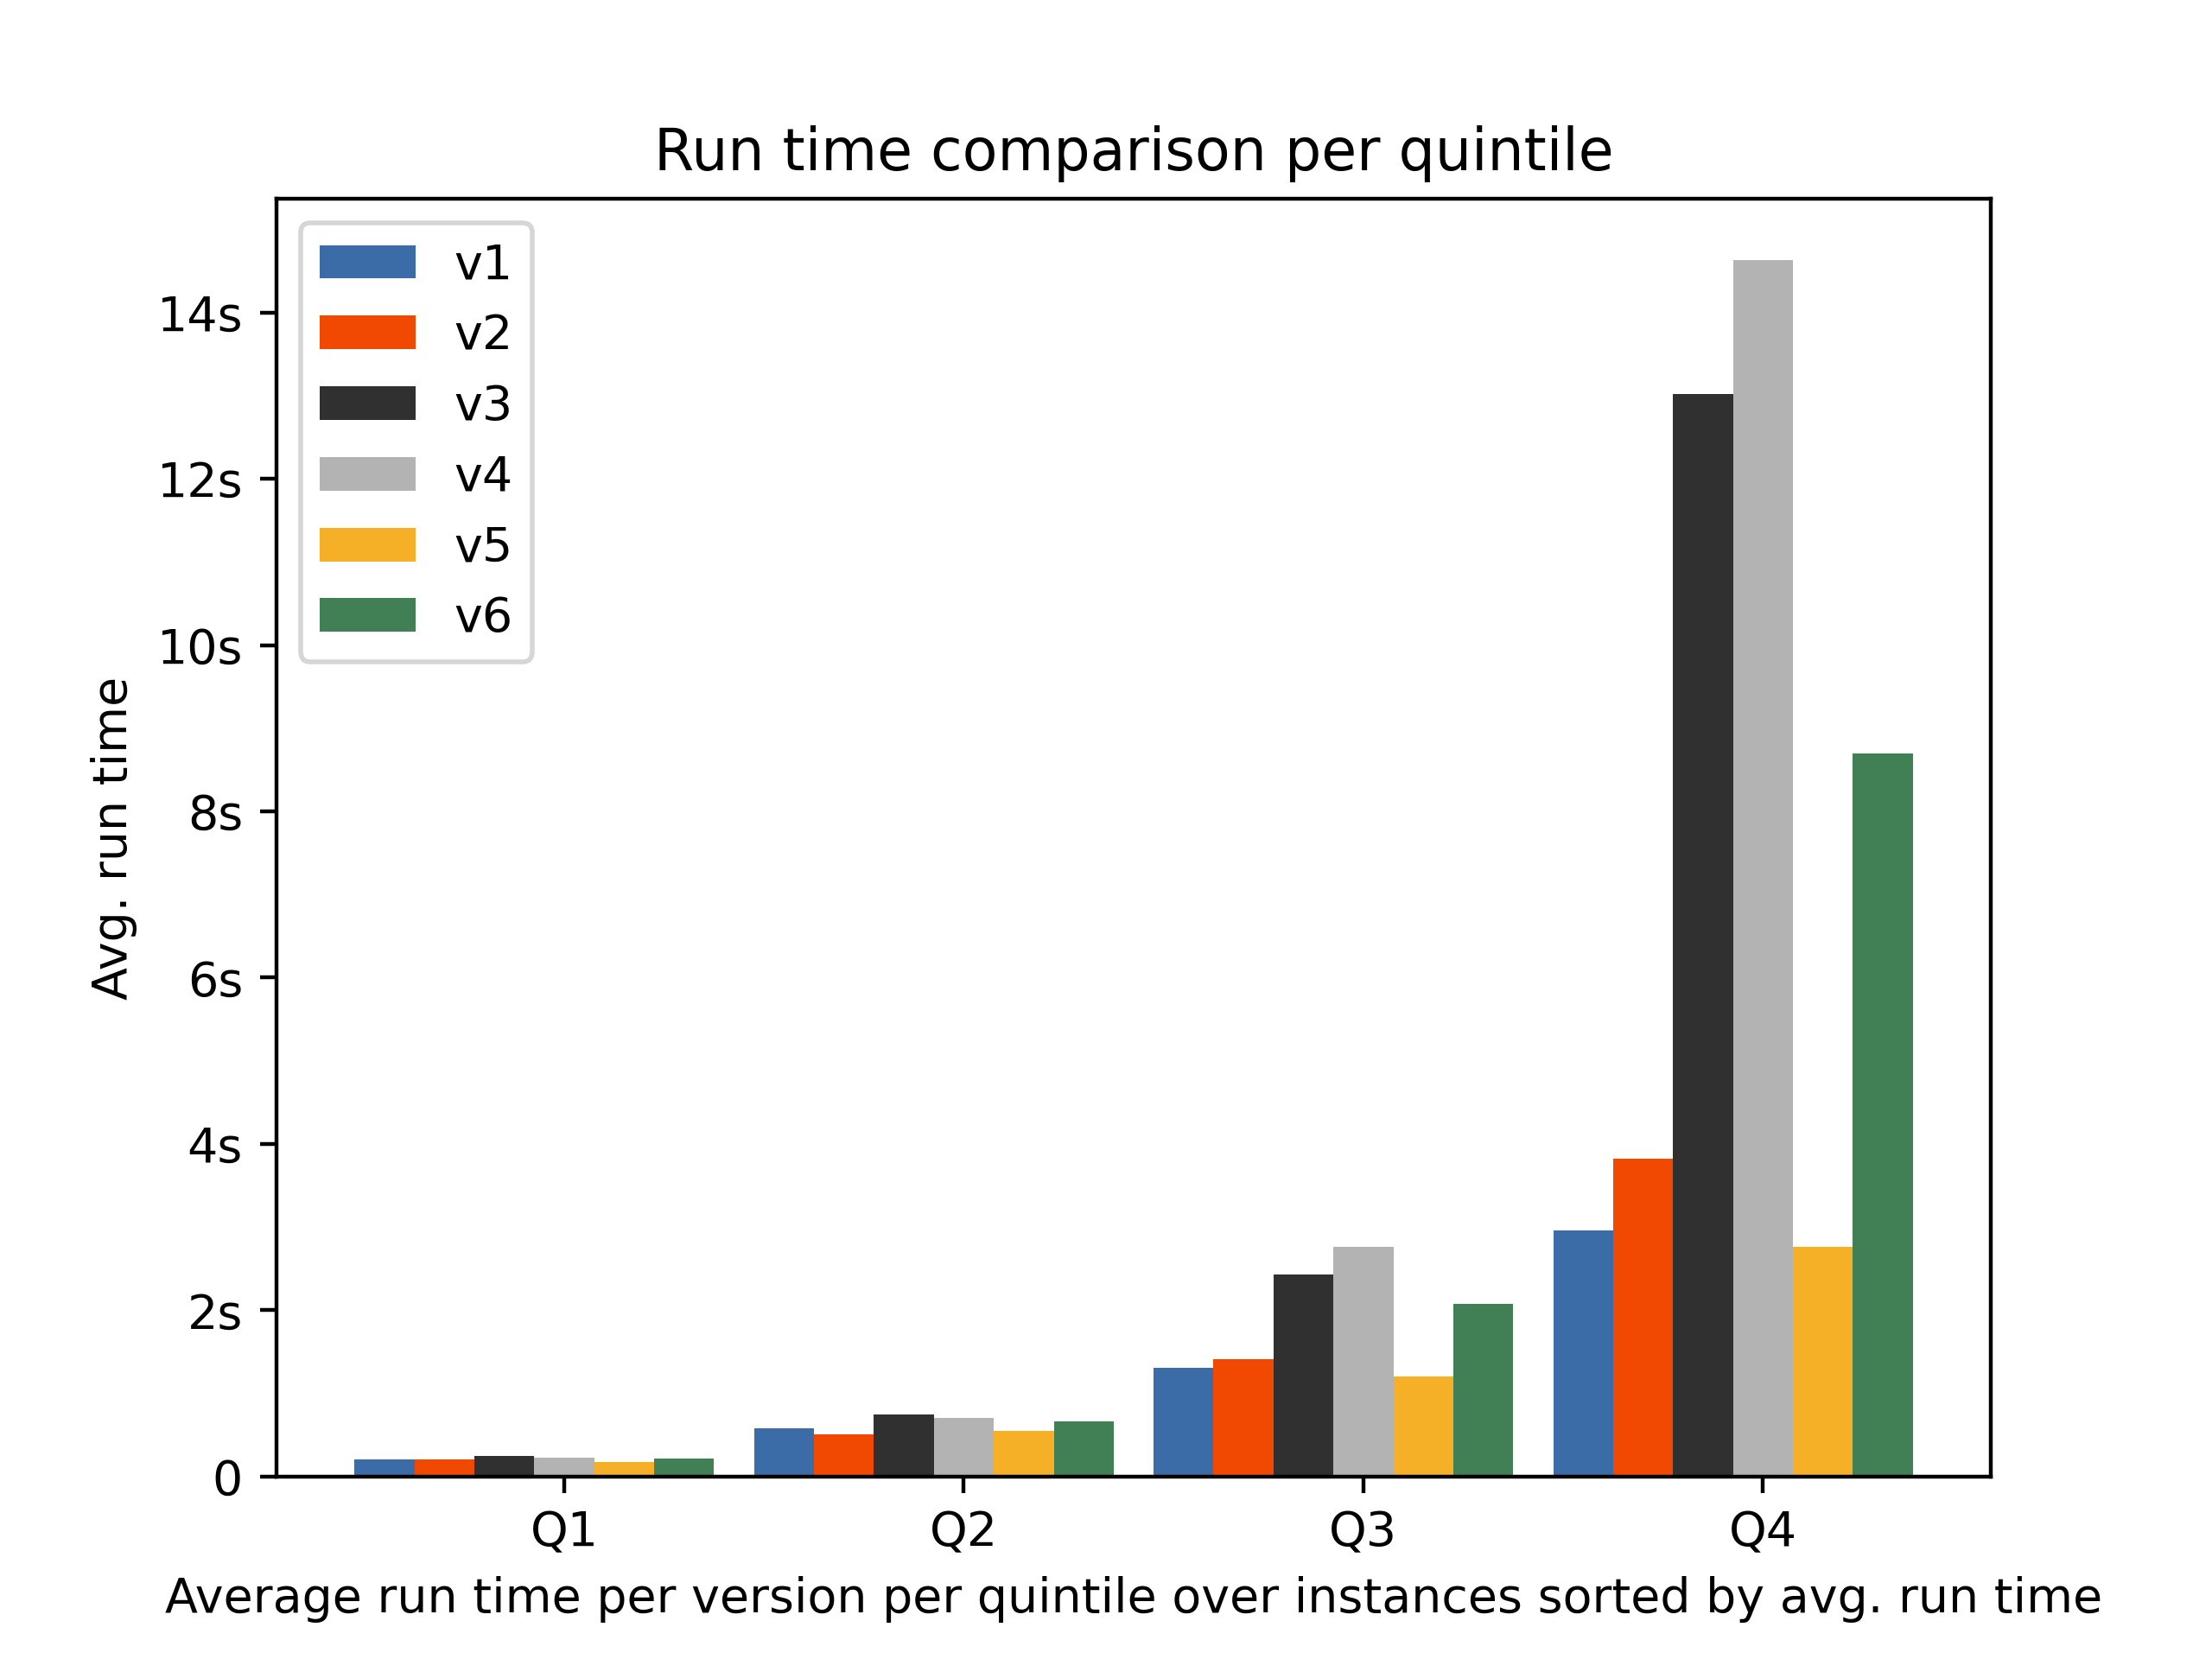
\includegraphics[width=10cm]{../resources/run_time_comparsion_by_quintile.png}
      \caption{Comparativa del tiempo de ejecución de todas las versiones en tiempo promedio para los cuatro primeros quintiles. El tiempo promedio considerado es acumulado sobre los quintiles anteriores.}
    \label{fig:firstfourquintiles}
  \end{figure}

  El siguiente aspecto que tuvimos en cuenta es el tiempo de ejecución. El tiempo de ejecución promedio nos da una medida gruesa para comparar y descartar algunas versiones, considerando que las instancias de prueba son chicas y deberían ser de fácil resolución \footnote{El ser fácil está directamente relacionado a la complejidad en tiempo.}. Las versiones v3, v4 y v6, que utilizan la formulación v1 de $f_k$ tienen un tiempo de ejecución significativamente más alto que las demás, que utilizan la otra versión. Nos interesó determinar si esta diferencia se da por algún tipo de instancia particular y si alguna versión se desempeña mejor en términos de tiempo de ejecución cuando quitamos las posibles instancias difíciles. En la figura (\ref{fig:runtimecomparison}) se puede comparar el tiempo de ejecución de las versiones en las instancias mas difíciles del conjunto de 1000 instancias generadas. Las versiones con mayor tiempo de ejecución promedio muestran una clara diferencia con las otras. También se comparan las dos versiones con menor tiempo promedio de ejecución, donde se observa que la v1 es, en la gran mayoría de los casos, la más rápida. Para las instancias mas sencillas (primeros cuatro quintiles en figura (\ref{fig:firstfourquintiles})), los tiempos de ejecución no varían demasiado entre formulaciones y solo hacia el quintil cuatro se notan algunas diferencias aunque estas son de algunos segundos.

  Considerando el tiempo de ejecución promedio y el hecho de que no hubo incumplimientos en los chequeos de las soluciones, se perfila mejor las implementaciones que utiliza la segunda versión de formulación de $f_k$ y multiobjetivo 1, es decir la formulación v1. Sin embargo, previo a la elección final, decidimos solucionar el problema que causa diferencias en el valor objetivo y realizar la comparativa nuevamente.

  Para solucionar la diferencia en demanda transferida cambiamos el valor del parámetro $\beta$ en (\ref{eq:multipleobj1}) de manera que se disminuye el efecto de las variables de $r_{kj}$ en la función objetivo de la formulación v1. El nuevo valor de $\beta$ es calculado para cada instancia y corresponde al factor mínimo entre los valores, para cada par origen-destino, que hace que el costo del camino más corto para dicho par sea menor a la menor cantidad de demanda que se transfiere de un punto de quiebre a otro. Es decir, se intenta encontrar un número que satisfaga: $\beta r_{kj} \leq min_{j \in J} \{ P_{kj} \},\; \forall r_{kj} \in [0, W_k]$.

  Se ejecutaron nuevas pruebas comparando las tres versiones mas rápidas: v1, v2 y v5. Esta se generaron 1000 nuevas instancias aleatorias con cuatro infraestructuras lo que le da mayor complejidad. Nótese que si bien la v2 tiene incumplimientos estos no implican que las soluciones sean erróneas a los efectos de la demanda transferida.

  % La versión v1 modificada sobre las instancias de la primera ronda no genero soluciones con incumplimientos y su tiempo de ejecución promedio
  % fue 10,31 segundos

  \begin{table}[h!]
    \centering
    \caption*{{\bf Resumen de ejecuciones - Segunda ronda}}
    \begin{tabular}{ccc}
      \toprule
      Versión & Cant. Incump. & T. Promedio (s) \\
      \midrule
      v1 & 0   & 79.71   \\
      v2 & 119 & 282.11  \\
      v5 & 0   & 207.50  \\
      \bottomrule
    \end{tabular}
    \caption{Comparativa agregada de ejecuciones sobre la segunda ronda de instancias aleatorias sobre la red de Sioux-Falls.}\label{table:resumenreejecuciones}
  \end{table}

  \begin{figure}[h!]
    \centering
    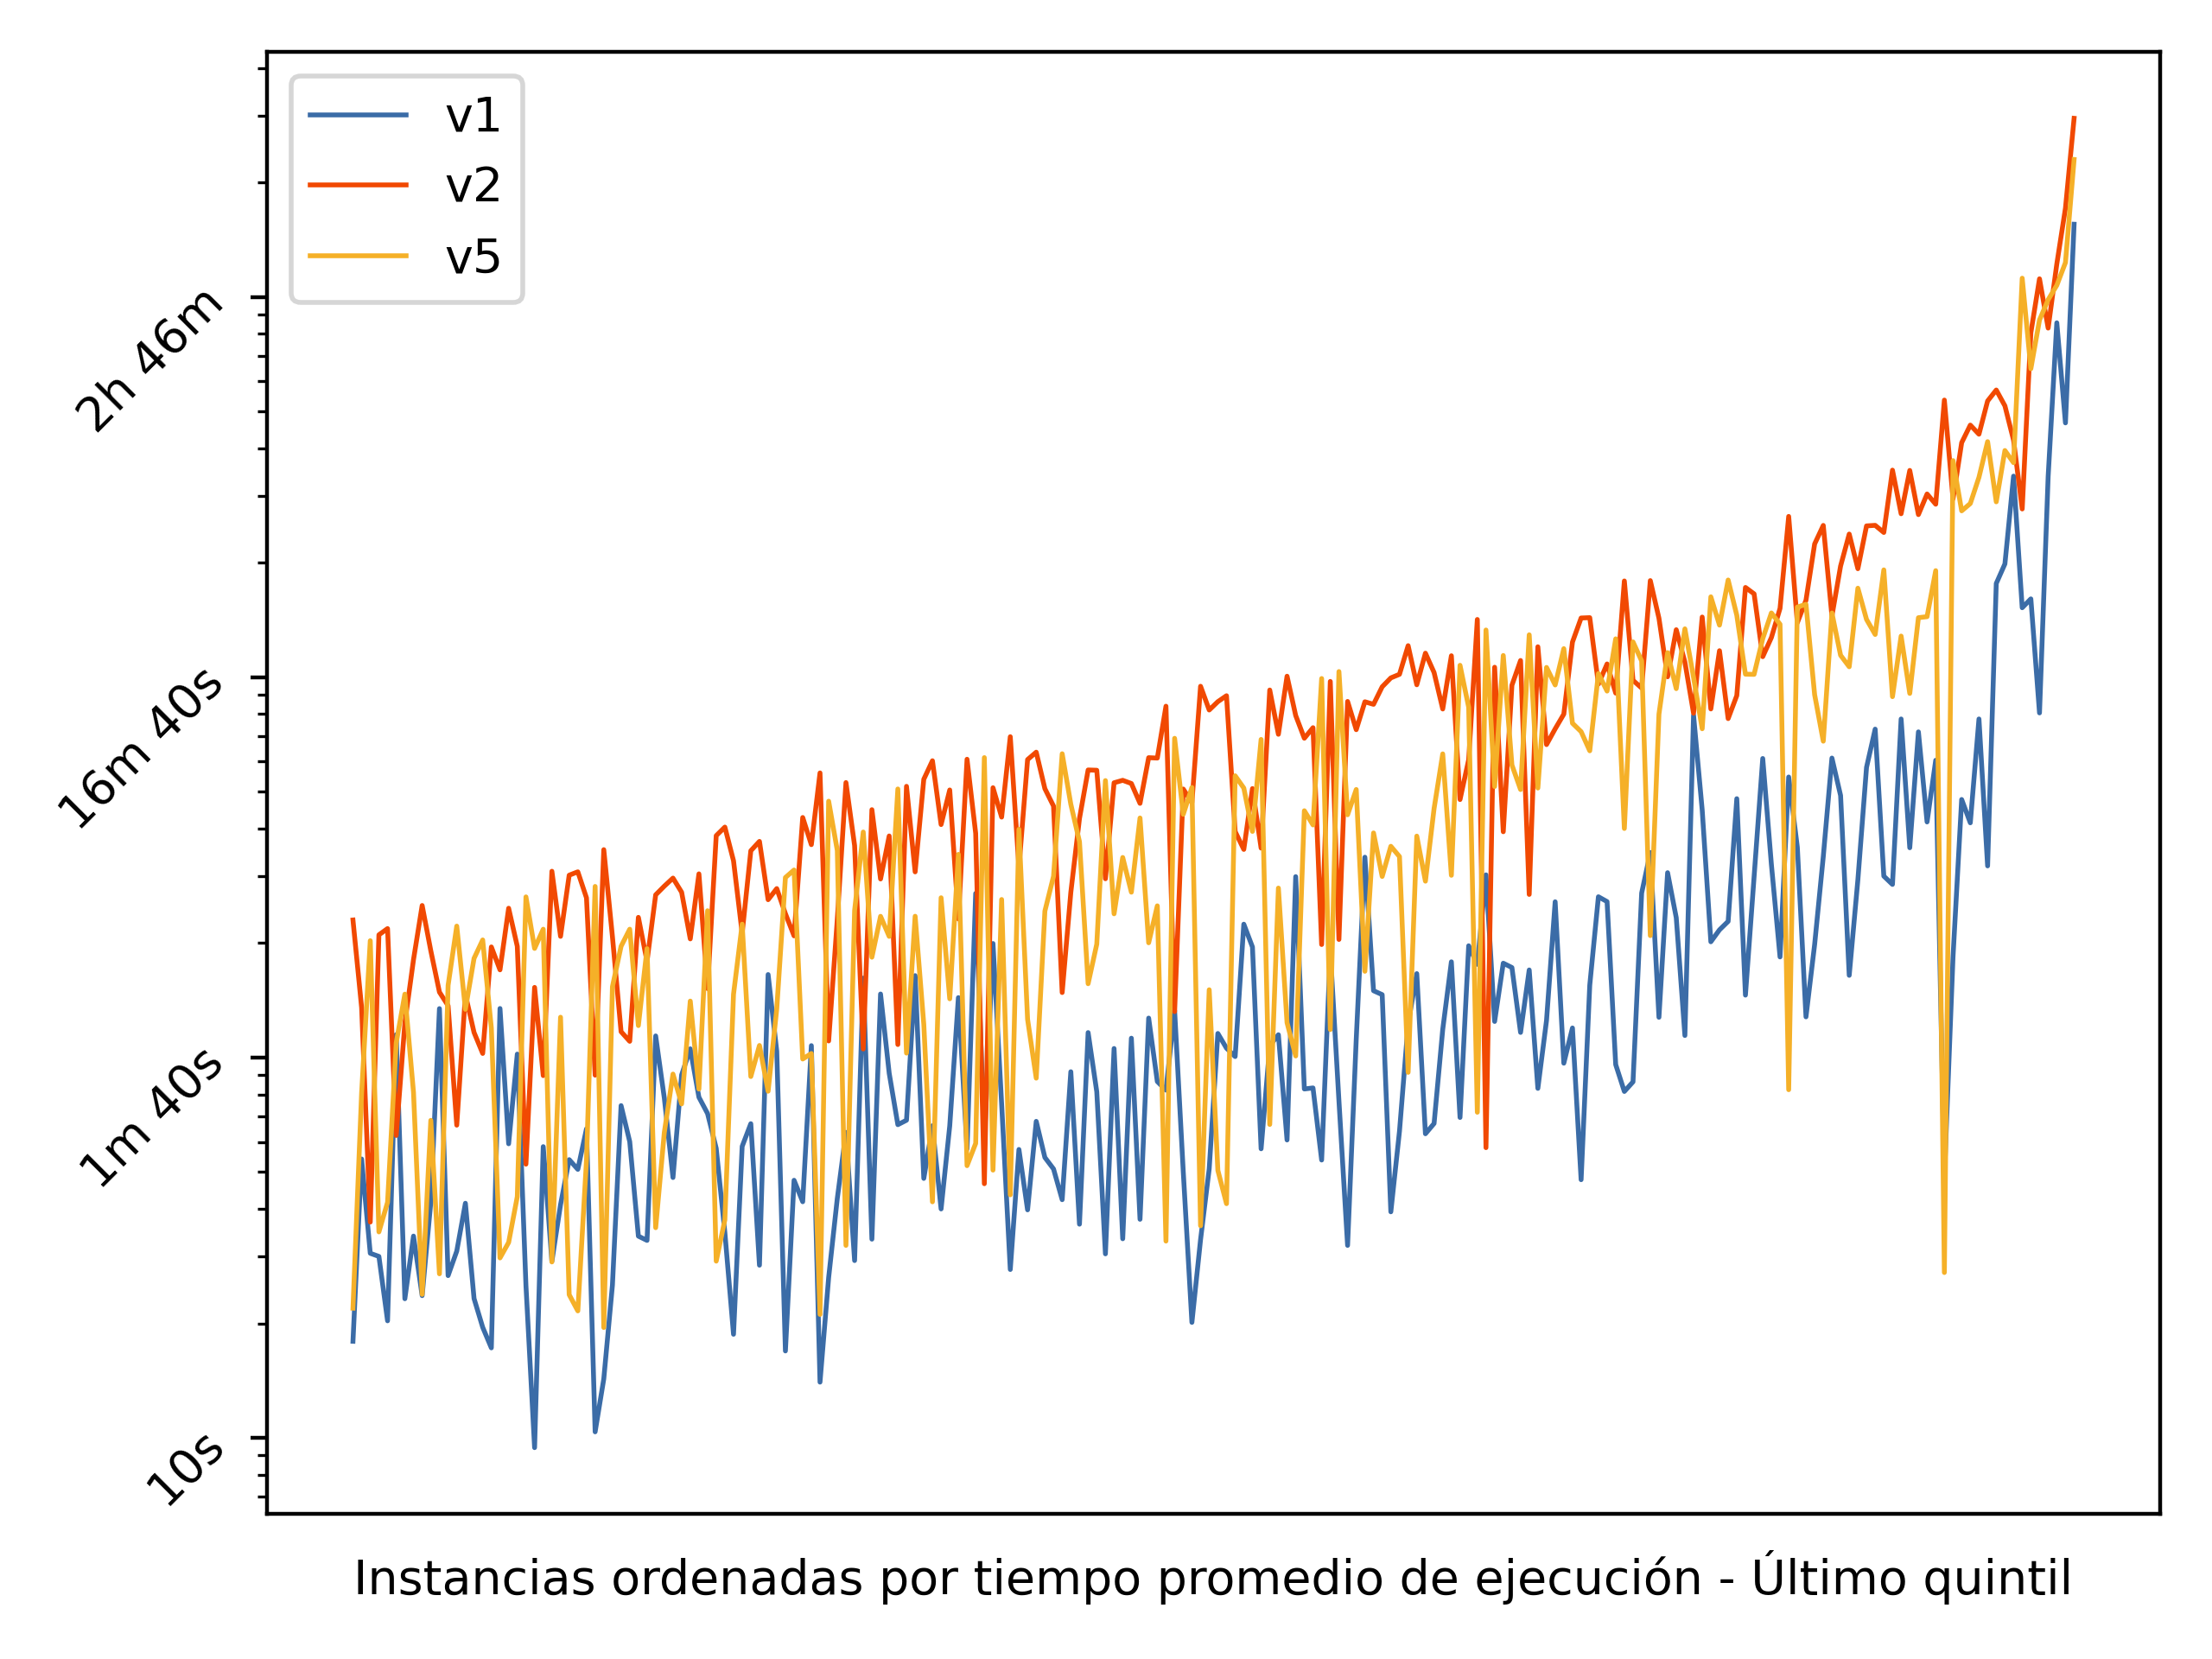
\includegraphics[width=10cm]{../resources/run_time_comparsion_rerun.png}
    \caption{Comparativa del tiempo de ejecución sobre la segunda ronda de instancias en los tres mejores modelos de la primera. La escala es logarítmica en el eje de las ordenadas.} \label{fig:runtimecomparisonrerun}
  \end{figure}

  \begin{figure}[h!]
    \centering
    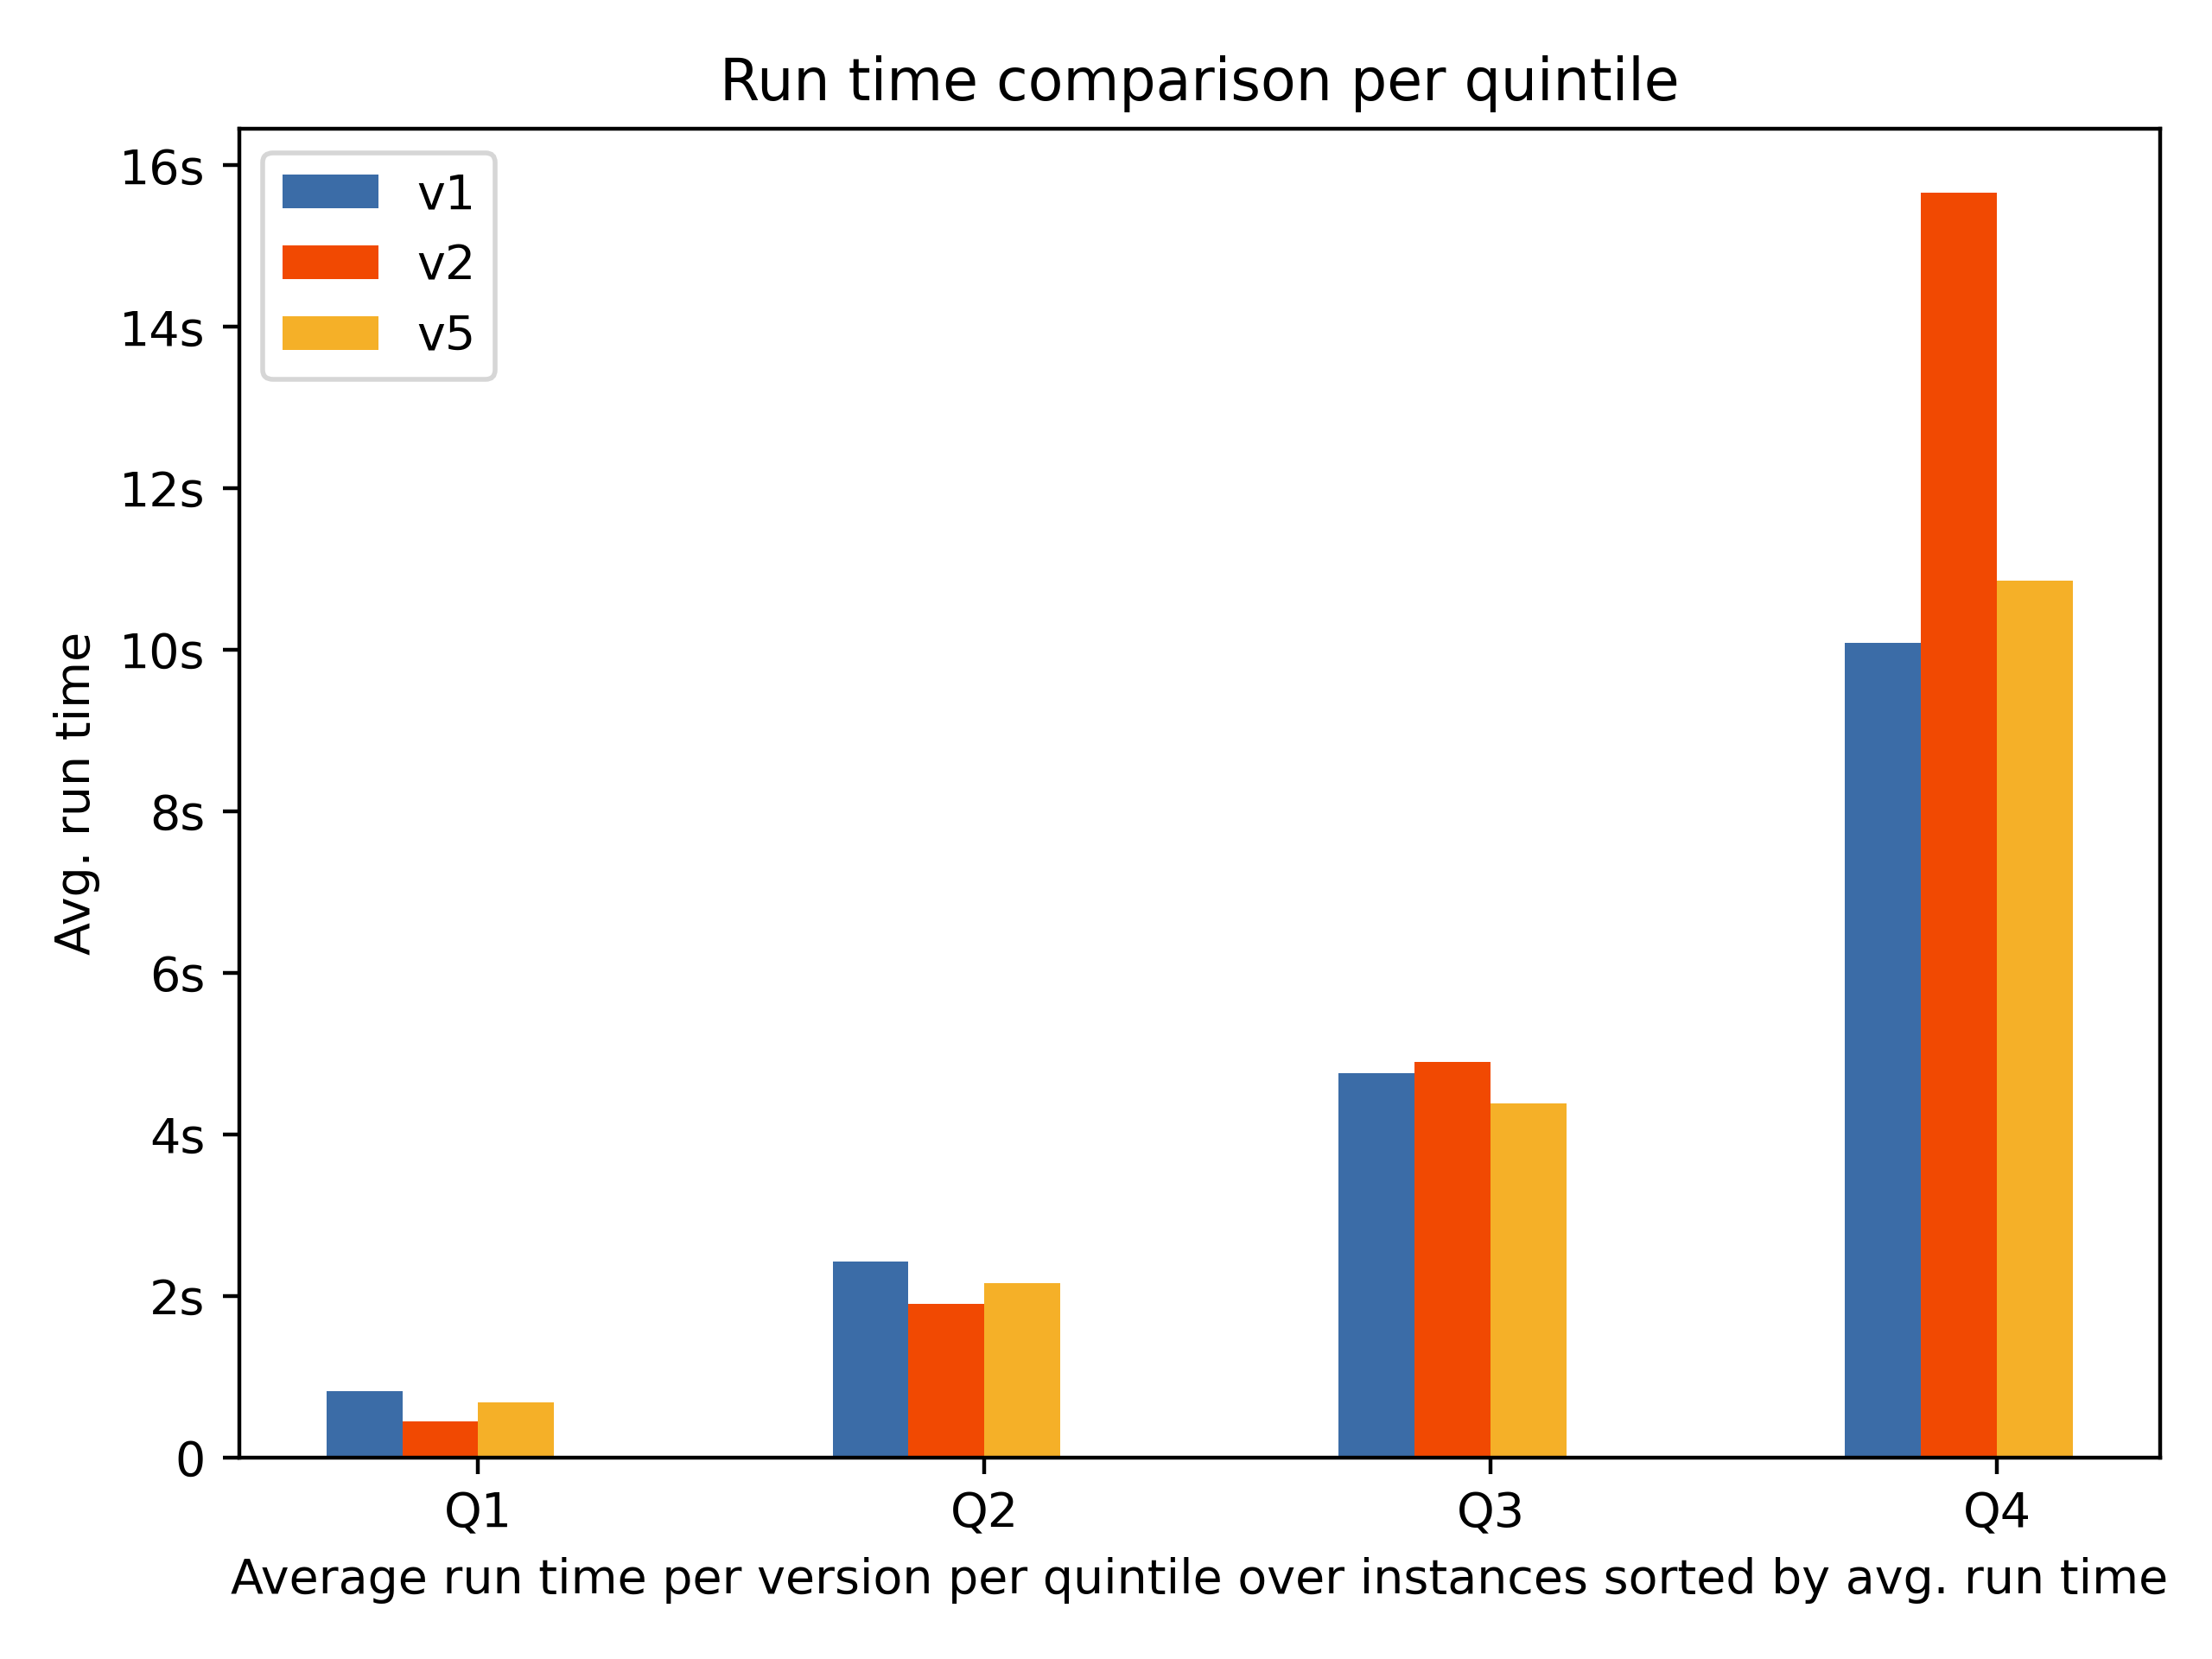
\includegraphics[width=10cm]{../resources/run_time_comparsion_by_quintile_rerun.png}
    \caption{Comparativa del tiempo de ejecución sobre la segunda ronda de instancias en los cuatro primeros quintiles. Las instancias fueron ordenadas por tiempo promedio de ejecución.} \label{fig:firstfourquintilesrerun}
  \end{figure}

  Los resultados de las nuevas ejecuciones se encuentran en la tabla (\ref{table:resumenreejecuciones}) y las figuras (\ref{fig:runtimecomparisonrerun}) y (\ref{fig:firstfourquintilesrerun}). Observamos que se mantiene el comportamiento de la ronda anterior y el v1 sigue siendo más rápido. También observamos que el desempeño de v5 se degradó de peor manera. En los nuevos resultados no hubieron diferencias en términos de demanda total transferida y verificamos correctamente que la diferencia en la instancia problemática de la primera ronda fue solucionada. Dados los resultados, decidimos continuar el resto de este trabajo con la versión v1 de la formulación.

  \section{Resultados computacionales}

  \subsection{Análisis de sensibilidad}

  Estudiamos el comportamiento del modelo frente a perturbaciones en alguno de sus parámetros. Utilizamos la red de Sioux-Falls nuevamente dado que es de un tamaño manejable para realizar todas las ejecuciones en tiempo razonable. Las perturbaciones las realizamos sobre los parámetros específicos del problema, dejando los datos de la red y matriz de demanda fijos. Estos son: puntos de quiebre, funciones de transferencia de demanda y presupuesto. Observar que los parámetros estudiados son de distinta naturaleza: mientras que los primeros dos son relativos al comportamiento de la demanda el último es una decisión exclusiva de la entidad planificadora. La matriz de demanda se toma de Liu 2019 \cite{liu2019}, con 22 pares origen-destino. Los datos de la red y matriz de demanda se encuentran en un apéndice.

  \subsubsection{Especificación de datos}

  Nuestro problema requiere la disponibilidad de parámetros que en la práctica no son fácilmente especificables en términos de un valor escalar. En esta sección definimos algunos criterios que utilizamos para especificarlos en base a trabajos externos. En la siguiente, analizamos qué efectos tienen las perturbaciones sobre las soluciones.

  La cantidad y tipos de infraestructuras de ciclovía varían de país a país tanto en su disponibilidad como en sus costos y por lo tanto es difícil estimar estos últimos de manera general sin llegar a un análisis caso a caso. Por ejemplo en la ciudad de Montevideo podemos encontrar tres tipos \footnote{Mapa interactivo: \url{https://montevideo.gub.uy/mapa-montevideo-en-bici}}: el más básico consiste en imponer un límite bajo de velocidad para los vehículos automotores (30 km/h) y cartelería resaltando cierta calle o zona cómo disponible para el tránsito en bicicleta. Un segundo tipo consiste en utilizar una fracción de la calle como senda específica para bicicletas que puede ir en uno o ambos sentidos. Y el tercer tipo consta de una bicisenda construida especificamente para bicicletas generalmente en canteros y parques.

  Los costos de construcción pueden variar según la ubicación y tipo de ciclovía, congestión del área de la ciudad, precios de insumos externos como el petróleo y cuestiones logísticos como reubicación de paradas de ómnibus y señales de tránsito, entre otros aspectos. Se puede encontrar información al respecto en el análisis {\it Typical Costs of Cycling Interventions} \cite{typicalcostsofcylcing} que presenta diversos tipos de infraestructuras y los principales factores que afectan el costo de construcción como trabajo dentro de un programa de incentivo del transporte en bicicleta en Inglaterra. En este trabajo nos basamos para simplificar y generalizar la estimación de costos en base al tipo de infraestructura: decimos que la infraestructura de tipo $i+1$ cuesta el doble que la infraestructura de tipo $i$.

  Por otro lado, los costos de usuario de atravesar un arco varían en la práctica dependiendo de factores como ancho de la vía, pavimento, volumen y velocidad del tránsito, entre otros, que a su vez se ponderan por el largo del arco. En el documento {\it Bicycle Level Of Service, Applied Model} \cite{blos2007} podemos encontrar el concepto de {\it Bicycle Level of Service} (BLOS), muy utilizado en la literatura, que agrupa estas consideraciones bajo un único valor. Para el cálculo del BLOS se tienen en cuenta los distintos aspectos que cuantificados en indicadores, son luego utilizados en una fórmula para calcular el puntaje de BLOS que se estratifican según el documento en 6 niveles del A al F.

  Los aspectos que se consideran son los siguientes:

  \begin{enumerate}
    \item{Ancho promedio de la banquina, presencia de ciclovía, porcentaje de la vía ocupada por estacionamiento}
    \item{Límite de velocidad de vehículos motorizados}
    \item{Volumen promedio de los vehículos motorizados}
    \item{Porcentaje de tránsito pesado (camiones)}
    \item{Condición del pavimento}
  \end{enumerate}

  \begin{table}[h!]
    \centering
    \caption*{{\bf Niveles de BLOS}}
    \begin{tabular}{cccc}
      \toprule
        Nivel & Puntaje BLOS & Infraestructura & \shortstack{Proporción de mejora \\ sobre costo base} \\
      \midrule
        A     & $\leq 1.5$   & 5              & 0.4   \\
        B     & 1.5-2.5      & 4              & 0.52  \\
        C     & 2.5-3.5      & 3              & 0.64  \\
        D     & 3.5-4.5      & 2              & 0.76  \\
        E     & 4.5-5.5      & 1              & 0.88  \\
        F     & > 5.5        & 0              & 1     \\
      \bottomrule
    \end{tabular}
    \caption{Niveles de servicio definidos en el BLOS, menor puntaje BLOS representa mejores condiciones para el usuario. Para cada nivel se define una infraestructura y su correspondiente proporción de mejora sobre la infraestructura base.}\label{table:blosscores}
  \end{table}

  Tomando como base el puntaje de BLOS estratificado de la tabla (\ref{table:blosscores}), podemos traducir de forma aproximada los puntajes de BLOS a proporción de mejora sobre la infraestructura base o red de calles utilizando la función $C_{infra}(i) = {28 - 3 (i + 1) \over 25}$ donde $i \in I = \{0,1,2,\ldots\}$ es el tipo de infraestructura. Suponiendo que el nivel F de la escala de BLOS corresponde a infraestructura base (o infraestructura 0), la proporción de mejora de las infraestructuras A-E correspondientes a los tipos de infraestructura 5,4,3,2 y 1 respectivamente se pueden observar en la misma tabla.

  Incurrimos a la simplificación de considerar, al definir una instancia, la cantidad $T$ de tipos infraestructuras posibles a utilizar y no cuáles, de manera que las infraestructuras utilizables sean $I = \{0,.., T - 1\}$. Dada una instancia del problema, llamamos $m$ a la proporción de mejora máxima que puede dar la mejor infraestructura de entre las disponibles, es decir $m = C_{infra}(T - 1)$. El valor $m$ es de utilidad al definir las funciones de transferencia de demanda como veremos a continuación.

  Respecto al comportamiento de los usuarios, suponemos que la demanda de todos los pares origen-destino se comporta de igual manera, lo cual tiene sentido al considerar una población determinada. Esto reduce la necesidad de especificar $|OD|$ funciones de transferencias de demanda a una sola. Es decir, para cada par origen destino $k$, tenemos que $f_k(w_k) = f({w_k \over S^{best}_k})D_k$, donde $D_k$ es la demanda máxima que se puede transferir, $S^{best}_k$ es el costo del camino más corto sobre la infraestructura base y $f: [m, 1] \rightarrow [0, 1]$ modela la proporción de demanda transferida en función de la proporción del nuevo costo sobre el costo base $S^{best}_k$.

  Partimos del trabajo {\it Performance evaluation of extreme bicycle scenarios} \cite{shwe2014} que analizando una extensiva encuesta realizada en varios países aproxima la proporción de viajes hechos en bicicleta y el largo de infraestructura de ciclovía per cápita en la ciudad a una relación lineal. Tomando este resultado, utilizamos una función lineal decreciente como función de transferencia de referencia. Como alternativa, encontramos en el libro {\it Modeling Transport} \cite{ortuz2011} que el comportamiento de la demanda al momento de decidir entre dos modos se comporta como una función con forma de S, logística o sigmoide, por lo que también consideramos una función logística en nuestras pruebas. Por completitud analizamos otras funciones que podrían considerarse razonables: una con concavidad estrictamente positiva y otra con concavidad estrictamente negativa en el intervalo $[m, 1]$.

  Establecer valores de presupuesto realistas depende altamente de las condiciones políticas y económicas de cada localidad. Podemos encontrar en la literatura \cite{rios2015} y \cite{shwe2014} que factores de cubrimiento de la red de ciclovías en una ciudad de entre 10\% y 40\% del total de la superficie de una ciudad están dentro de los parámetros normales. Seguimos este enfoque y especificamos el presupuesto como porcentaje del costo total de construir una infraestructura en toda la red tomando como referencia el costo de la infraestructura 1, es decir la infraestructura especializada más básica. Dado nuestro método para el calculo de los costos de los tipos de infraestructuras esto implica que un presupuesto del 40\% es suficientemente para cubrir 20\% solo con la infraestructura de tipo 2, 10\% solo con la infraestructura de tipo 3; y en general un factor de $F\%$ cubre ${F \over {2^{i - 1}}}\%$ de la infraestructura $i \in \{1,..,5\}$.

  Finalmente, usamos el largo de los arcos como costo de usuario y costo de construcción de la infraestructura 1. Esto nos da una medida suficientemente simple y general como para usar en cualquier instancia.

  \FloatBarrier
  \subsubsection{Perturbaciones}

  Uno de nuestros objetivos es determinar cuáles son las perturbaciones, mas allá de un incremento en el presupuesto, que resultan en mayores valores de demanda transferida total. Por un lado, la cantidad de infraestructuras disponibles es determinante respecto a la mejora alcanzable en los caminos. Es de esperar que el modelo decida utilizar mejores infraestructuras en los arcos con mayor flujo de demanda, tanto como el presupuesto y tipos de infraestructuras disponibles lo permitan. En principio no hay razón para limitar este número a un valor distinto del mayor valor posible, a menos que el deterioro en el tiempo de ejecución lo haga necesario. Respecto a los puntos de quiebre esperamos que una mayor granularidad aporte positivamente a nuestro objetivo, aunque, al igual que la cantidad de infraestructuras, tendremos cuidado con deterioro en el desempeño.

  Como instancia de referencia consideramos la red de Sioux-Falls y matriz de demanda antedicha y el siguiente conjunto de parámetros en base a la discusión de la sección anterior:

  \begin{description}
    \item[Infraestructuras]: 5 infraestructuras además de la base.
    \item[Puntos de quiebre]: Función lineal de transferencia de demanda con 5 puntos de quiebre.
    \item[Presupuesto]: Factor de presupuesto del 80\%.
  \end{description}

  Las perturbaciones las realizamos sobre el conjunto de parámetros de la instancia de referencia aplicando una o dos perturbaciones por vez en lugar de ejecutar todas las posibles combinaciones de parámetros perturbados, ya que esto implicaría una mayor cantidad de instancias a estudiar.

  En primer lugar analizamos la sensibilidad respecto al factor de presupuesto. Los valores utilizados son: 10\%, 80\%, 160\% y 320\%. El objetivo es observar si se cumple la simple intuición de que siempre a mayor presupuesto se obtienen mejores resultados y cómo es el comportamiento respecto a los incrementos de presupuesto. También analizamos el efecto que tiene la cantidad de puntos de quiebre en los resultados, utilizando 5 y 20 puntos para cada presupuesto.

  Luego, comparamos el resultado de aplicar diferentes funciones de transferencia de demanda y cómo afecta el hecho de utilizar distintas cantidades de puntos de quiebre. Utilizamos 5, 20 y 50 puntos de quiebre junto a las cuatro funciones mencionadas en la sección anterior. Los puntos los definimos de manera que sean equidistantes en el codominio, es decir, si hay N puntos, de un punto al siguiente se obtiene una mejora de aproximadamente ${1 \over N - 1}$ en la proporción de demanda transferida.

  Como resultado tenemos 36 instancias cuya representación pre simplificaciones en Simplex son matrices que van desde un tamaño de 12597x12310 con 562 variables enteras hasta 14487x14290 con 1552 variables enteras.

  \begin{figure}[h!]
    \centering
    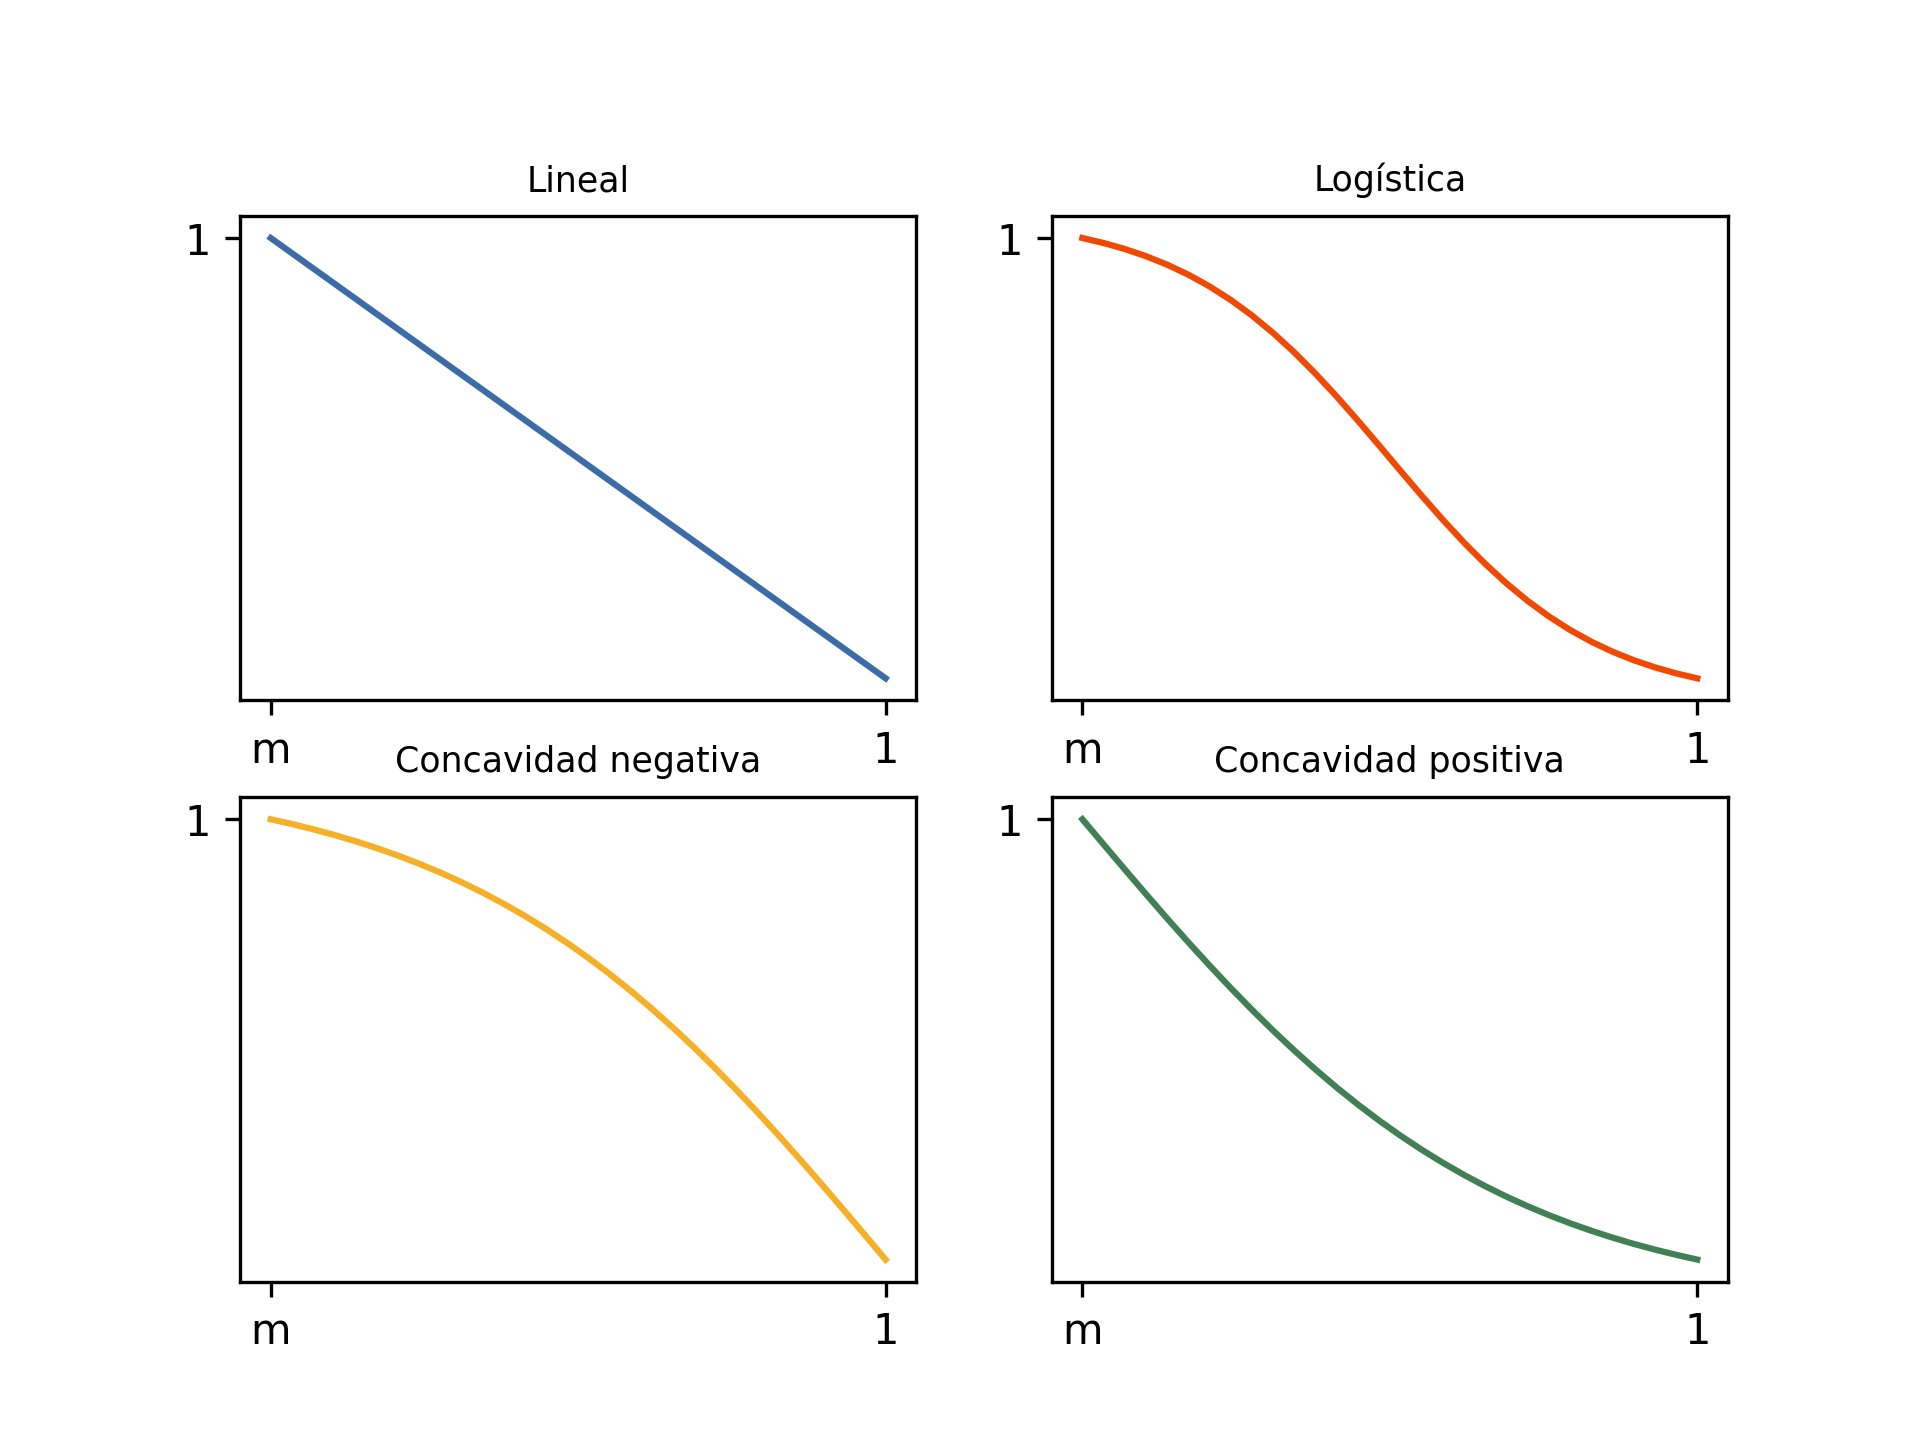
\includegraphics[width=8cm]{../resources/f_catalog.png}
      \caption{Catálogo de funciones usadas para modelar la transferencia de demanda a la bicicleta. El valor de $m$ varía según las infraestructuras utilizadas y equivale a la proporción mínima alcanzada por la mejor infraestructura utilizada, es decir $m = min_{i \in I} \{ C_{infra}(i) \}$.}
    \label{fig:fcatalog}
  \end{figure}

  \FloatBarrier
  \subsubsection{Resultados}

  Las instancias fueron ejecutadas con el solver CPLEX versión 12.8.0.0 en su configuración por defecto sobre una maquina Intel Core i9-9900K con 64GiB de RAM. Los resultados generales de las ejecuciones se encuentran en la tabla (\ref{table:sensibilityresults}) y los datos sobre el uso del presupuesto, que luego comentaremos, en la tabla (\ref{table:sensibilitybudgetusage}).

  Se puede observar que a mayor cantidad de puntos de quiebre, fijando la función de transferencia de demanda y el presupuesto, obtenemos mayor transferencia de demanda. Esto tiene sentido ya que la función de transferencia es representada de manera más precisa. También vemos que variar la cantidad de puntos de quiebre parece hacer variar enormemente el tiempo de ejecución en algunos casos, sin poderse determinar una relación directa entre la cantidad y la complejidad resultante, aunque entendemos que para sacar conclusiones al respecto deberíamos realizar un buen número de ejecuciones para cada instancia en lo que en CPLEX se llama modo oportunista, es decir paralelizar al máximo sin garantizar determinismo. Por otro lado, observamos un fuerte impacto del modelado del comportamiento de la transferencia de demanda, es decir de cuál función se utiliza, sobre la demanda transferida. Esto nos confirma que es un aspecto importante del modelado, si bien las funciones consideradas en este caso pueden haber sido irreales o exageradas en sus curvaturas. Finalmente, vemos que la demanda transferida en función de la cantidad de presupuesto, fijando cantidad de puntos de quiebre y función de transferencia de demanda, parece crecer según la curva de la figura (\ref{fig:demandtransferbybudgetlinear}) con concavidad negativa lo que implica que el beneficio marginal de aumentar el presupuesto es cada vez menor.

  \begin{figure}[h!]
    \centering
    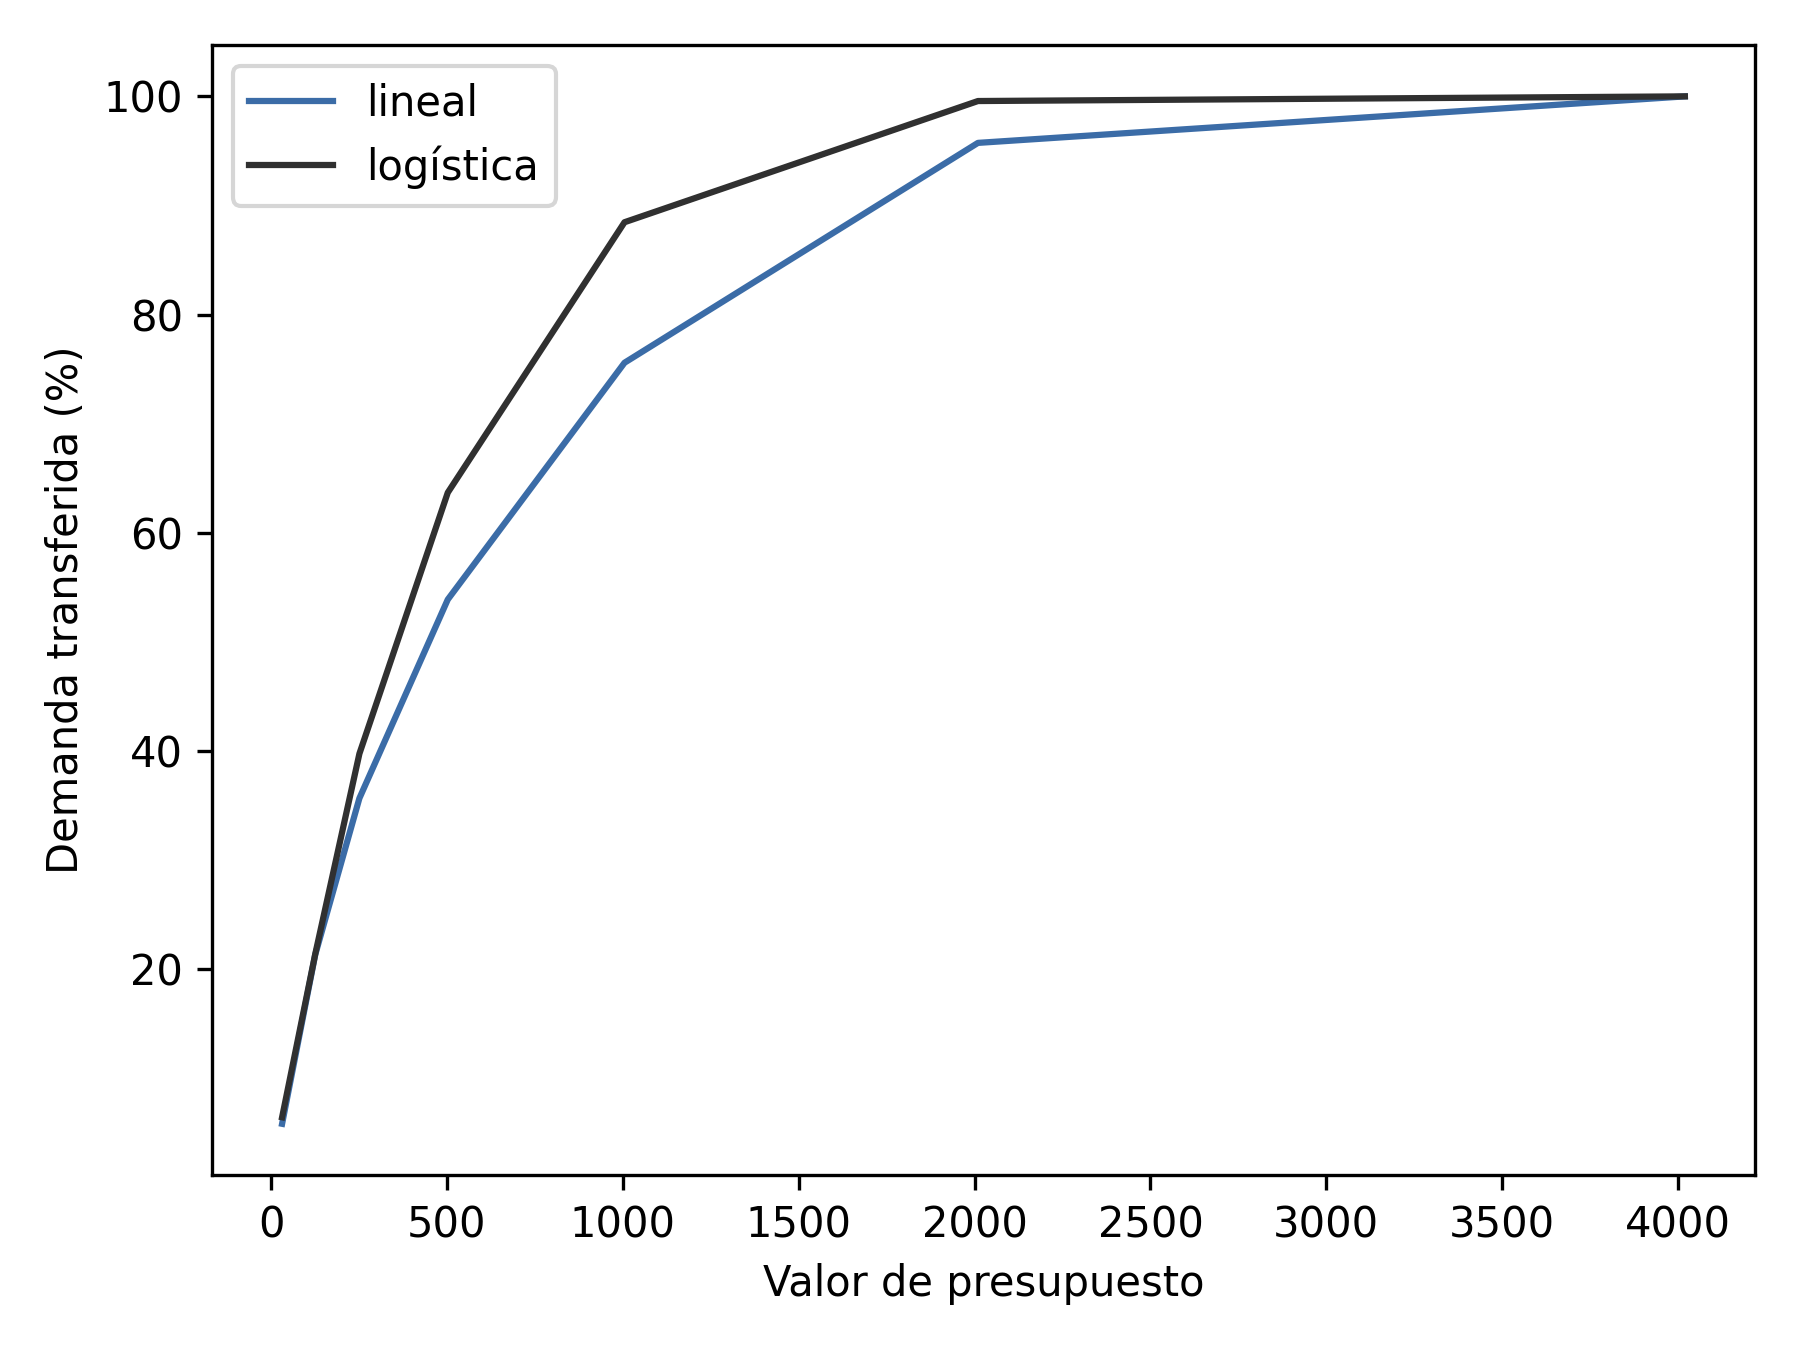
\includegraphics[width=8cm]{../resources/demand_by_budget.png}
      \caption{Porcentaje de demanda transferida total en función del presupuesto asignado para Sioux-Falls utilizando 20 puntos de quiebre y las funciones de transferencia de demanda lineal y logit. El comportamiento es similar en ambos casos y muestra que la eficiencia de aumentar el presupuesto no es siempre la misma.}
    \label{fig:demandtransferbybudgetlinear}
  \end{figure}

  Respecto a la utilización del presupuesto, vemos que a mayor presupuesto mayor es el porcentaje de gasto en los tipos de infraestructuras más caras, lo cual es esperable dado que benefician mas al usuario. Por otro lado, aumentar la cantidad de puntos de quiebre manteniendo presupuesto y función de transferencia fijas hace que el gasto en los tipos de infraestructuras varíe, no necesariamente concentrando el gasto en los tipos más caros. El desglose del presupuesto utilizado por infraestructura se detalla en la tabla (\ref{table:sensibilitybudgetusage}) y en la figura (\ref{fig:sensibilitybudgetusage}).

  \begin{sidewaystable}
    \centering
    \caption*{{\bf Ejecuciones del análisis de sensibilidad de parámetros}}
    \begin{tabular}{cccccc}
        \toprule
        Instancia & Factor de presupuesto & \shortstack{Cantidad de puntos \\ de quiebre} & Función $f$ & Demanda transferida (\%) & \shortstack{Tiempo ejecución \\ (HH:MM:SS)} \\
        \midrule
        1 & 0,1 & 5 & lineal & 4,65 & 00:00:02 \\
        2 & 0,1 & 20 & lineal & 5,81 & 00:00:11 \\
        3 & 0,1 & 5 & logit & 5,13 & 00:00:01 \\
        4 & 0,1 & 20 & logit & 6,41 & 00:00:08 \\
        5 & 0,4 & 5 & concave down & 32,43 & 00:00:36 \\
        6 & 0,4 & 20 & concave down & 36,49 & 00:07:40 \\
        7 & 0,4 & 50 & concave down & 37,39 & 00:07:29 \\
        8 & 0,4 & 5 & concave up & 15,50 & 00:00:18 \\
        9 & 0,4 & 20 & concave up & 17,05 & 00:09:38 \\
        10 & 0,4 & 50 & concave up & 18,22 & 14:07:09 \\
        11 & 0,4 & 5 & lineal & 18,60 & 00:00:24 \\
        12 & 0,4 & 20 & lineal & 21,32 & 00:06:17 \\
        13 & 0,4 & 50 & lineal & 22,09 & 00:31:55 \\
        14 & 0,4 & 5 & logit & 18,80 & 00:00:27 \\
        15 & 0,4 & 20 & logit & 21,37 & 00:12:35 \\
        16 & 0,4 & 50 & logit & 23,08 & 00:43:53 \\
        17 & 0,8 & 5 & lineal & 32,17 & 00:00:59 \\
        18 & 0,8 & 20 & lineal & 35,66 & 01:26:32 \\
        19 & 0,8 & 5 & logit & 35,47 & 00:00:44 \\
        20 & 0,8 & 20 & logit & 39,74 & 00:05:20 \\
        21 & 1,6 & 5 & lineal & 49,22 & 00:03:22 \\
        22 & 1,6 & 20 & lineal & 53,88 & 00:55:20 \\
        23 & 1,6 & 5 & logit & 58,97 & 00:02:36 \\
        24 & 1,6 & 20 & logit & 63,68 & 00:35:05 \\
        25 & 3,2 & 5 & lineal & 71,71 & 00:00:54 \\
        26 & 3,2 & 20 & lineal & 75,58 & 00:07:49 \\
        27 & 3,2 & 5 & logit & 80,77 & 00:01:33 \\
        28 & 3,2 & 20 & logit & 88,46 & 00:02:39 \\
        29 & 6,4 & 5 & lineal & 94,57 & 00:00:05 \\
        30 & 6,4 & 20 & lineal & 95,74 & 00:00:22 \\
        31 & 6,4 & 5 & logit & 97,44 & 00:00:02 \\
        32 & 6,4 & 20 & logit & 99,57 & 00:00:01 \\
        33 & 12,8 & 5 & lineal & 100,00 & 00:00:00 \\
        34 & 12,8 & 20 & lineal & 100,00 & 00:00:00 \\
        35 & 12,8 & 5 & logit & 100,00 & 00:00:00 \\
        36 & 12,8 & 20 & logit & 100,00 & 00:00:00 \\
        \bottomrule
    \end{tabular}
      \caption{Todas las instancias fueron solucionadas al óptimo en tiempos relativamente cortos, con excepción de dos instancias cuyo tiempo de ejecución fue más de una hora.} \label{table:sensibilityresults}
  \end{sidewaystable}

  \begin{sidewaystable}
    \centering
    \caption*{{\bf Presupuesto utilizado por tipo de infraestructura}}
    \begin{tabular}{cccccccc}
        \toprule
        Instancia & Presupuesto & Presupuesto utilizado & Infra. 1 (\%) & Infra. 2 (\%) & Infra. 3 (\%) & Infra. 4 (\%) & Infra. 5 (\%) \\
        \midrule
        1 & 31,4 & 31 & 35,03 & 63,69 &  &  &  \\
        2 & 31,4 & 31 & 9,55 & 89,17 &  &  &  \\
        3 & 31,4 & 30 &  & 44,59 & 50,96 &  &  \\
        4 & 31,4 & 31 & 9,55 & 50,96 & 38,22 &  &  \\
        5 & 125,6 & 125 & 10,35 & 82,80 & 6,37 &  &  \\
        6 & 125,6 & 125 & 3,98 & 89,17 & 6,37 &  &  \\
        7 & 125,6 & 125 & 5,57 & 81,21 & 12,74 &  &  \\
        8 & 125,6 & 125 & 2,39 & 23,89 & 41,40 & 31,85 &  \\
        9 & 125,6 & 125 & 7,17 & 12,74 & 47,77 & 31,85 &  \\
        10 & 125,6 & 125 & 2,39 & 27,07 & 50,96 & 19,11 &  \\
        11 & 125,6 & 125 & 15,13 & 33,44 & 50,96 &  &  \\
        12 & 125,6 & 125 & 16,72 & 70,06 & 12,74 &  &  \\
        13 & 125,6 & 125 & 5,57 & 81,21 & 12,74 &  &  \\
        14 & 125,6 & 125 & 3,98 & 44,59 & 38,22 & 12,74 &  \\
        15 & 125,6 & 125 & 5,57 & 11,15 & 70,06 & 12,74 &  \\
        16 & 125,6 & 125 & 2,39 & 36,62 & 60,51 &  &  \\
        17 & 251,2 & 251 & 5,18 & 35,83 & 36,62 & 22,29 &  \\
        18 & 251,2 & 251 & 8,36 & 21,50 & 70,06 &  &  \\
        19 & 251,2 & 251 & 1,99 & 21,50 & 44,59 & 31,85 &  \\
        20 & 251,2 & 251 & 1,19 & 11,15 & 81,21 & 6,37 &  \\
        21 & 502,4 & 502 & 0,40 & 15,92 & 19,90 & 63,69 &  \\
        22 & 502,4 & 502 & 2,39 & 7,56 & 45,38 & 44,59 &  \\
        23 & 502,4 & 501 & 2,19 & 13,93 & 35,83 & 47,77 &  \\
        24 & 502,4 & 502 & 2,79 & 5,57 & 54,94 & 36,62 &  \\
        25 & 1004,8 & 1002 & 0,40 & 4,18 & 13,14 & 19,90 & 62,10 \\
        26 & 1004,8 & 1004 &  & 5,97 & 6,37 & 49,36 & 38,22 \\
        27 & 1004,8 & 1004 & 0,60 & 2,99 & 26,27 & 17,52 & 52,55 \\
        28 & 1004,8 & 1004 & 0,80 & 1,19 & 14,33 & 83,60 &  \\
        29 & 2009,6 & 2008 &  & 0,40 & 4,38 & 3,58 & 91,56 \\
        30 & 2009,6 & 2008 &  & 0,40 & 1,59 & 10,35 & 87,58 \\
        31 & 2009,6 & 2008 & 0,10 & 1,49 & 2,39 & 1,99 & 93,95 \\
        32 & 2009,6 & 2004 &  & 0,60 & 1,59 & 14,73 & 82,80 \\
        33 & 4019,2 & 2719 & 0,17 & 0,20 & 0,80 &  & 66,48 \\
        34 & 4019,2 & 3048 &  & 0,20 &  &  & 75,64 \\
        35 & 4019,2 & 2780 & 0,10 & 0,60 &  &  & 68,47 \\
        36 & 4019,2 & 2994 & 0,05 &  & 0,40 &  & 74,04 \\
        \bottomrule
    \end{tabular}
      \caption{Detalle de presupuesto utilizado por instancia por tipo de infraestructura. Las columnas Presupuesto y Presupuesto Utilizado están en unidades de presupuesto.} \label{table:sensibilitybudgetusage}
  \end{sidewaystable}

  \begin{figure}[h!]
    \centering
    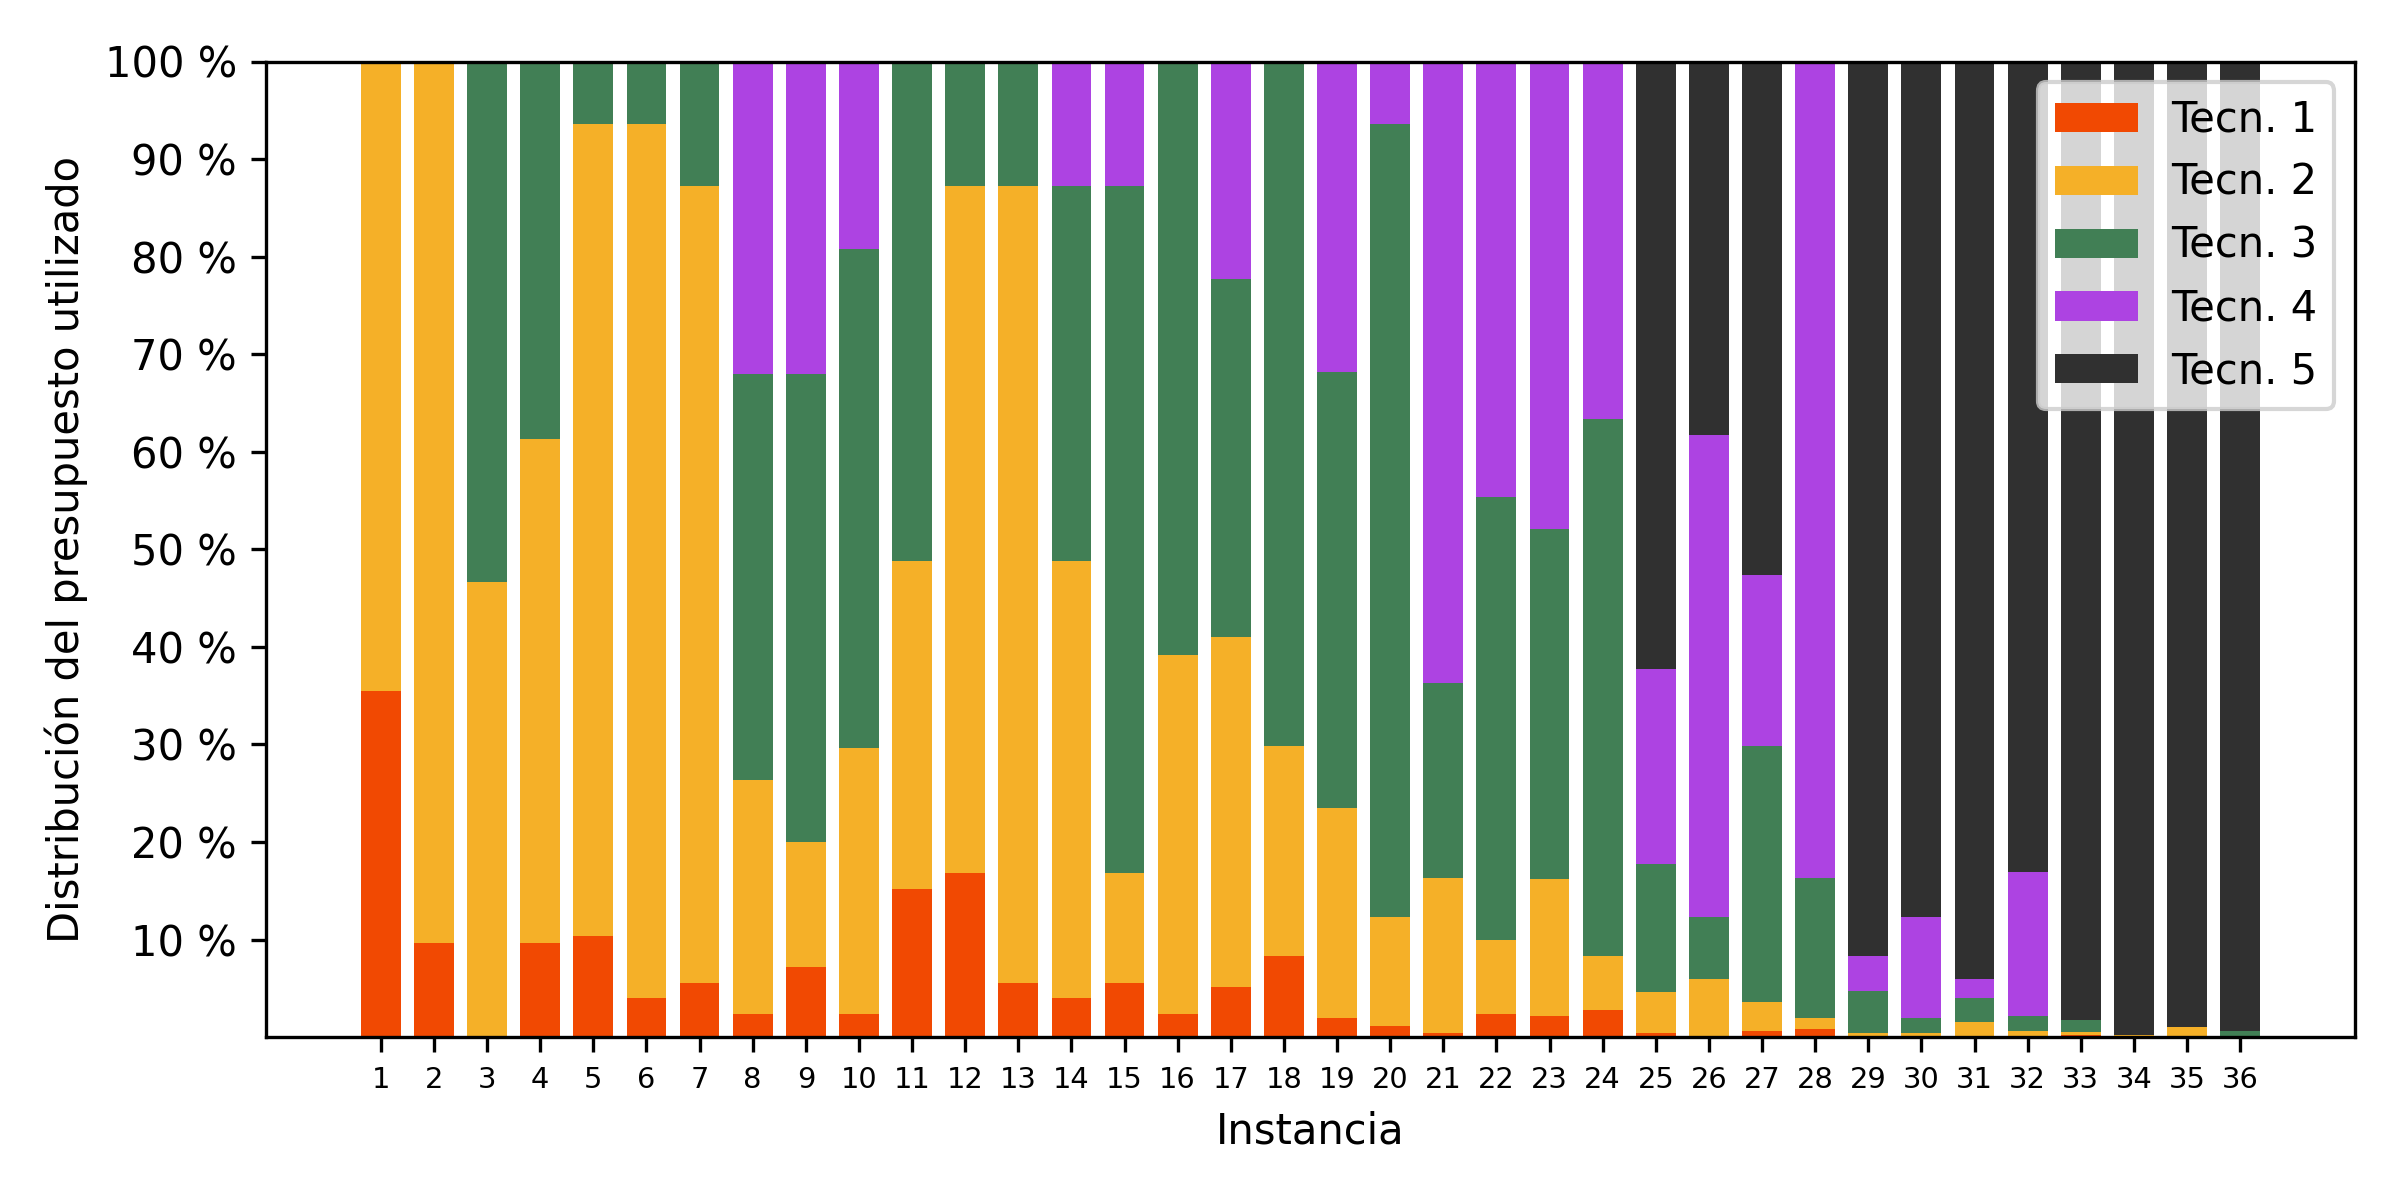
\includegraphics[width=10cm]{../resources/budget_use_by_infra.png}
      \caption{Visualización de la distribución del uso del presupuesto para cada instancia.}
    \label{fig:sensibilitybudgetusage}
  \end{figure}

  \FloatBarrier
  \subsubsection*{Casos interesantes}

  Como caso interesante de comparación vamos a discutir cómo afecta la cantidad de puntos de quiebre a la decisiones de cuales infraestructuras construir. Comparamos las instancias 11, 12 y 13, que utilizan la función lineal de transferencia de demanda con 5, 20 y 50 puntos de quiebre respectivamente y un factor de presupuesto de 40\%. Más datos específicos de cada instancia se pueden apreciar en la tabla (\ref{table:sensibilityinfralengths}) y figura (\ref{fig:sensibilityinstance11_12_13}). Observamos que a mayor cantidad de puntos de quiebre más inteligentes son las decisiones tomadas. Por ejemplo, en la instancia 11 la mitad del acotado presupuesto se invirtió en poco recorrido utilizando la infraestructura 3 mientras que en la 12 y 13 el gasto en esta infraestructura sólo fue el 12\%. En las instancias 12 y 13 la mayor parte del gasto se hizo en infraestructura 2 que para el nivel de presupuesto y función de transferencia de demanda parece ser la más eficiente. En particular, los datos de porcentaje del largo total cubierto desglosado por tipo de infraestructura nos da una idea general de la demanda afectada, al ser esta instancia altamente densa y uniforme en términos de orígenes y destinos, como se observa en la figura (\ref{fig:sioux_falls_demand}).

  Si observamos los datos de demanda transferida y costo de camino más corto, figura (\ref{fig:sensibilitybyodpair_11_12_13}), vemos que a mayor cantidad de puntos de quiebre mayor es la cantidad de pares origen-destino afectada aunque en general las decisiones de cuáles pares origen-destino y cuánto mejorarlos no fue muy diferente entre instancias.

  \begin{table}[h!]
    \centering
    \caption*{{\bf Cobertura de cada tipo de infraestructura}}
    \begin{tabular}{ccccc}
      \toprule
        Instancia & Infra. 1 (\%) & Infra. 2 (\%) & Infra. 3 (\%) & Total (\%) \\
      \midrule
        11 & 8.74  & 6.51   & 5.72 & 20.98 \\
        12 & 8.89  & 15.22  & 1.64 & 25.75 \\
        13 & 2.29  & 17.77  & 1.96 & 22.73 \\
      \bottomrule
    \end{tabular}
    \caption{Porcentaje del largo total de arcos de la red construido con cada tipo de infraestructura (excluyendo la infraestructura base) para las instancias de interés.}\label{table:sensibilityinfralengths}
  \end{table}

  \begin{figure}[h!]
    \centering
    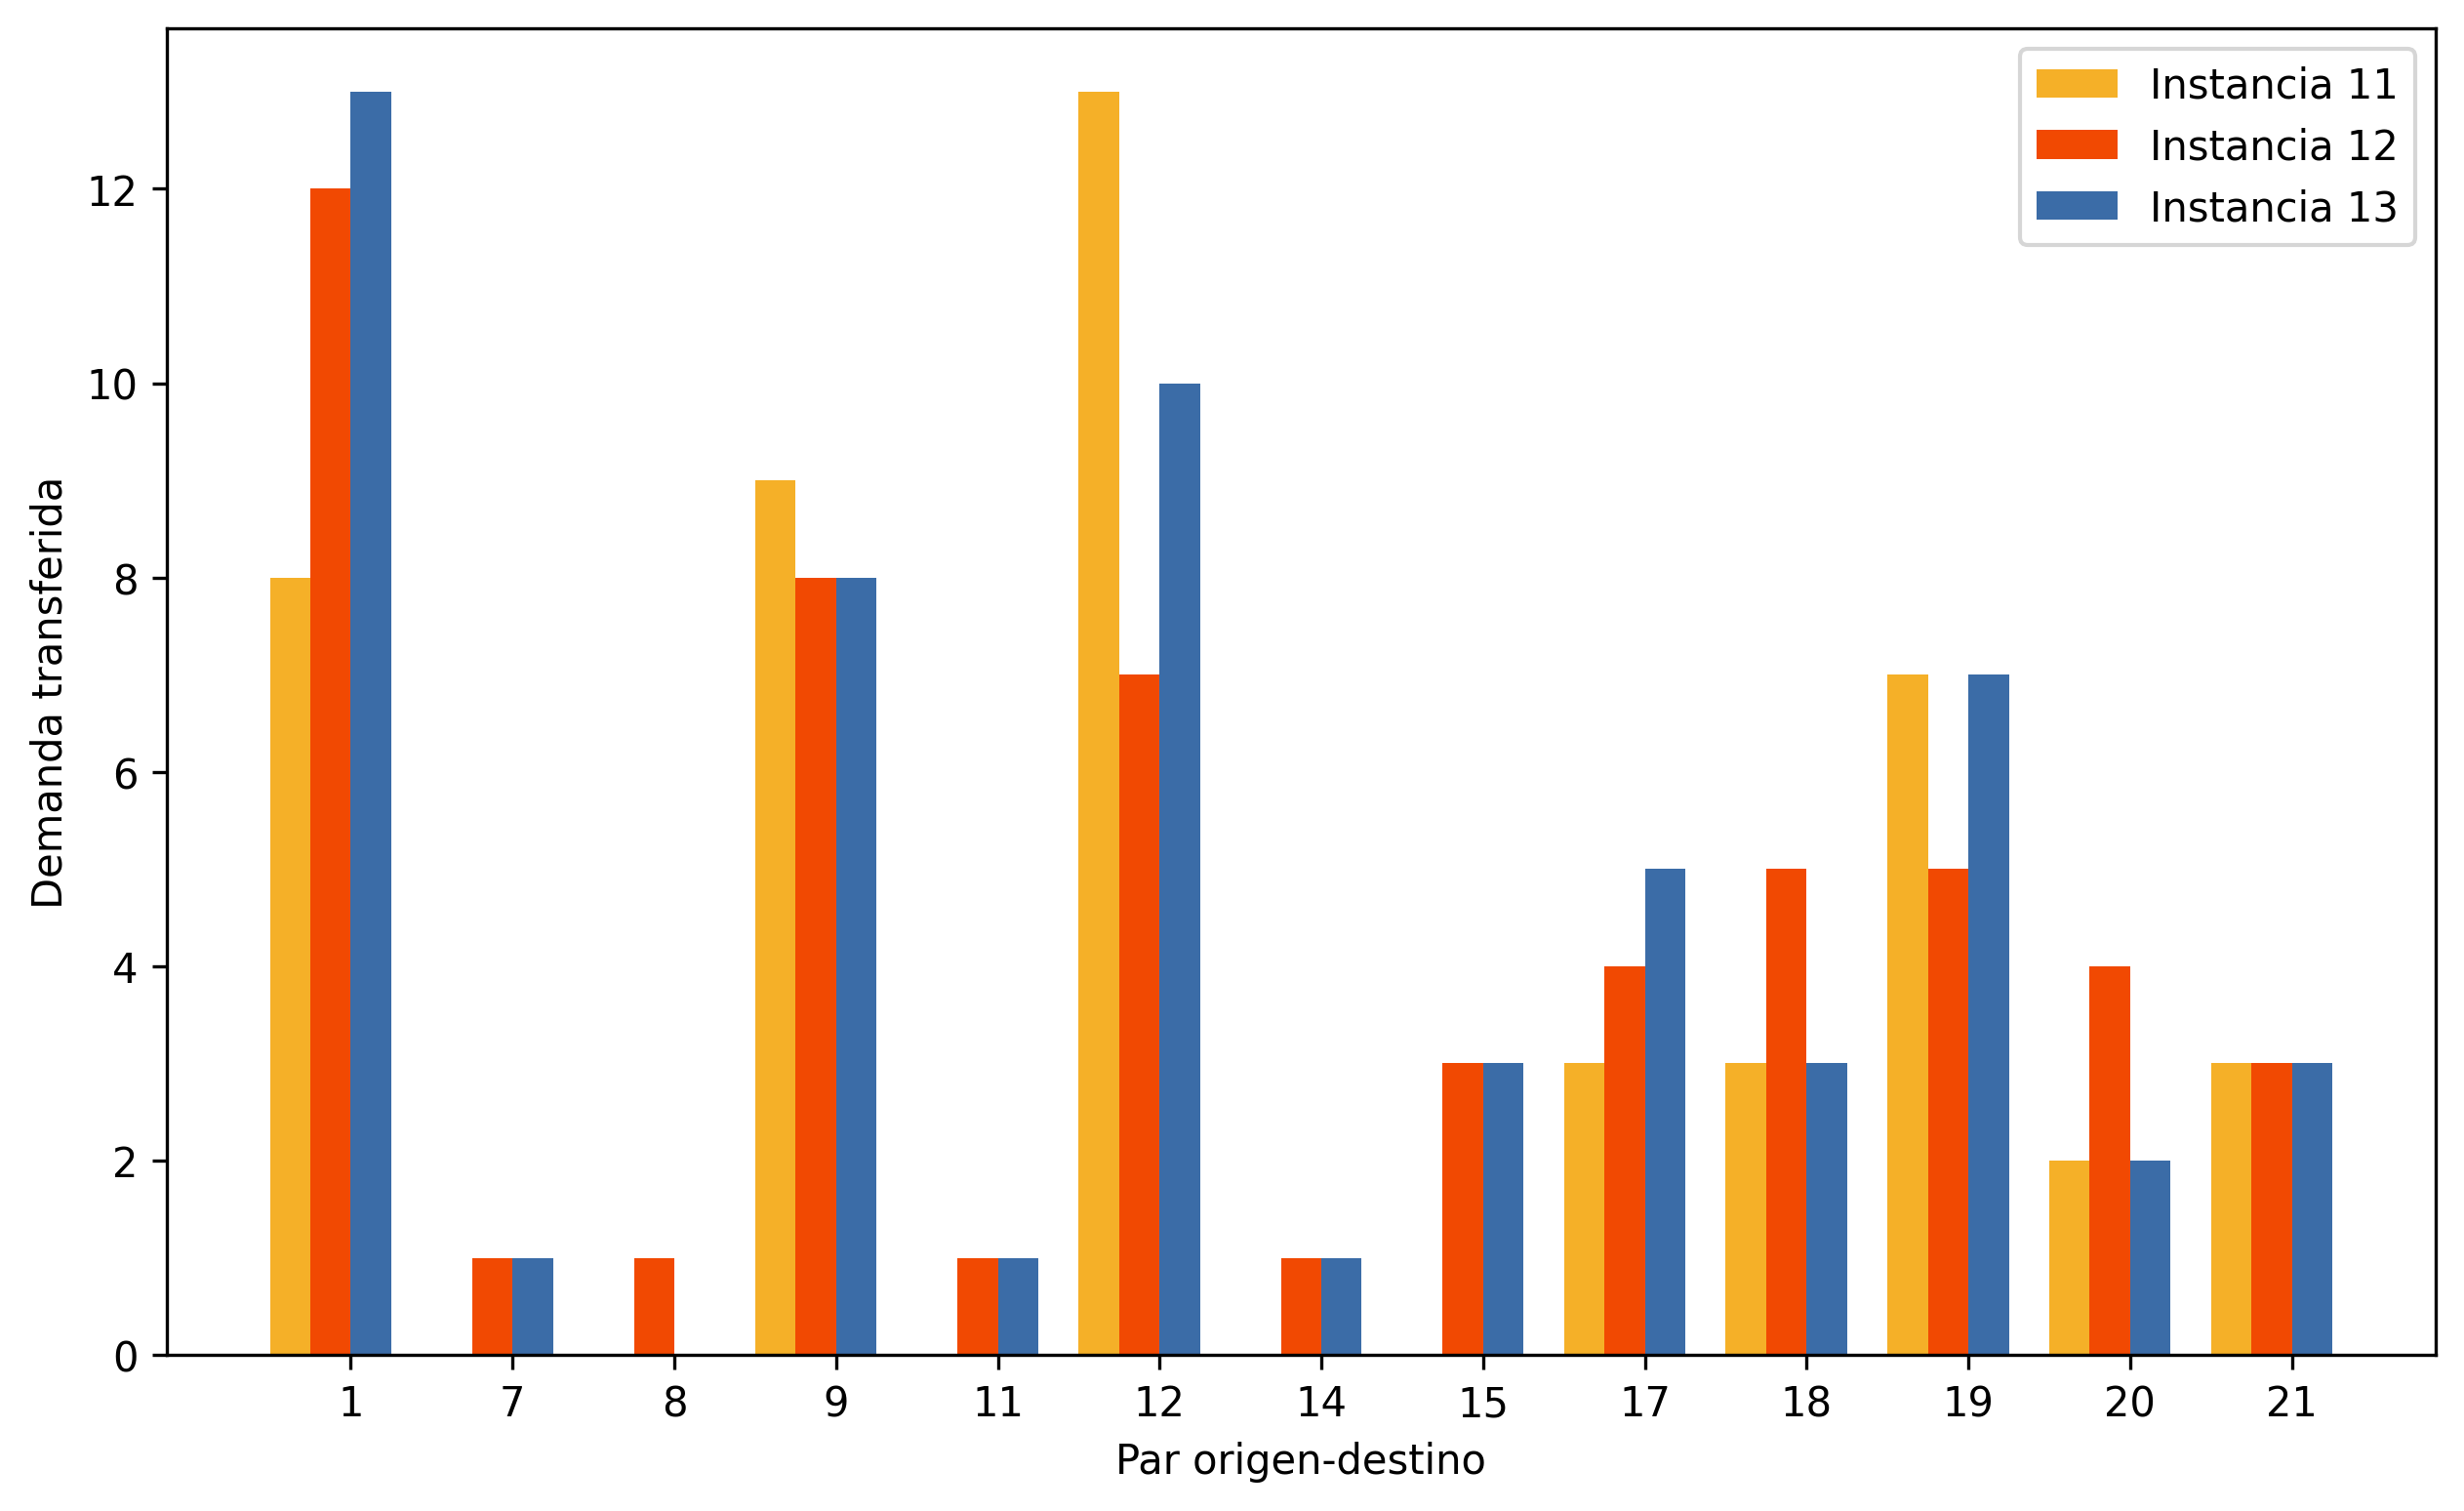
\includegraphics[width=8cm]{../resources/sensibility_case_study_demand.png}
    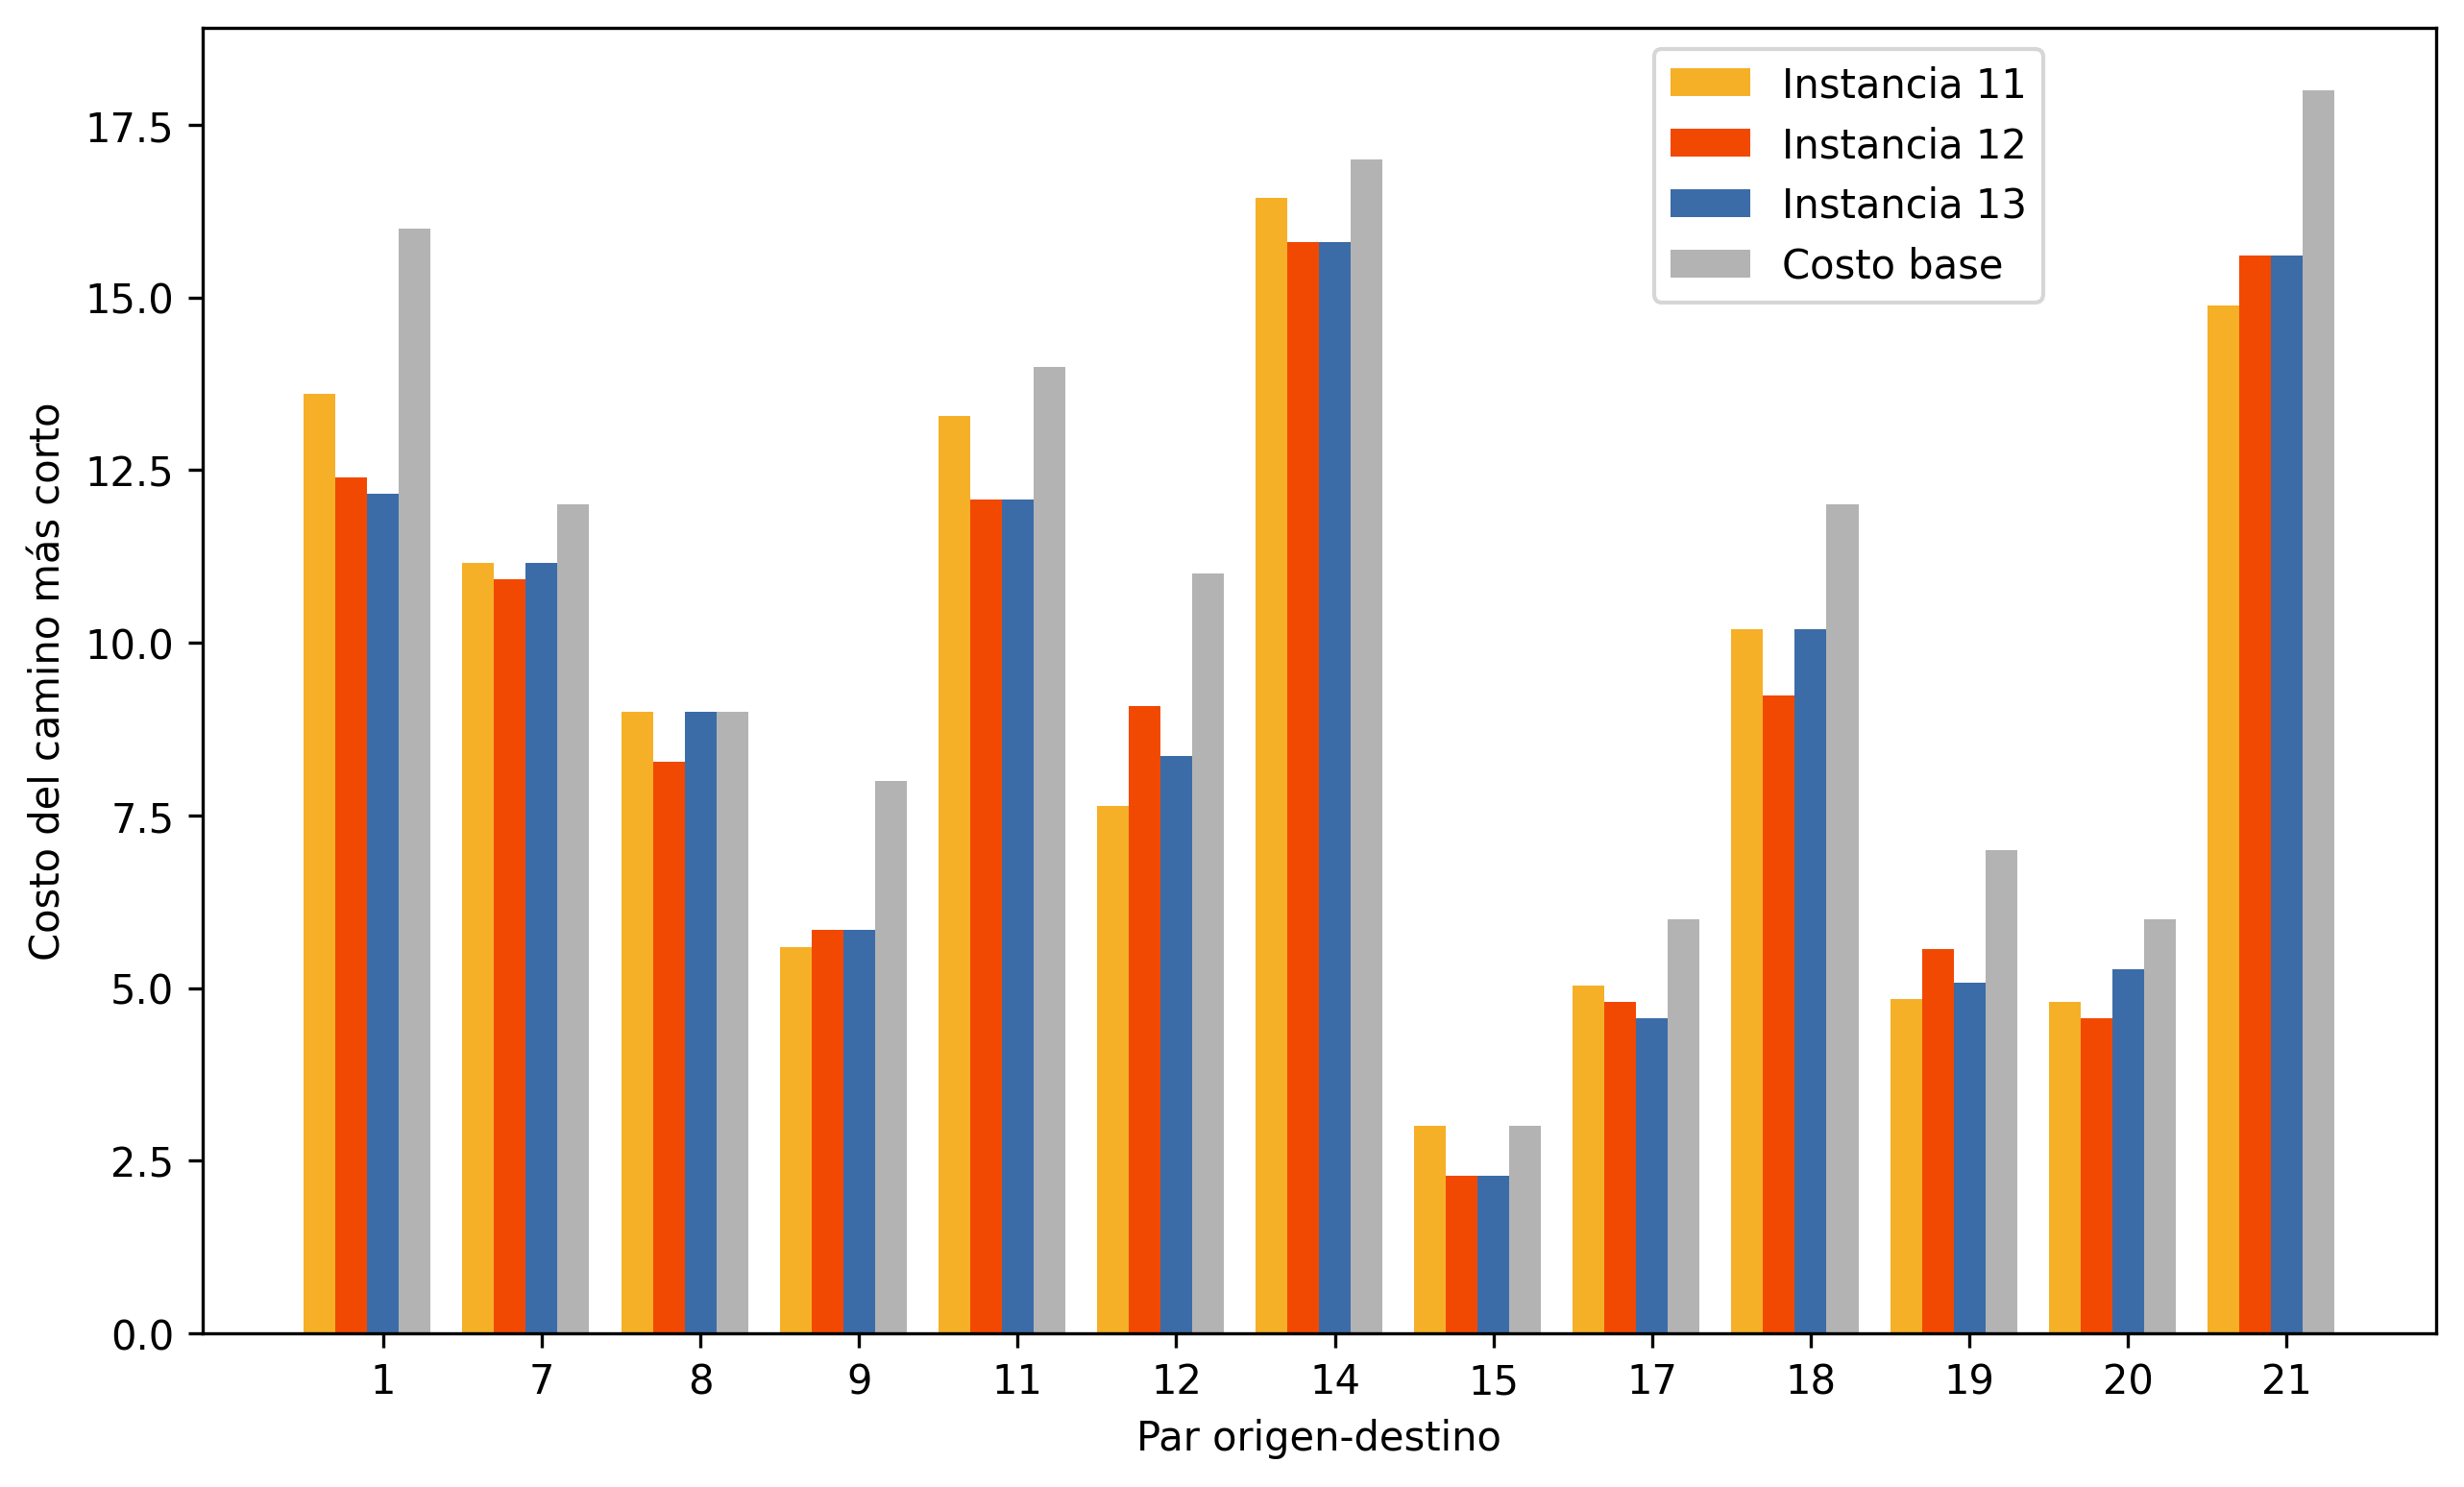
\includegraphics[width=8cm]{../resources/sensibility_case_study_shortest_paths.png}
    \caption{Demanda transferida y costo del camino más corto para los pares origen-destino para los cuales hubo demanda transferida. Los pares origen-destino se numeran de acuerdo a la tabla (\ref{table:siouxfallsdemanddata}) en el apéndice. Los costos de los caminos más cortos se comparan contra el costo base que es aquel sobre la red en la cual no hay ningún tipo de infraestructura construida.}
    \label{fig:sensibilitybyodpair_11_12_13}
  \end{figure}

  \begin{figure}[h!]
    \centering
    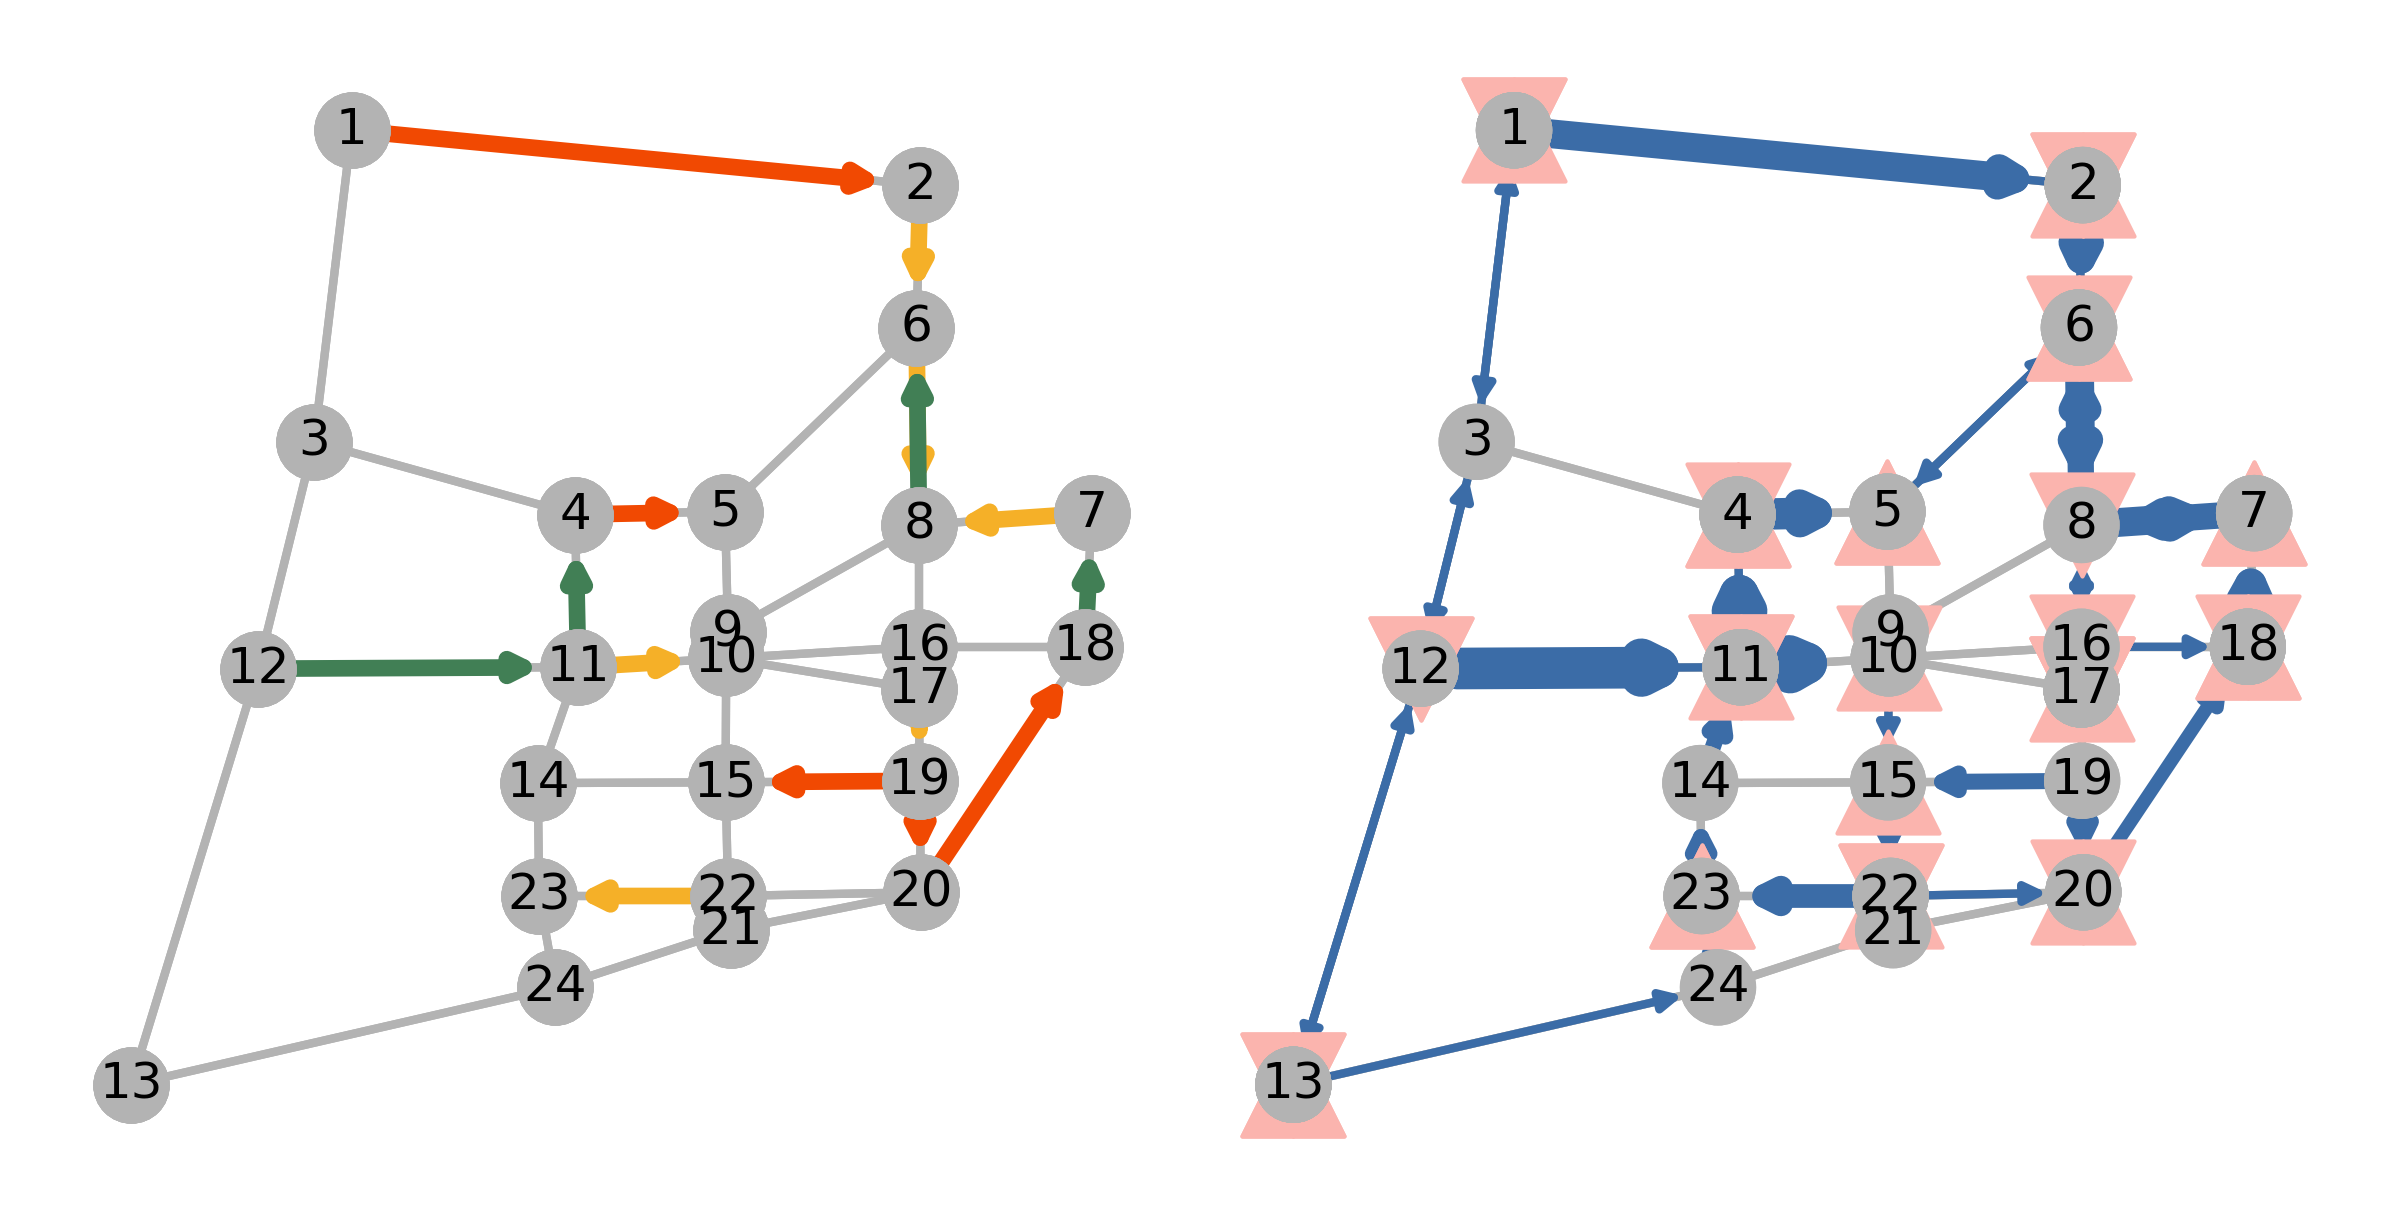
\includegraphics[width=10cm]{../resources/sioux_falls_0.4_budget_factor_linear_5_breakpoints.png}
    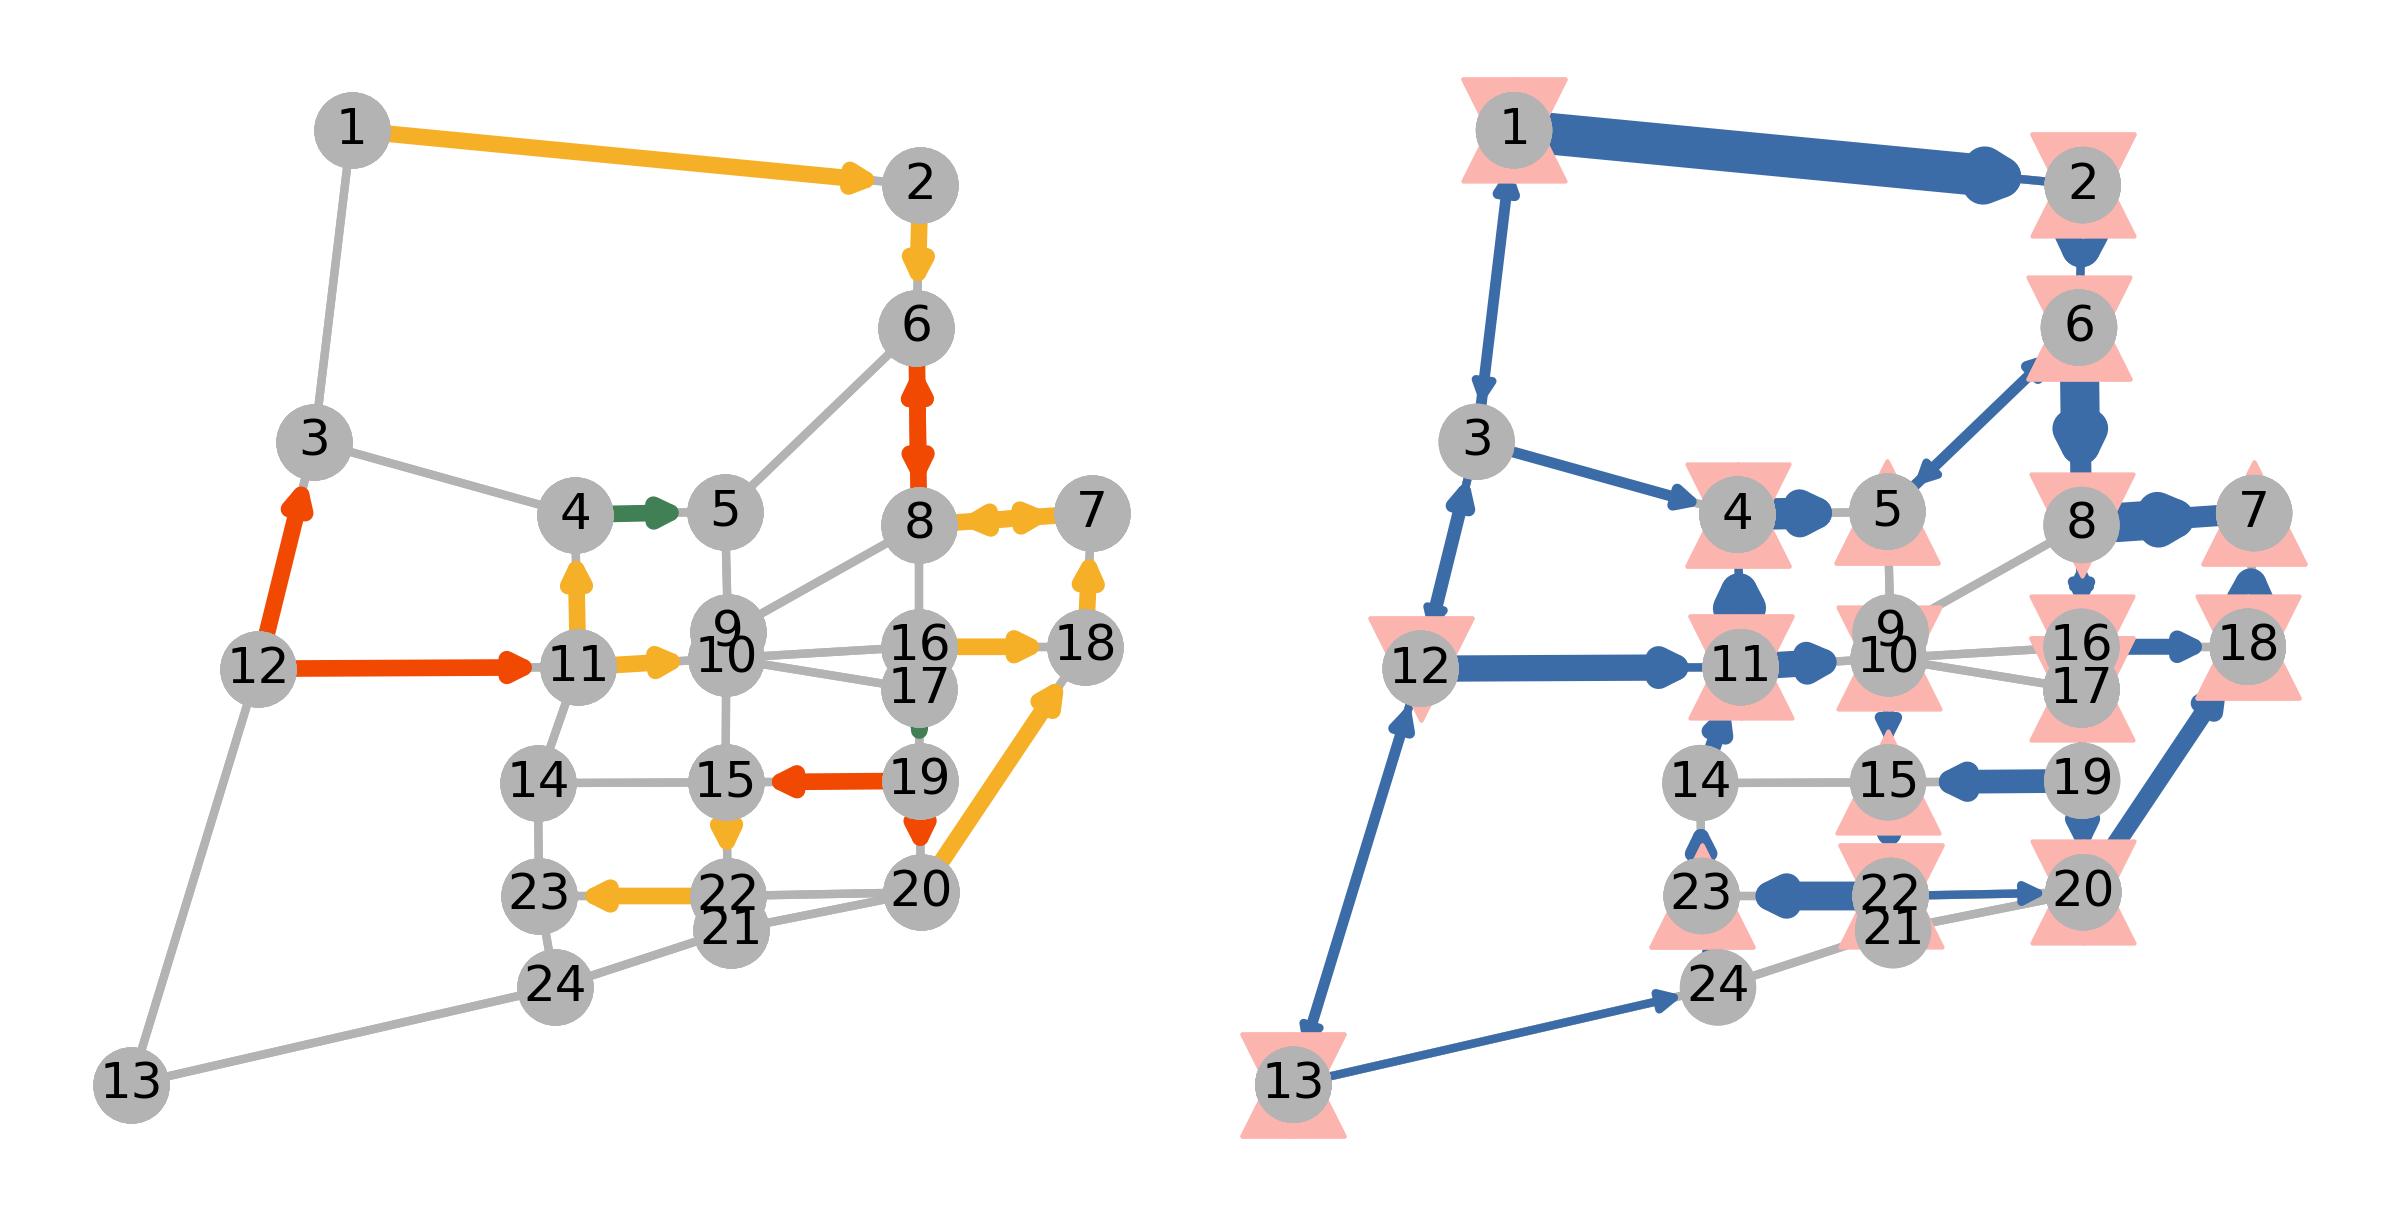
\includegraphics[width=10cm]{../resources/sioux_falls_0.4_budget_factor_linear_20_breakpoints.png}
    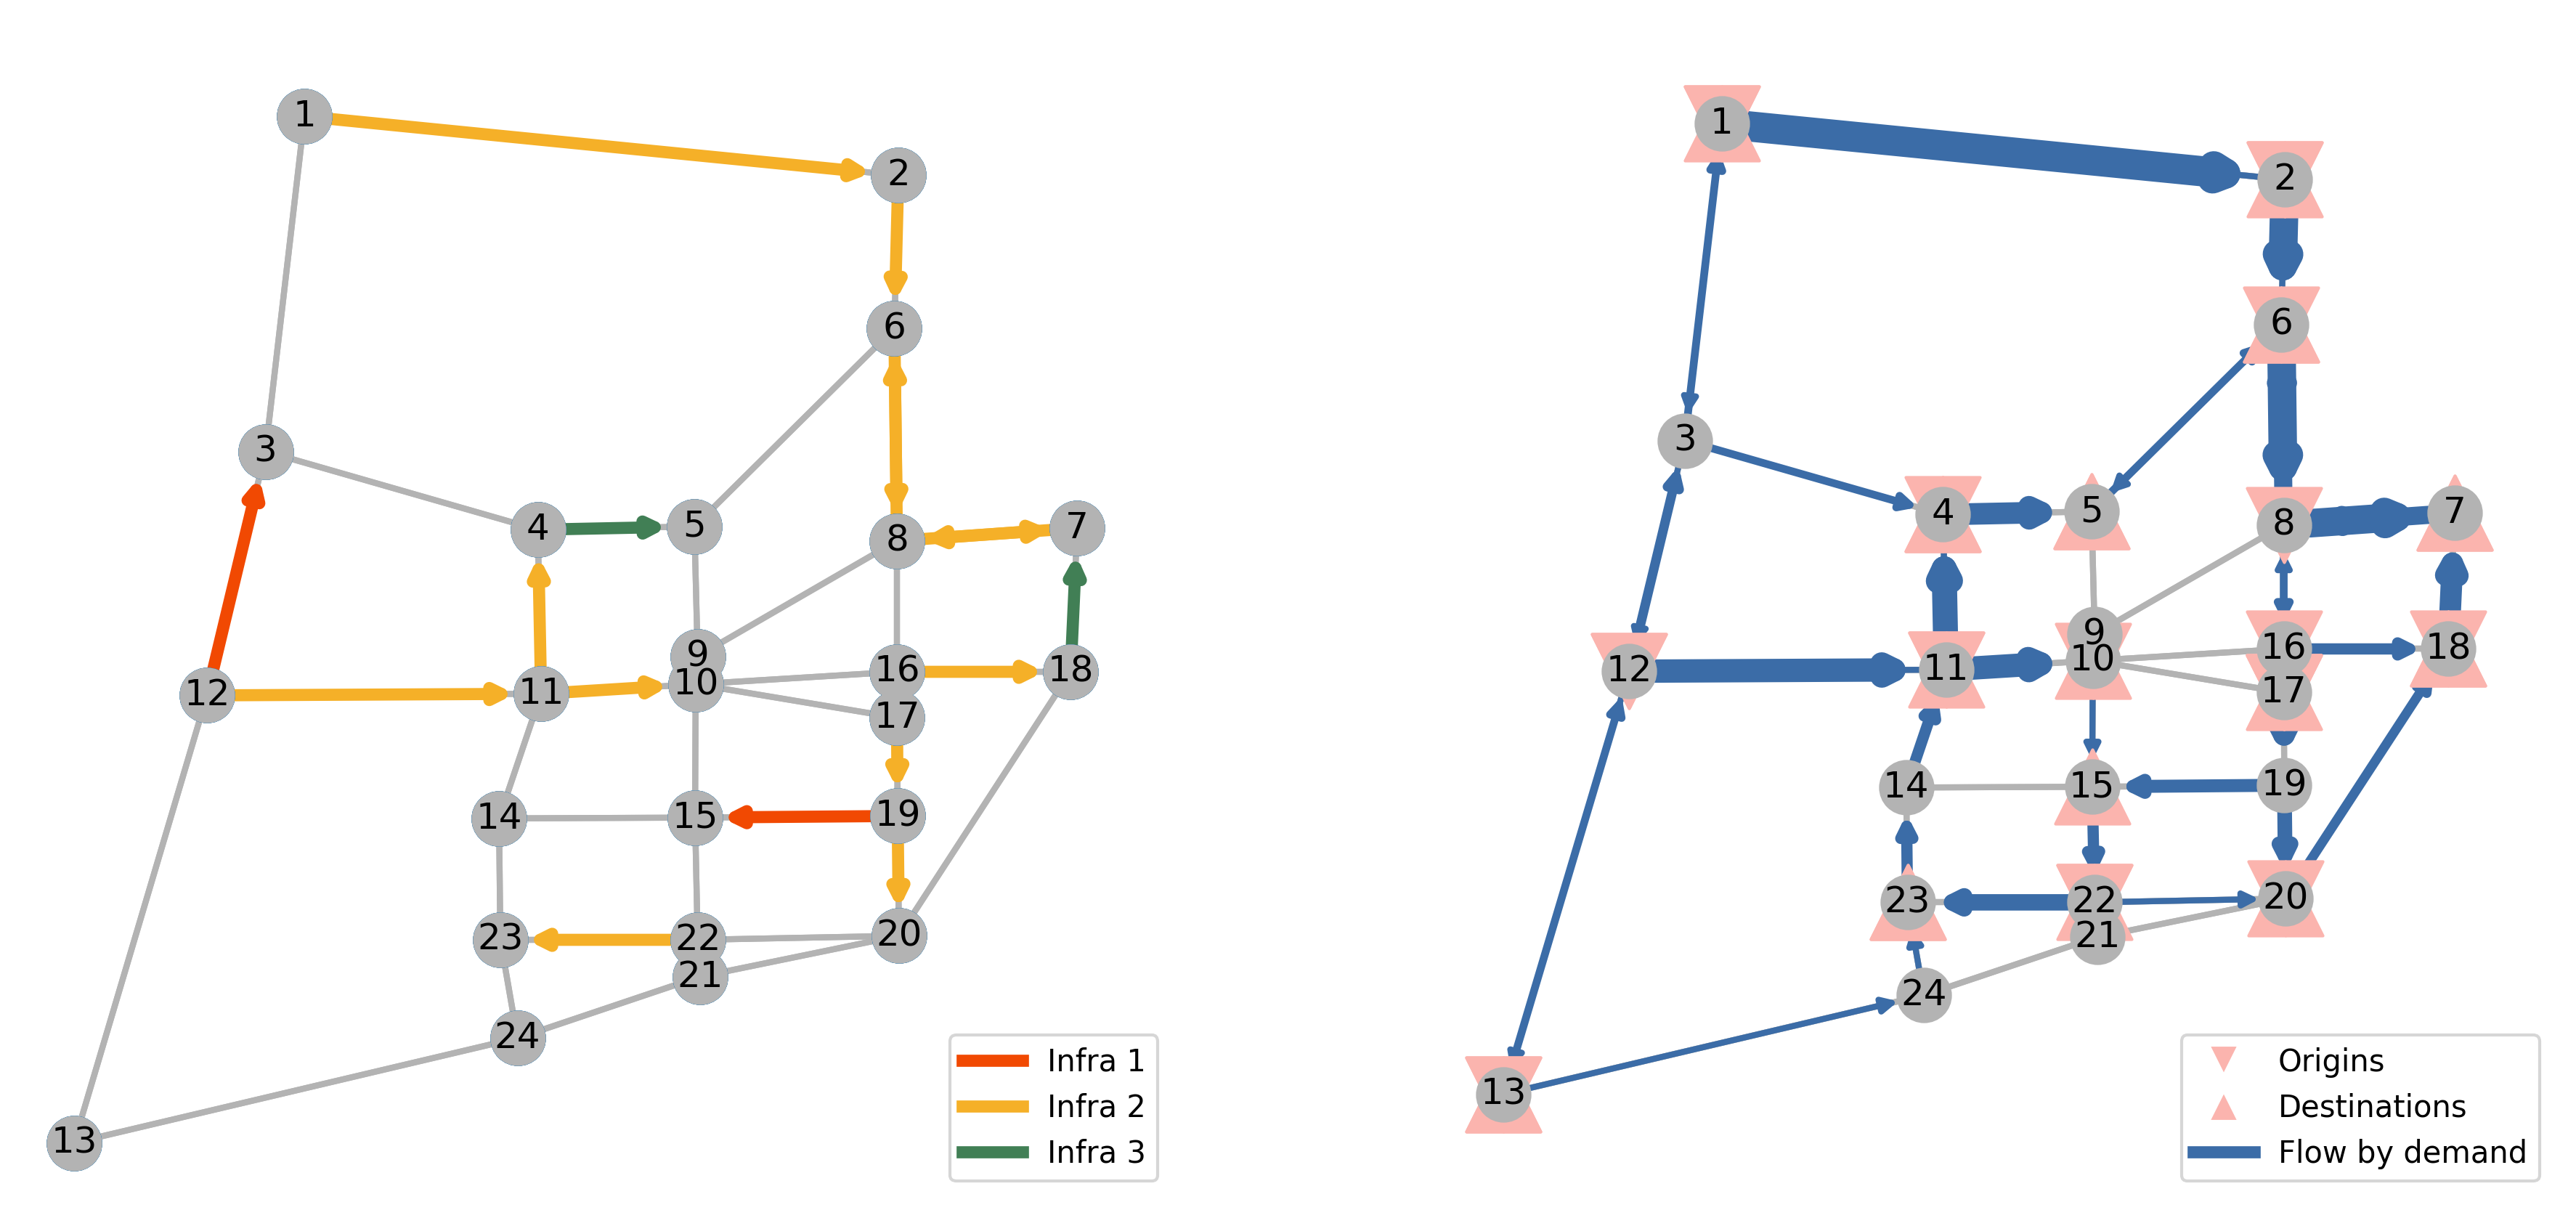
\includegraphics[width=10cm]{../resources/sioux_falls_0.4_budget_factor_linear_50_breakpoints.png}
    \caption{De arriba hacia abajo, instancia 11, 12 y 13. A la izquierda se muestran las ubicaciones de cada tipo de infraestructura. A la derecha los flujos para cada arco considerando el acumulado de demanda de cada par origen-destino que pasaría sobre ellos.}
    \label{fig:sensibilityinstance11_12_13}
  \end{figure}

  \begin{figure}[h!]
    \centering
    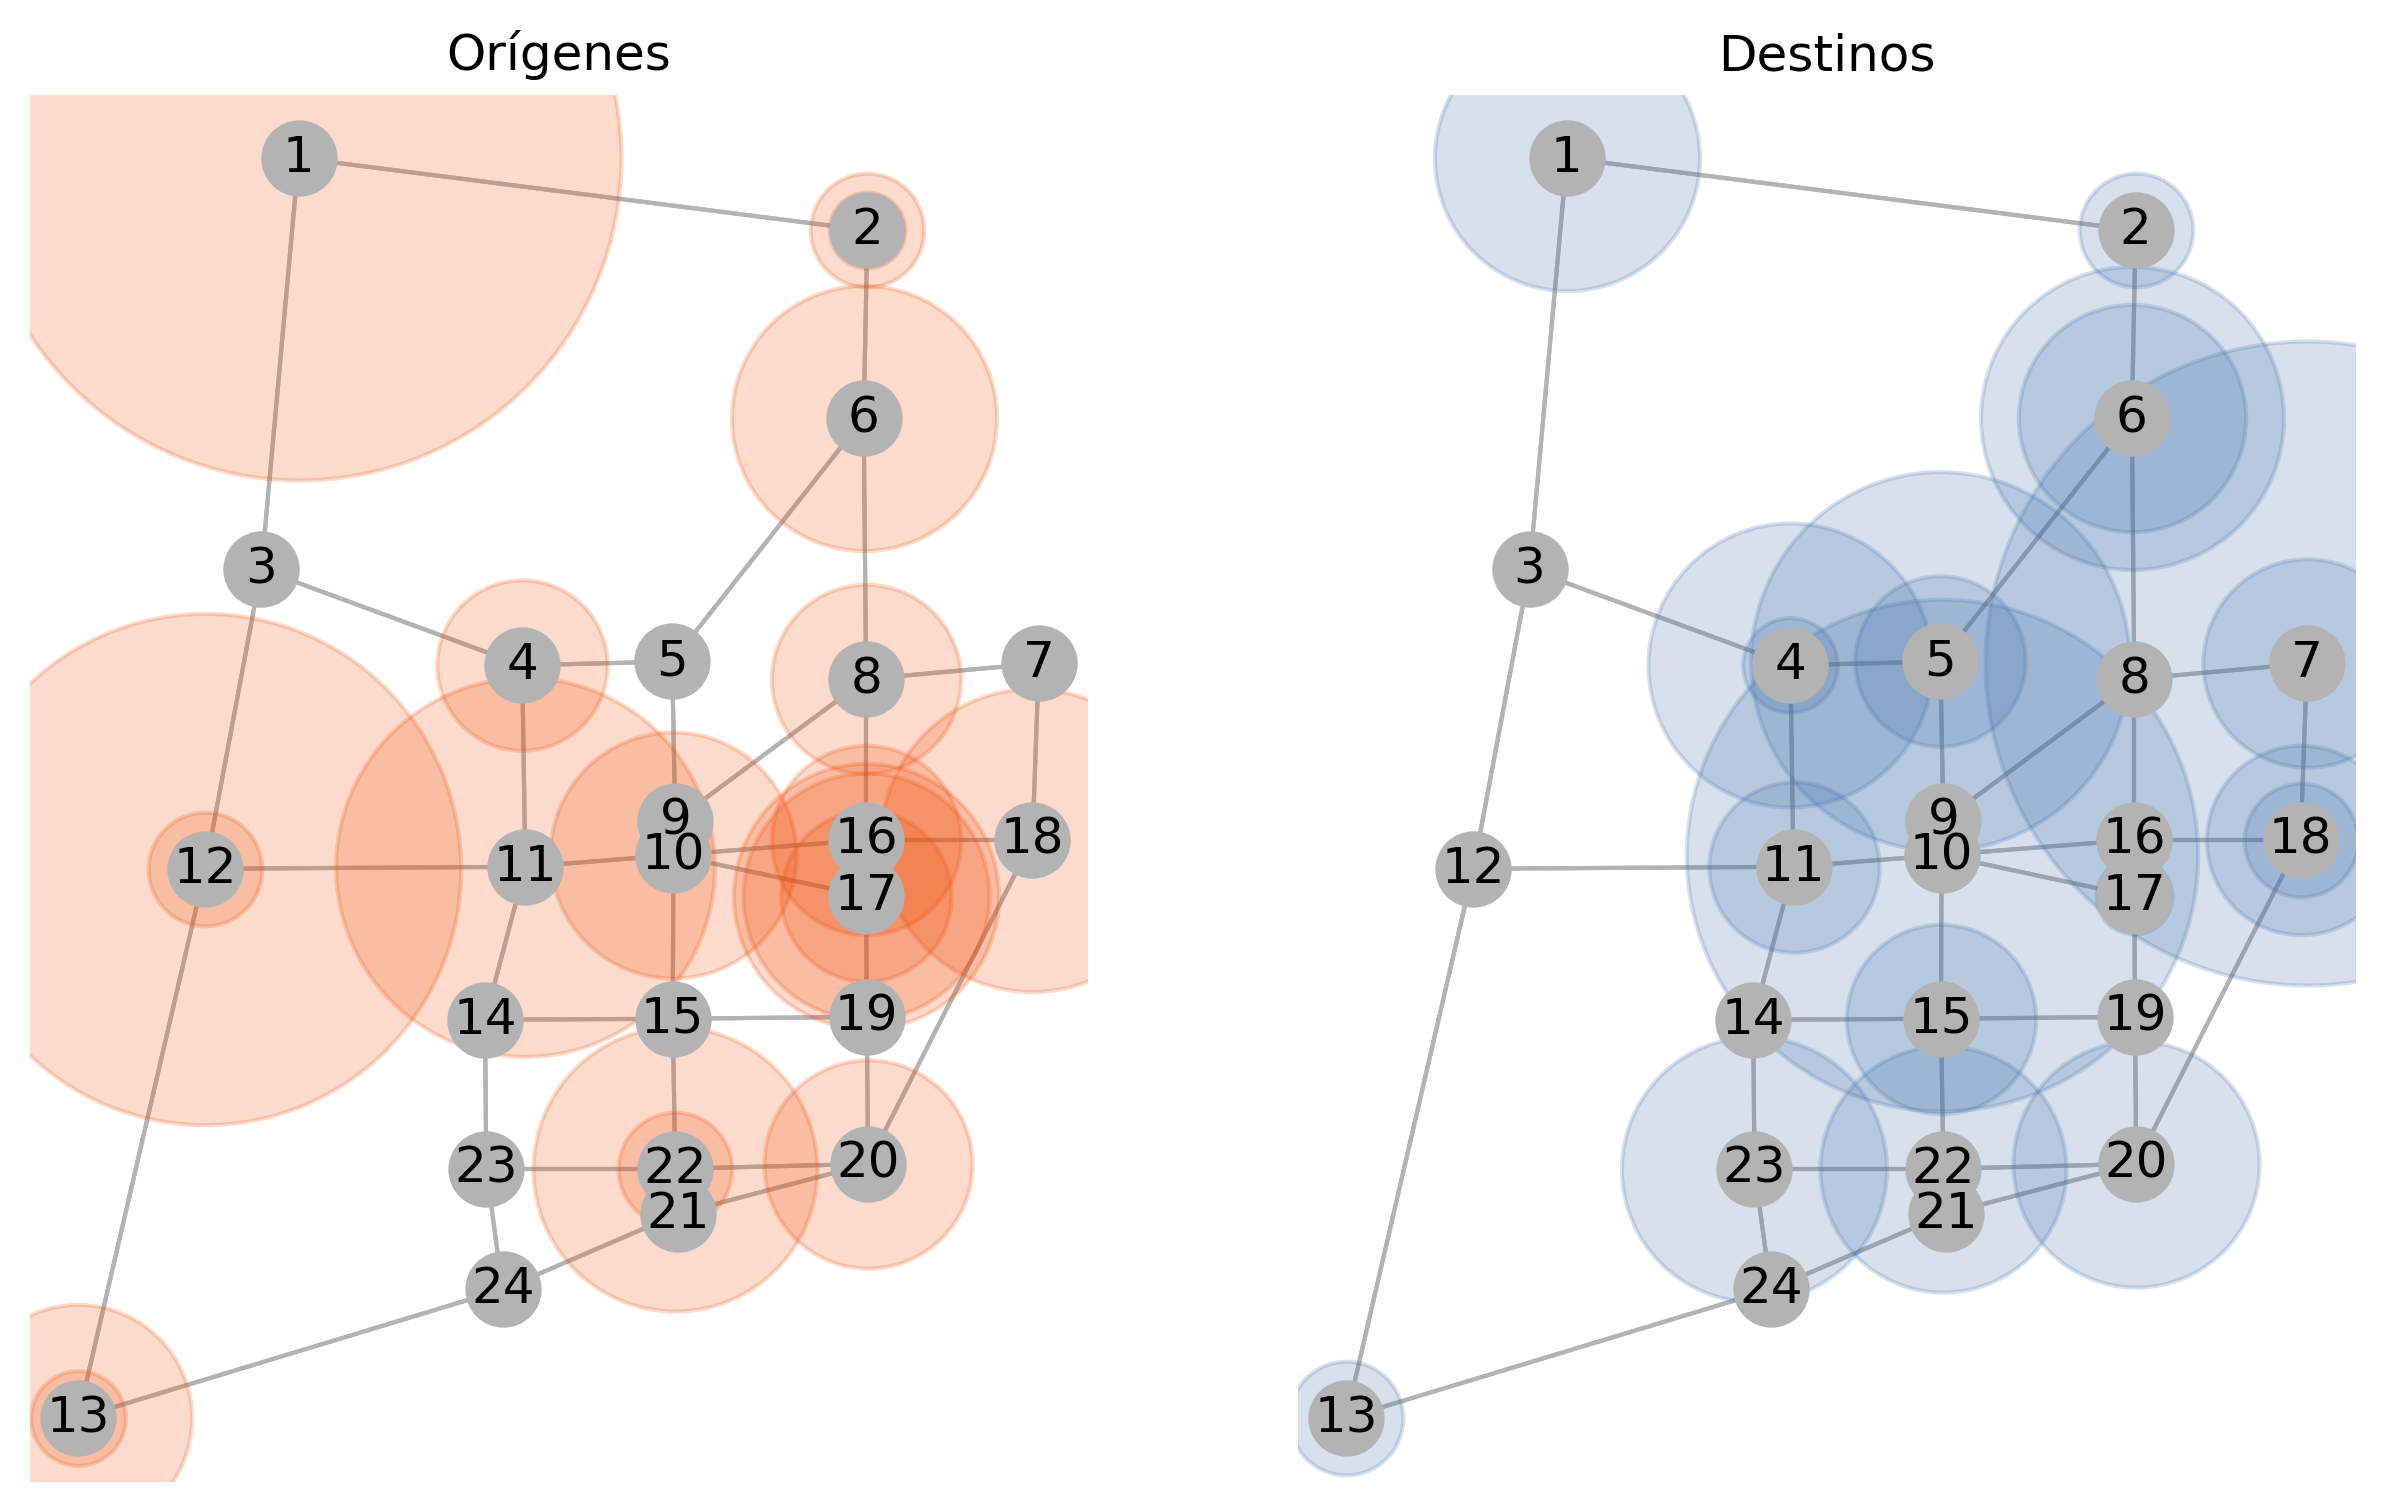
\includegraphics[width=6cm]{../resources/sioux_falls_demand.png}
    \caption{Visualización de la distribución del pares origen y destino junto a su valor de demanda representado por el tamaño de los círculos para la instancia de Sioux-Falls.}
    \label{fig:sioux_falls_demand}
  \end{figure}

  \FloatBarrier
  \subsection{Aplicación sobre una instancia realista}

  Como prueba final, utilizamos una instancia de la ciudad de Montevideo de manera de poder analizar la aplicación práctica del problema sobre datos familiares y realistas. Los datos de la instancia provienen de una red sobre una zonificación de la ciudad y un estudio del comportamiento de la demanda TODO: referencias que resulta en un grafo de 136 nodos y 636 arcos. Respecto a la demanda, consideramos un conjunto de 734 pares origen-destino compuesto por aquellos que distan a menos de 5 km de distancia euclídea entre ellos y cuya demanda es significativa, entendido como mayor al 10\% del valor de demanda más alto. Encontramos que una distancia 5 km en línea recta, y distancia Manhattan máxima de poco mas que 7 km, es un límite razonable para viajes en bicicleta común y eléctricas según \cite{anette2018}, donde se estima una distancia de viaje promedio de 2.6 km y 3 km respectivamente y una distancia máxima para las últimas de 13 km.

  Dado el tamaño de la instancia y los recursos computacionales disponibles decidimos utilizar 4 infraestructuras, incluyendo la base, y 10 puntos de quiebre. Probamos las funciones de transferencia de demanda logística y lineal y tres factores de presupuesto: 40\%, 80\% y 160\%. Las instancias fueron resueltas por el solver CPLEX versión 20.1.0.0, en un CPU Xeon Gold 6138 utilizando hasta 16 hilos y hasta 180 GB de memoria. CPLEX fue configurado para utilizar descomposición de Benders de manera automática lo que nos permitió resolver de manera óptima las instancias estudiadas en unas pocas horas. Vale la pena mencionar que realizamos pruebas utilizando más tipos de infraestructura y mayor cantidad de pares origen-destino pero nos encontramos con limitaciones en los recursos disponibles en términos de memoria o límite de tiempo de ejecución de 5 días.

  El resumen de las ejecuciones se encuentra en la tabla (\ref{table:montevideoexecutions}) y la asignación de presupuesto a infraestructuras en la table (\ref{table:montevideobudgetusage}) y figura (\ref{fig:montevideobudgetusage}).

  \begin{table}[h!]
    \centering
    \caption*{{\bf Resumen de ejecuciones}}
    \begin{tabular}{cccccc}
      \toprule
        Instancia & \shortstack{Factor de \\ presupuesto} & \shortstack{Función de \\ transferencia} & \shortstack{Demanda \\ transferida (\%)} & Gap (\%) & \shortstack{Tiempo \\ ejecución} \\
      \midrule
        1 & 0,4 & lineal & 58,03 & 0,5 & 03:07:23 \\
        2 & 0,4 & logit & 57,31 &  & 00:56:14 \\
        3 & 0,8 & lineal & 77,01 &  & 01:11:09 \\
        4 & 0,8 & logit & 74,90 &  & 00:55:41 \\
        5 & 1,6 & lineal & 94,58 &  & 00:18:55 \\
        6 & 1,6 & logit & 93,63 &  & 00:16:48 \\
      \bottomrule
    \end{tabular}
      \caption{Ejecuciones sobre las instancias resueltas para la red de Montevideo.}\label{table:montevideoexecutions}
  \end{table}

  \begin{figure}[h!]
    \centering
    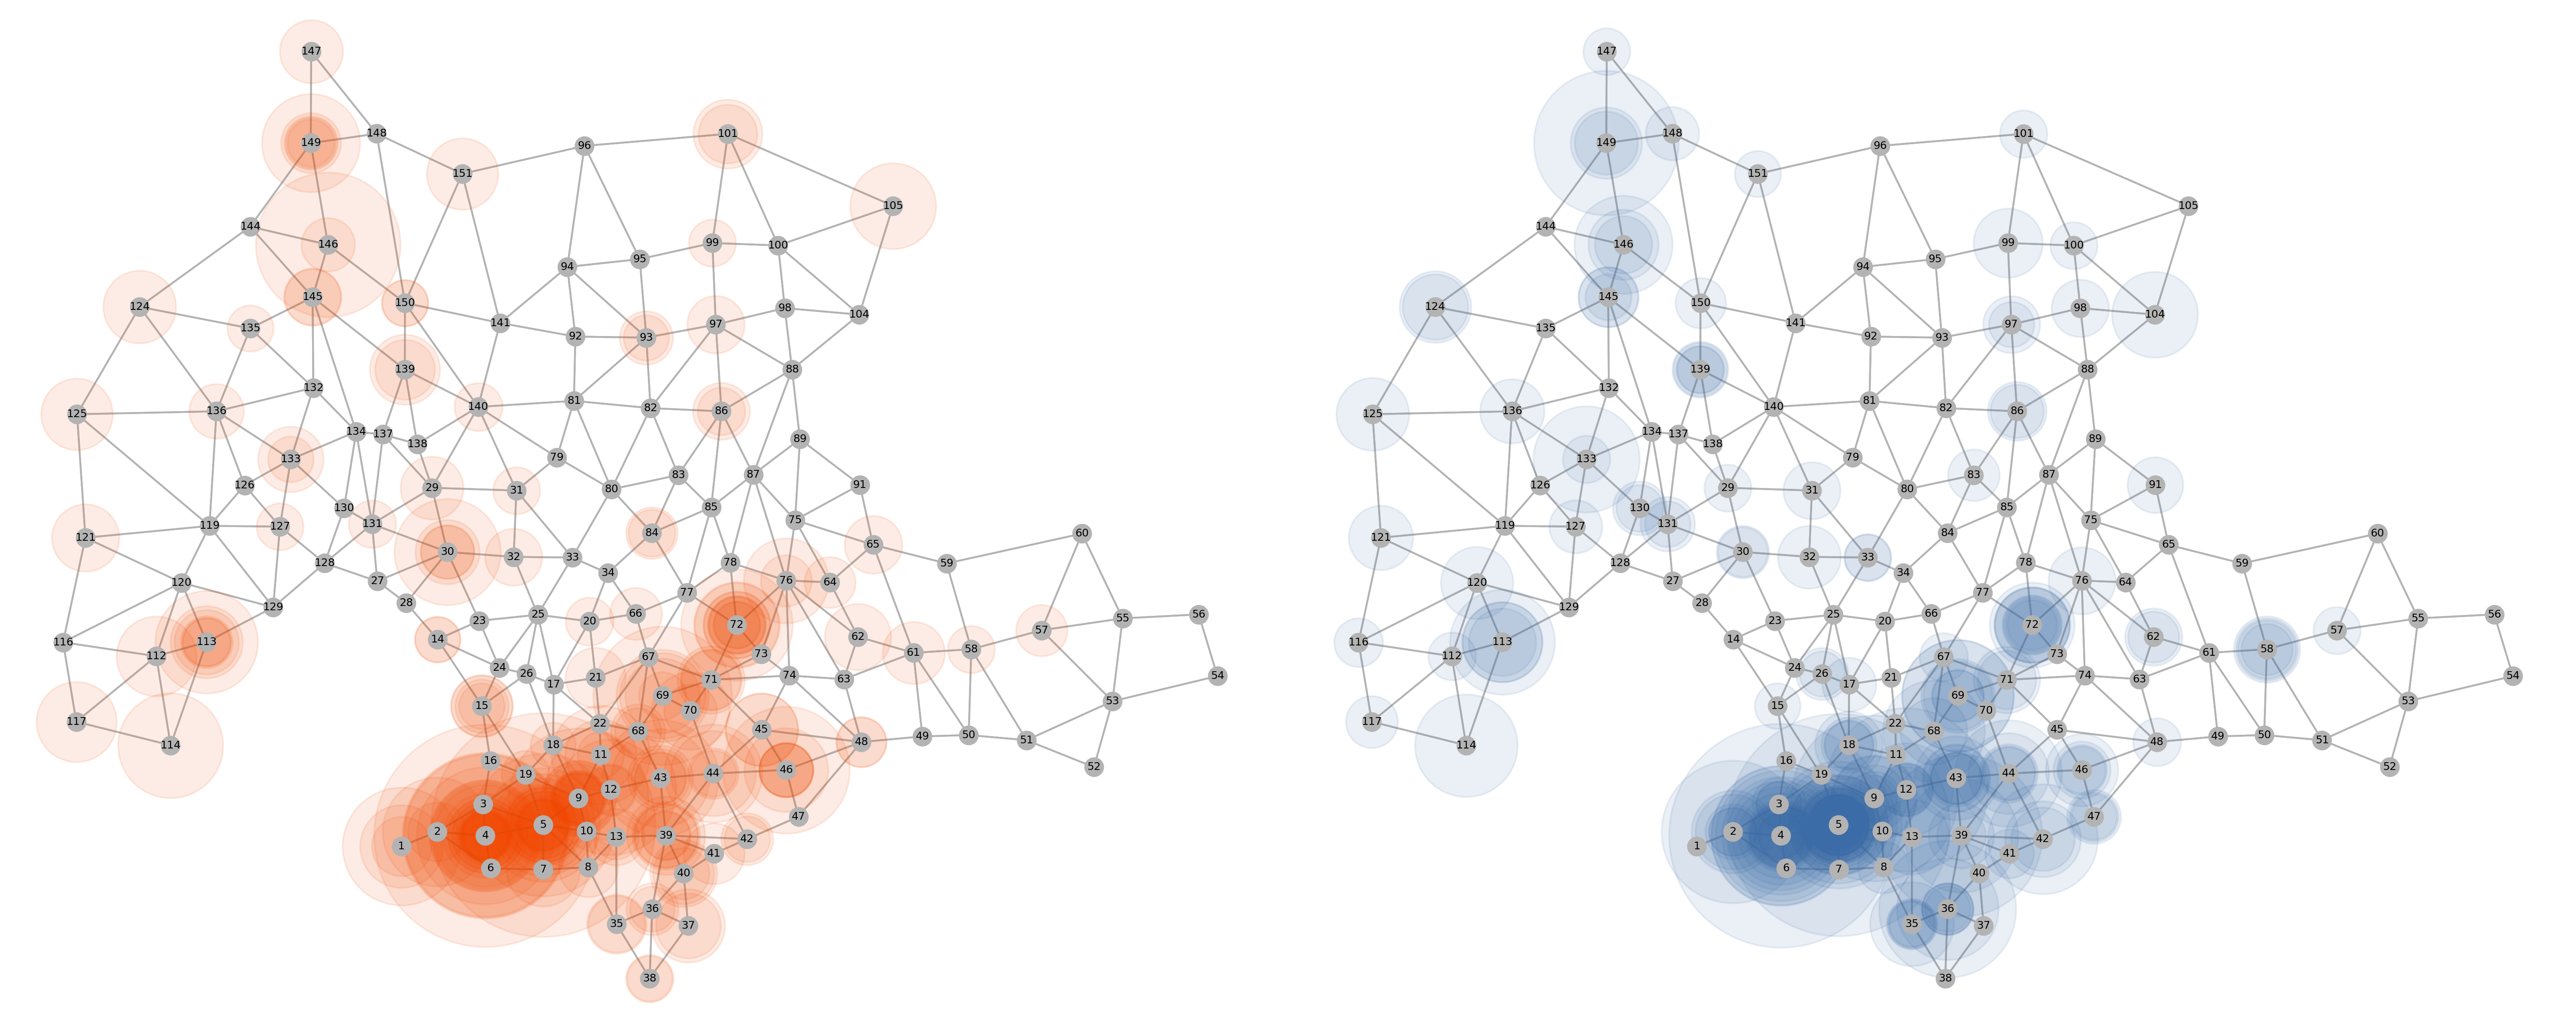
\includegraphics[width=12cm]{../resources/montevideo_demands.png}
      \caption{Representación de demanda por ubicación de origen y destino. Los tamaños de los círculos son proporcionales al valor de demanda. Los primeros 200 pares origen-destino con mayor demanda representados aquí concentran casi el 85\% de la demanda total.}
    \label{fig:montevideodemanddist}
  \end{figure}

  Observamos que los resultados son buenos en términos de demanda transferida para los casos con menor presupuesto en comparación con las instancias de Sioux-Falls. Podemos explicar esto porque la distribución del grueso de la demanda en la red de Montevideo, como se puede ver en la figura (\ref{fig:montevideodemanddist}), se ubica en la misma región de la red. Por lo tanto concentrar la inversión en esa zona produce resultados de amplio impacto.

  Respecto a las infraestructuras construidas, vemos que la función de transferencia de demanda que usemos hace variar la distribución de uso del gasto a igual factor de presupuesto, ver tabla (\ref{table:montevideobudgetusage}) y la figura (\ref{fig:montevideo_instances_infras}) para una representación gráfica. Esto es esperable ya que la función de comportamiento de la demanda dicta que mejoras realizar y con qué criterio. Si consideramos ademas los datos de la tabla (\ref{table:montevideoinfracoverage}) vemos que la función de transferencia lineal induce una utilización que afecta potencialmente a mayor cantidad de pares origen-destino y por lo tanto podría resultar en decisiones que podrían beneficiar a más usuarios que la logística dado que abarca más superficie a expensas de menor calidad en promedio.

  \begin{table}[h!]
    \centering
    \caption*{{\bf Utilización del presupuesto por infraestructura}}
    \begin{tabular}{cccccc}
      \toprule
        Instancia & Presupuesto & \shortstack{Presupuesto \\ utilizado} & Infra 1 (\%) & Infra 2 (\%) & Infra 3 (\%) \\
      \midrule
        1 & 324220,24 & 324092,30 & 0,99 & 27,85 & 71,12 \\
        2 & 324220,24 & 324179,51 &  & 3,47 & 96,52 \\
        3 & 648440,47 & 648362,17 & 0,82 & 28,03 & 71,14 \\
        4 & 648440,47 & 648438,48 & 0,42 & 3,05 & 96,52 \\
        5 & 1296880,95 & 1296657,95 &  & 12,44 & 87,54 \\
        6 & 1296880,95 & 1296747,87 & 0,14 & 2,59 & 97,26 \\
      \bottomrule
    \end{tabular}
      \caption{Porcentaje del presupuesto utilizado por tipo de infraestructura para cada instancia.}\label{table:montevideobudgetusage}
  \end{table}

  \begin{table}[h!]
    \centering
    \caption*{{\bf Cobertura de cada tipo de infraestructura}}
    \begin{tabular}{ccccc}
      \toprule
        Instancia & Infra. 1 (\%) & Infra. 2 (\%) & Infra. 3 (\%) & Total (\%) \\
      \midrule
        1 & 0.39 & 5.57 & 7.11 & 13.07 \\
        2 & 0.0  & 0.69 & 9.65 & 10.34 \\
        3 & 0.65 & 11.21 & 14.22 & 26.09 \\
        4 & 0.33 & 1.22 & 19.30 & 20.86 \\
        5 & 0.0  & 9.95 & 35.01 & 44.96 \\
        6 & 0.21 & 2.07 & 38.90 & 41.19 \\
      \bottomrule
    \end{tabular}
    \caption{Porcentaje del total de caminos cubierto por cada tipo de infraestructura.}
    \label{table:montevideoinfracoverage}
  \end{table}

  \begin{figure}[h!]
    \centering
    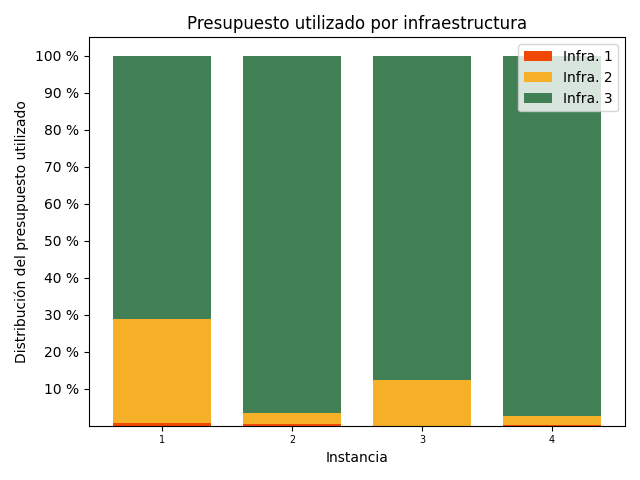
\includegraphics[width=8cm]{../resources/montevideo_budget_usage_by_infra.png}
      \caption{}
    \label{fig:montevideobudgetusage}
  \end{figure}

  \begin{figure}[h!]
    \centering
    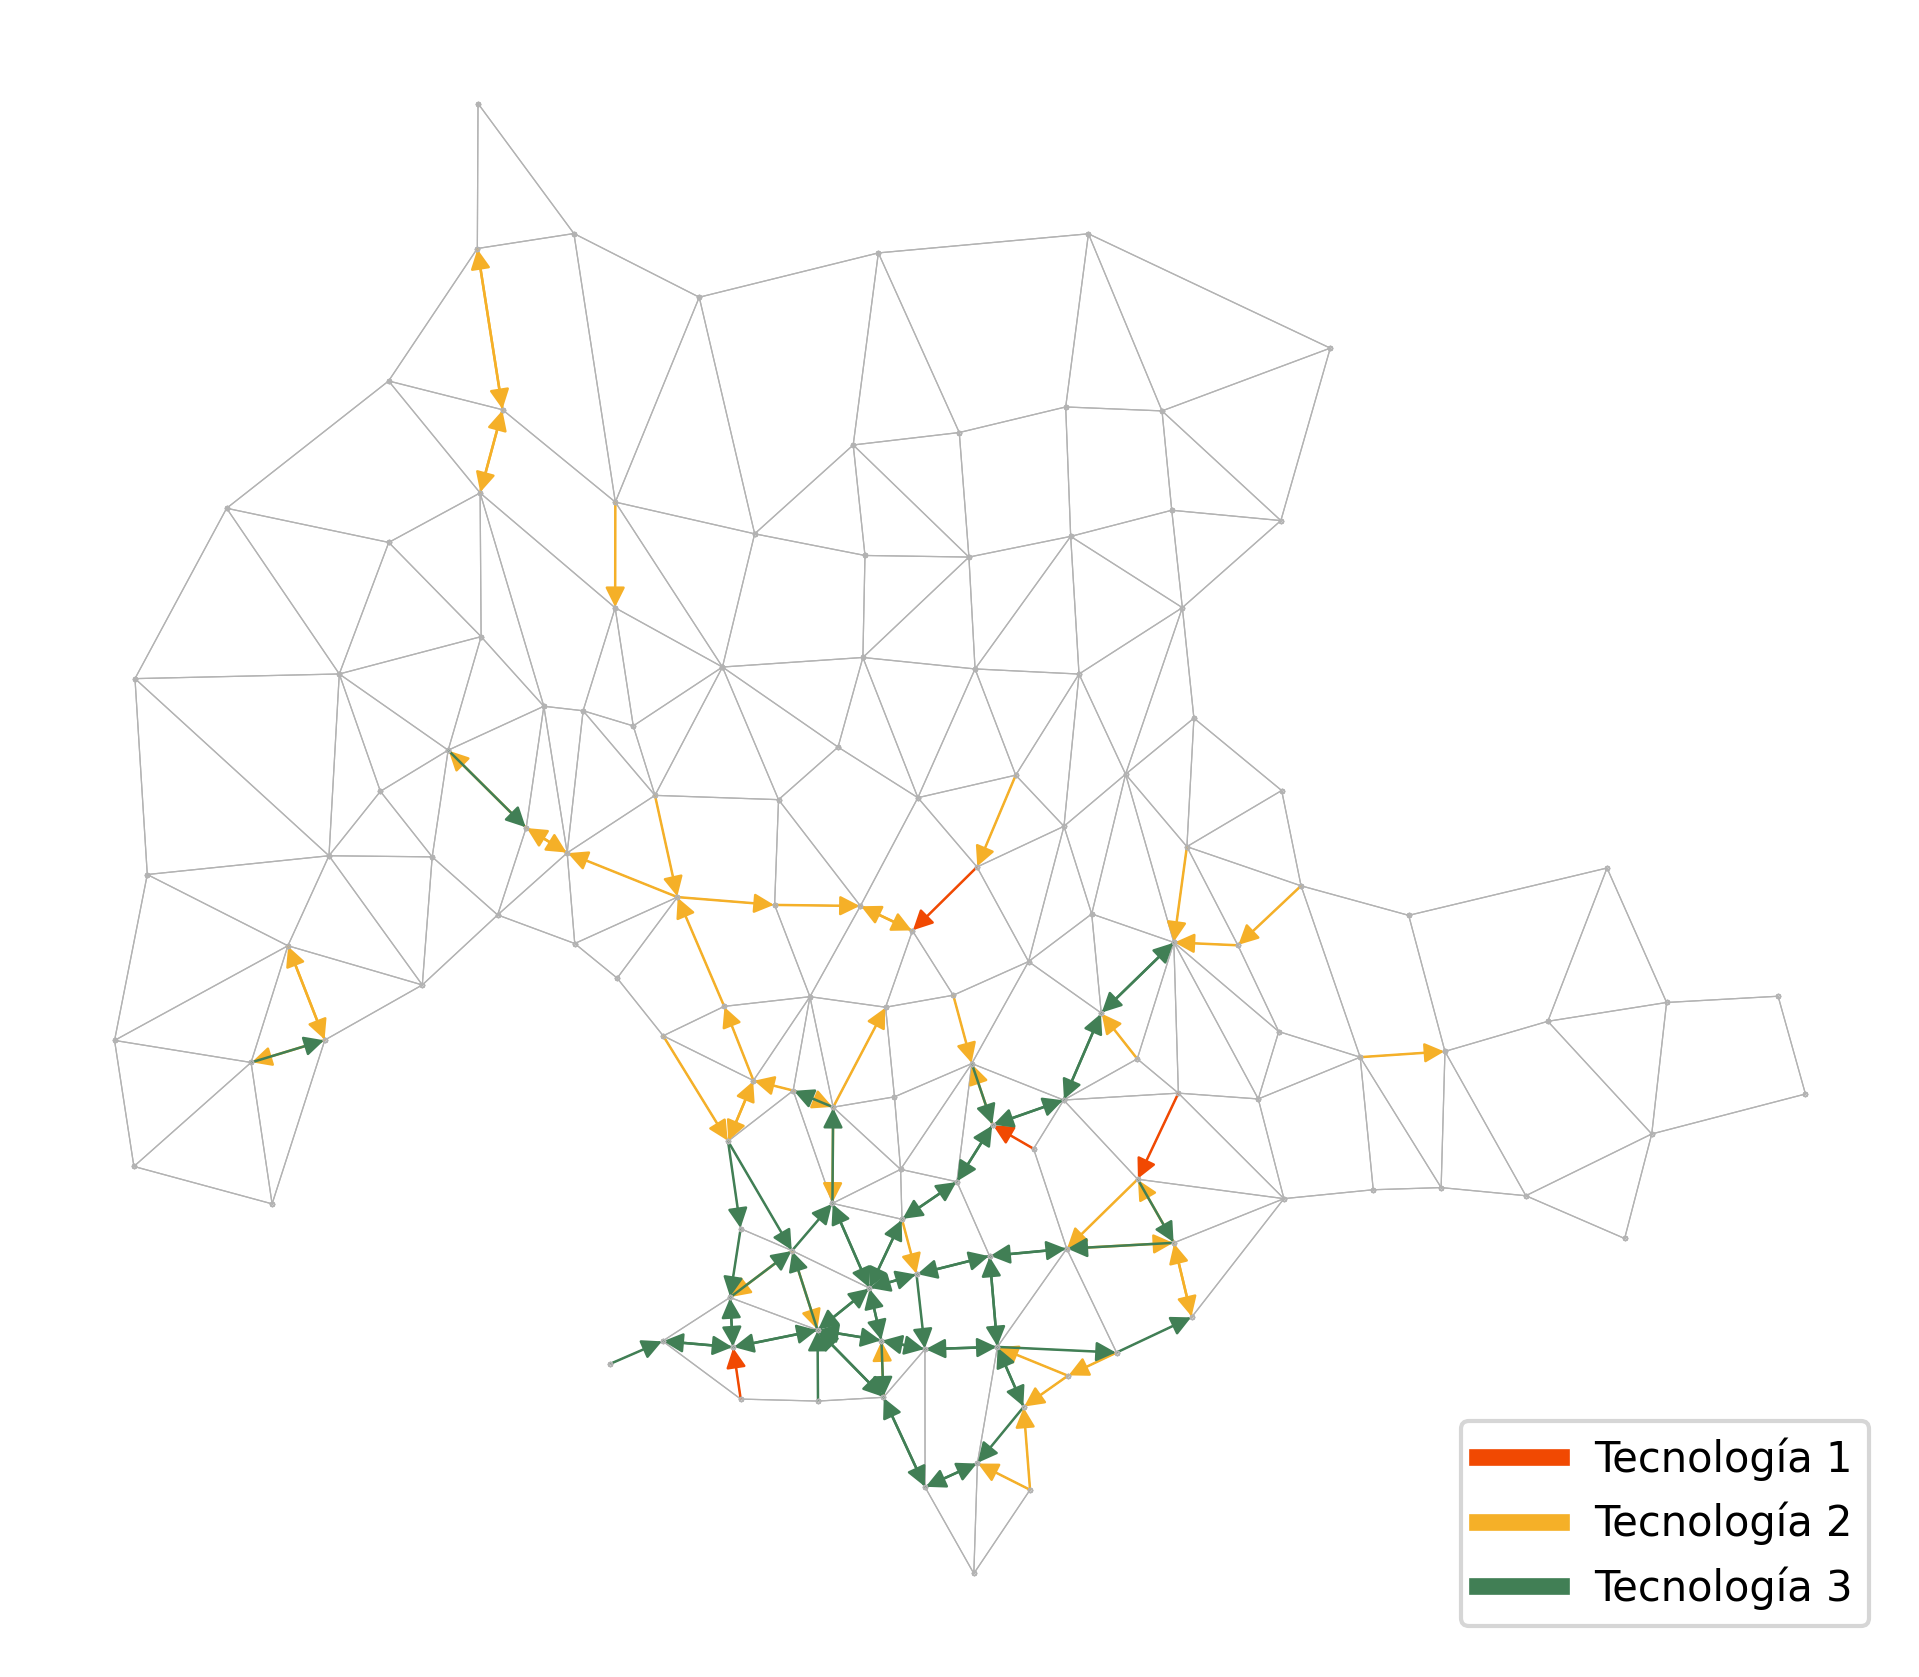
\includegraphics[width=6cm]{../resources/montevideo_d5000.0_linear_0.4_budget_factor.png}
    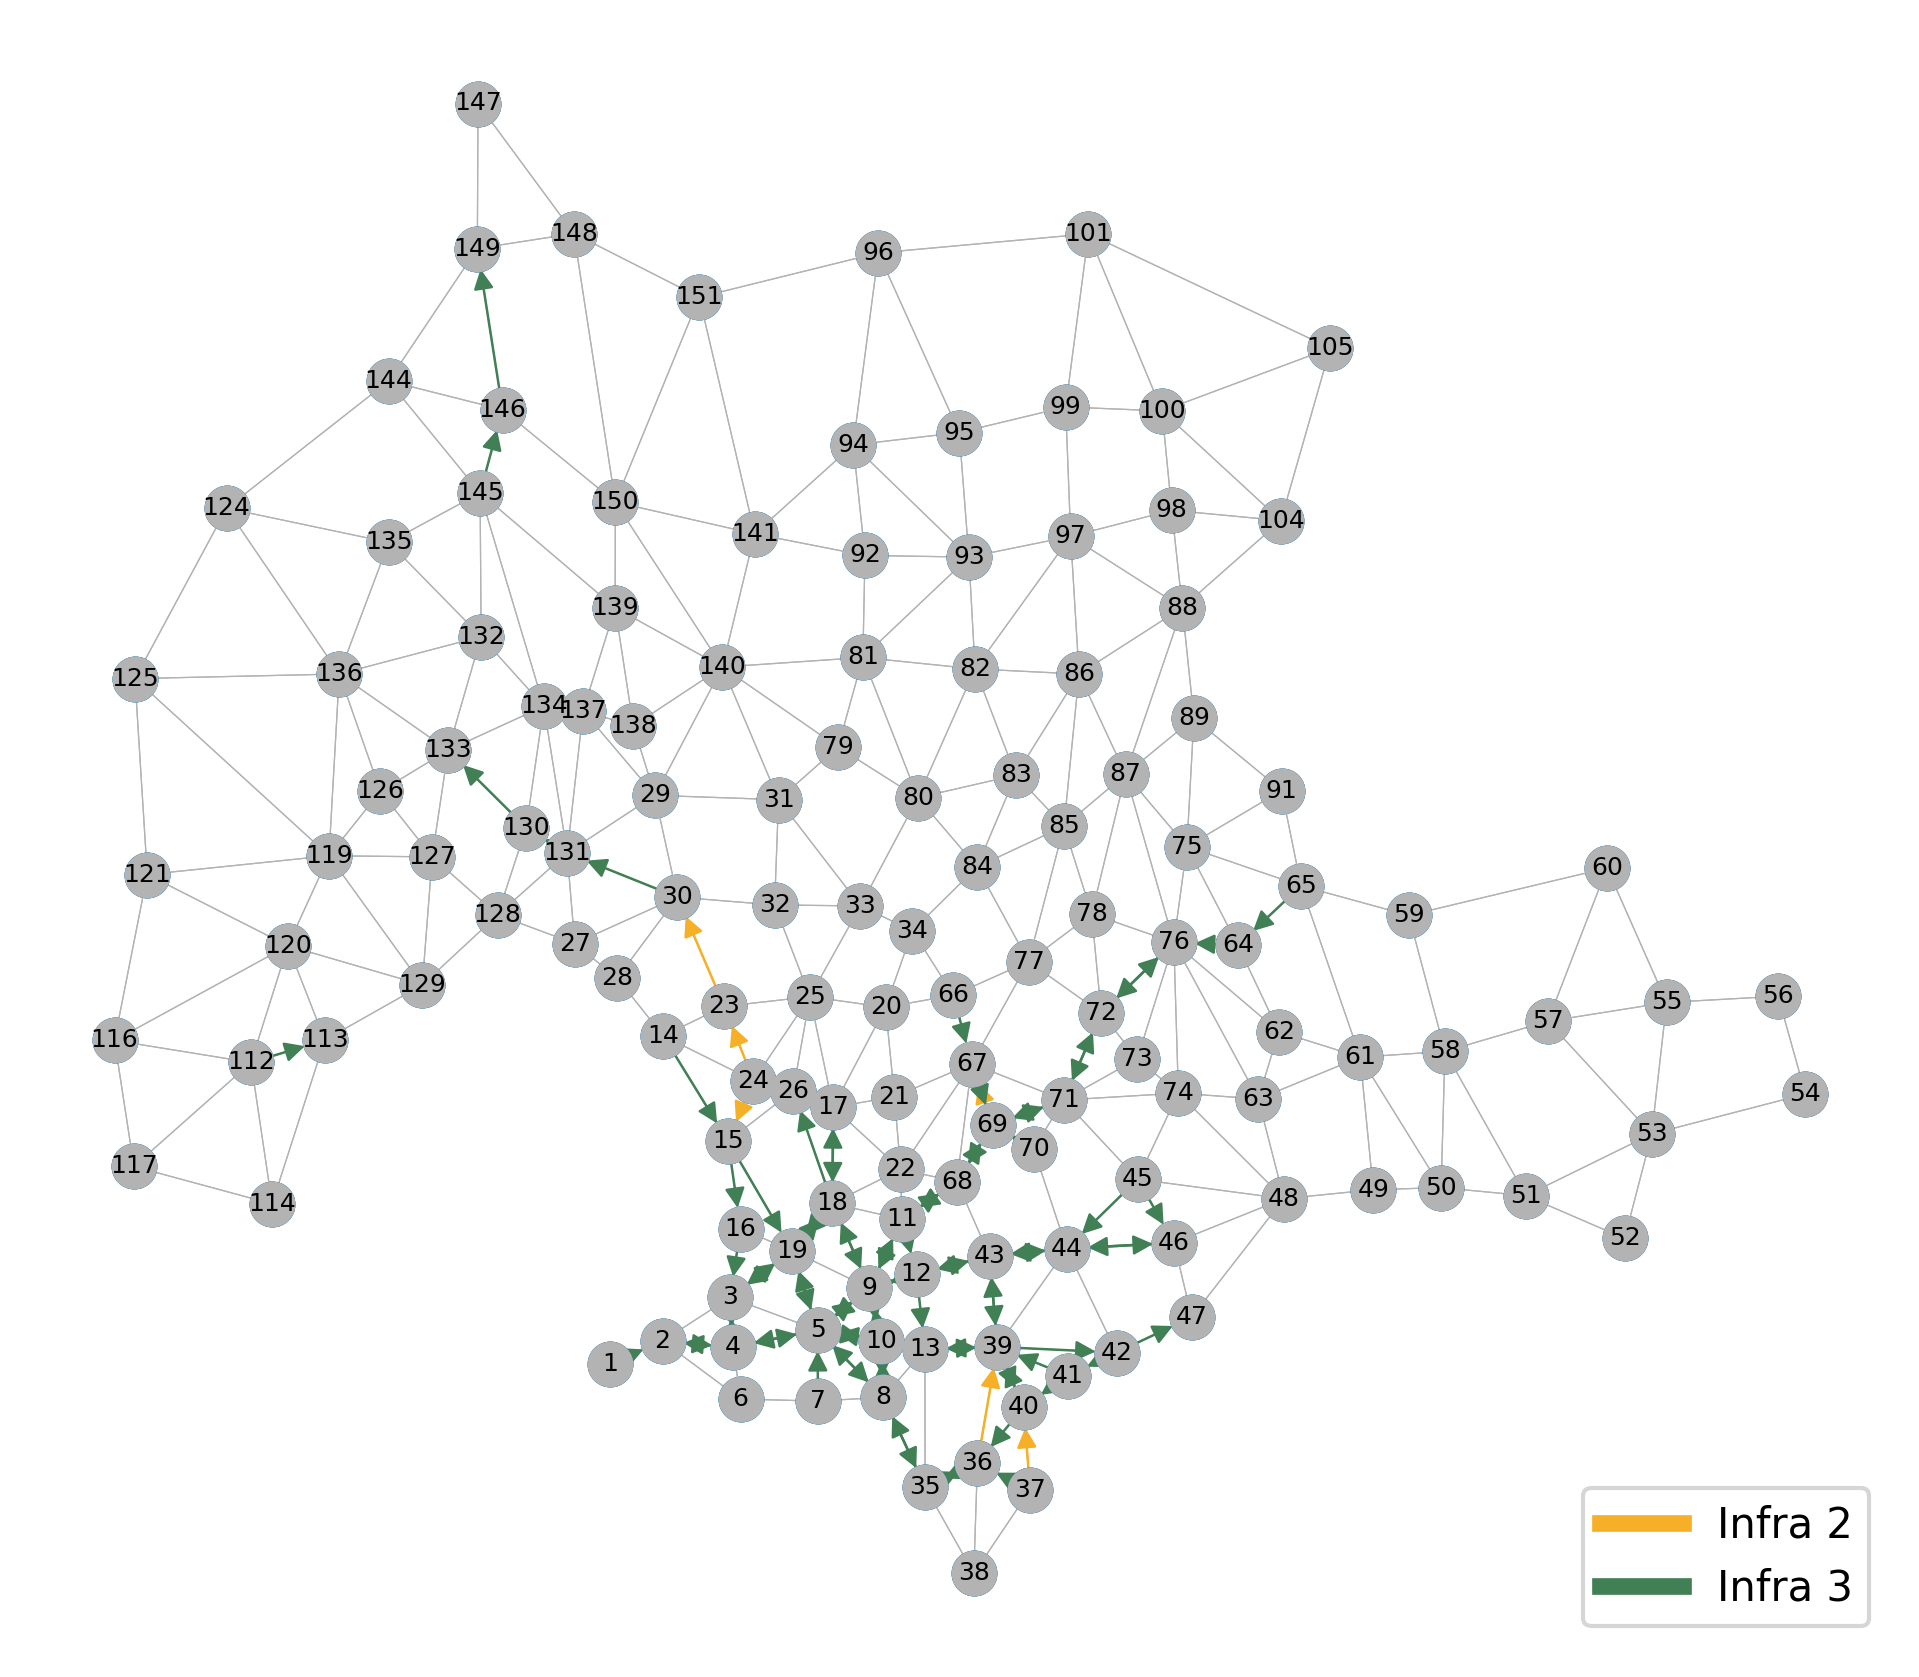
\includegraphics[width=6cm]{../resources/montevideo_d5000.0_inv_logit_0.4_budget_factor.png}
    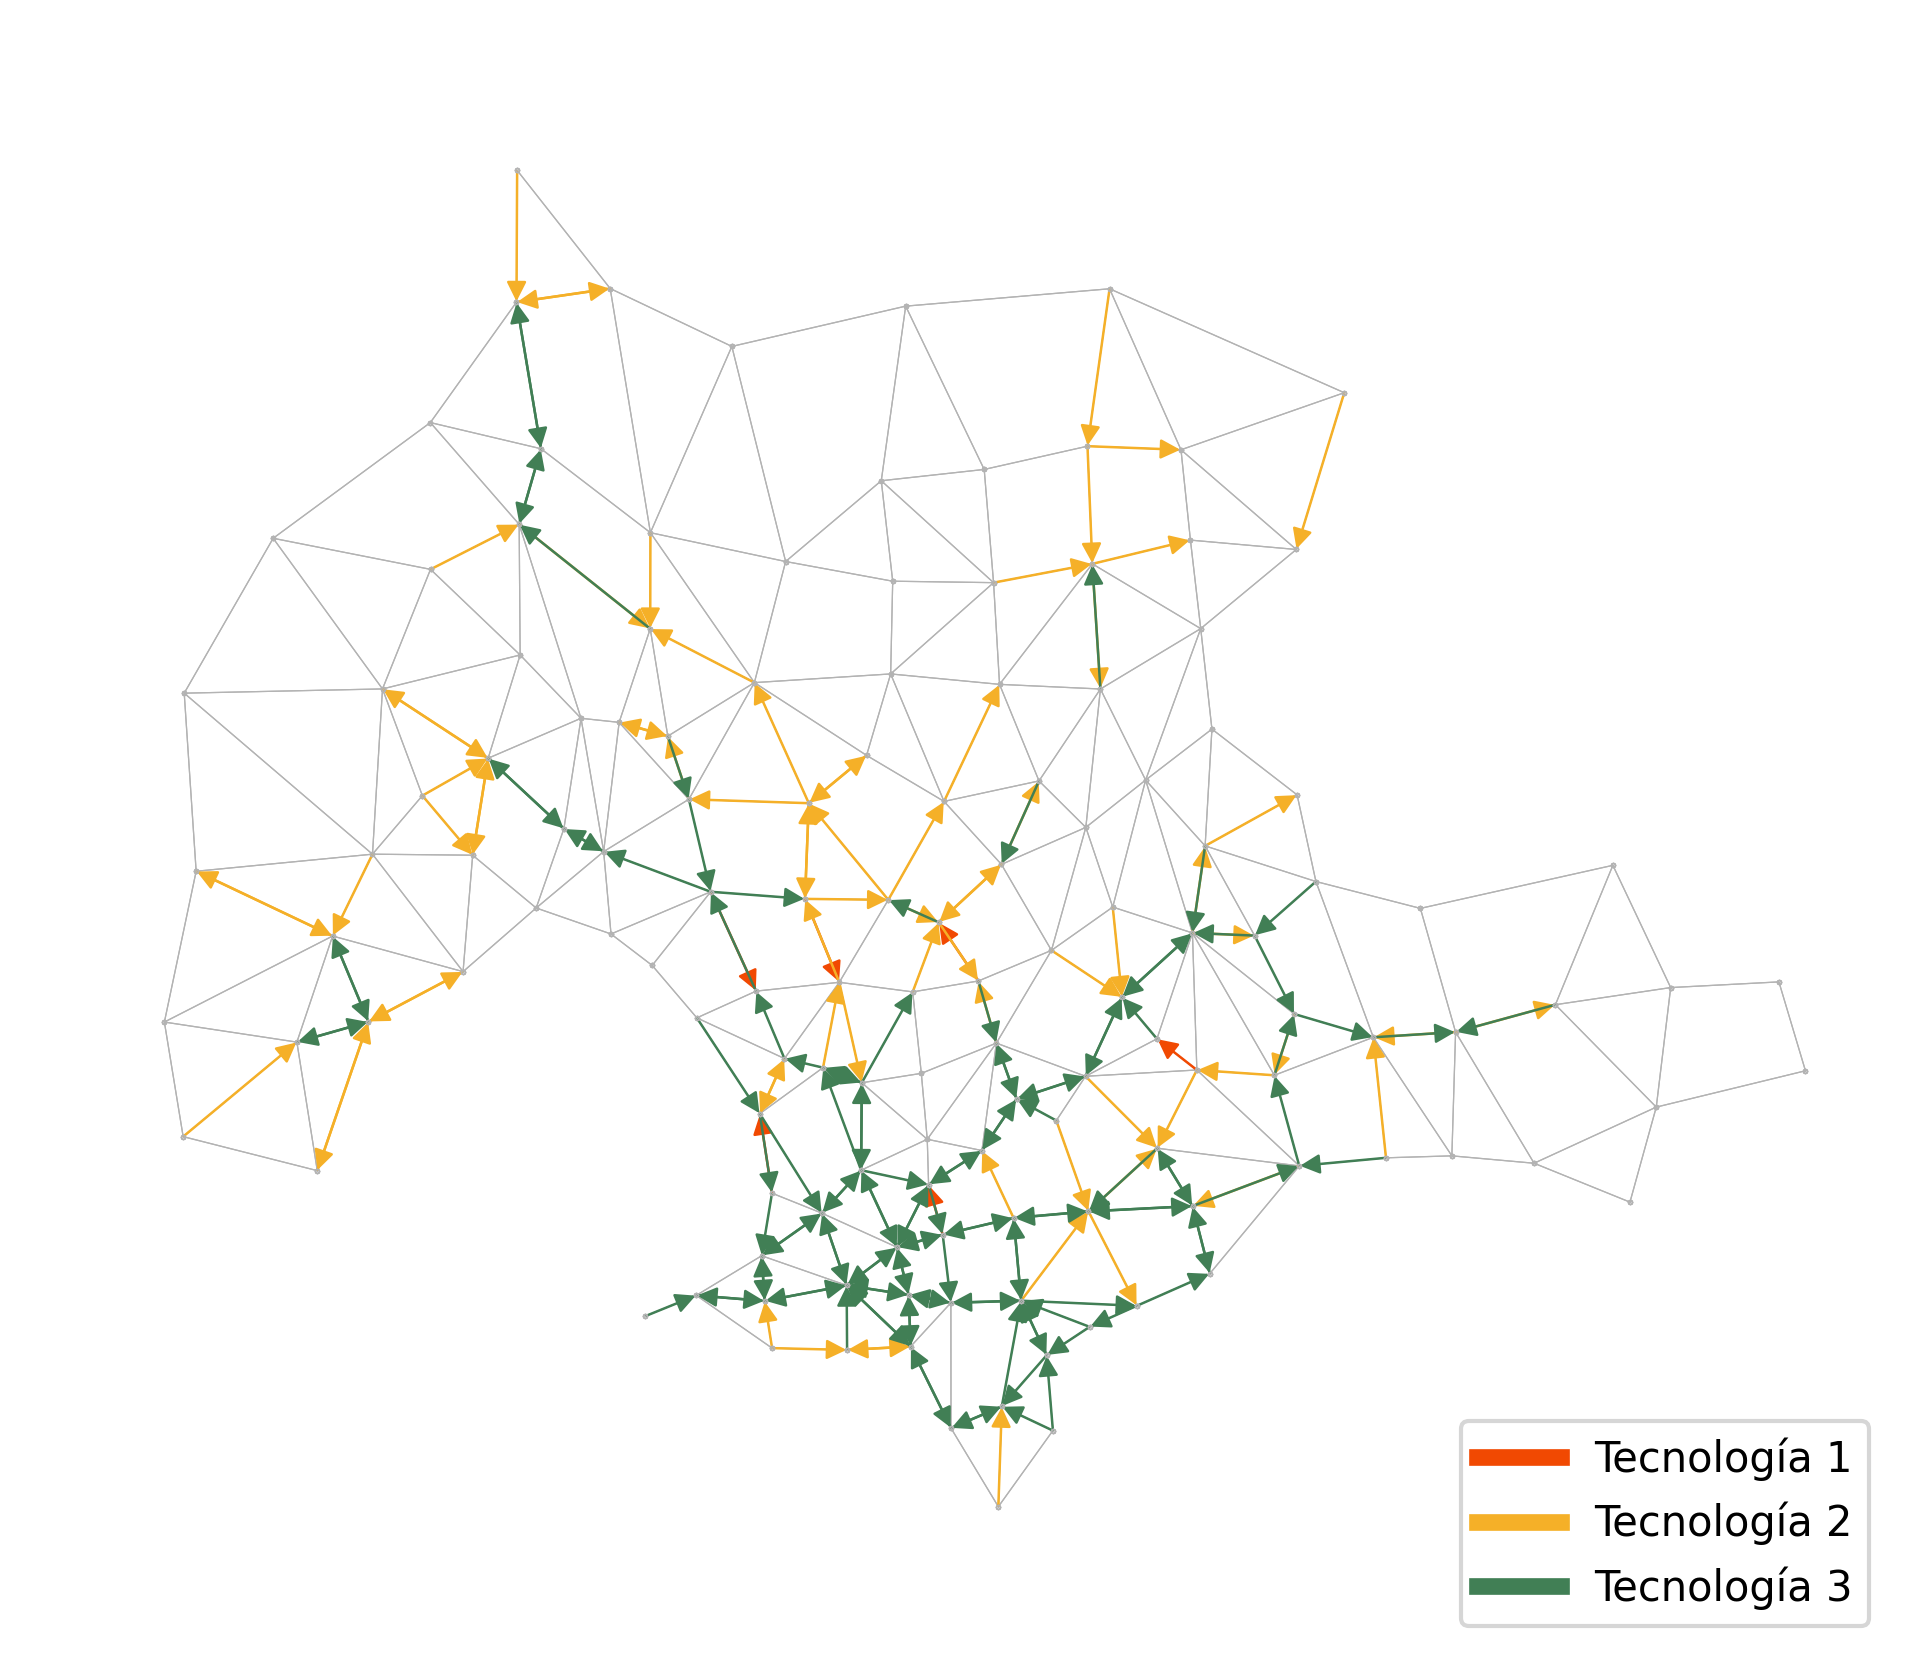
\includegraphics[width=6cm]{../resources/montevideo_d5000.0_linear.png}
    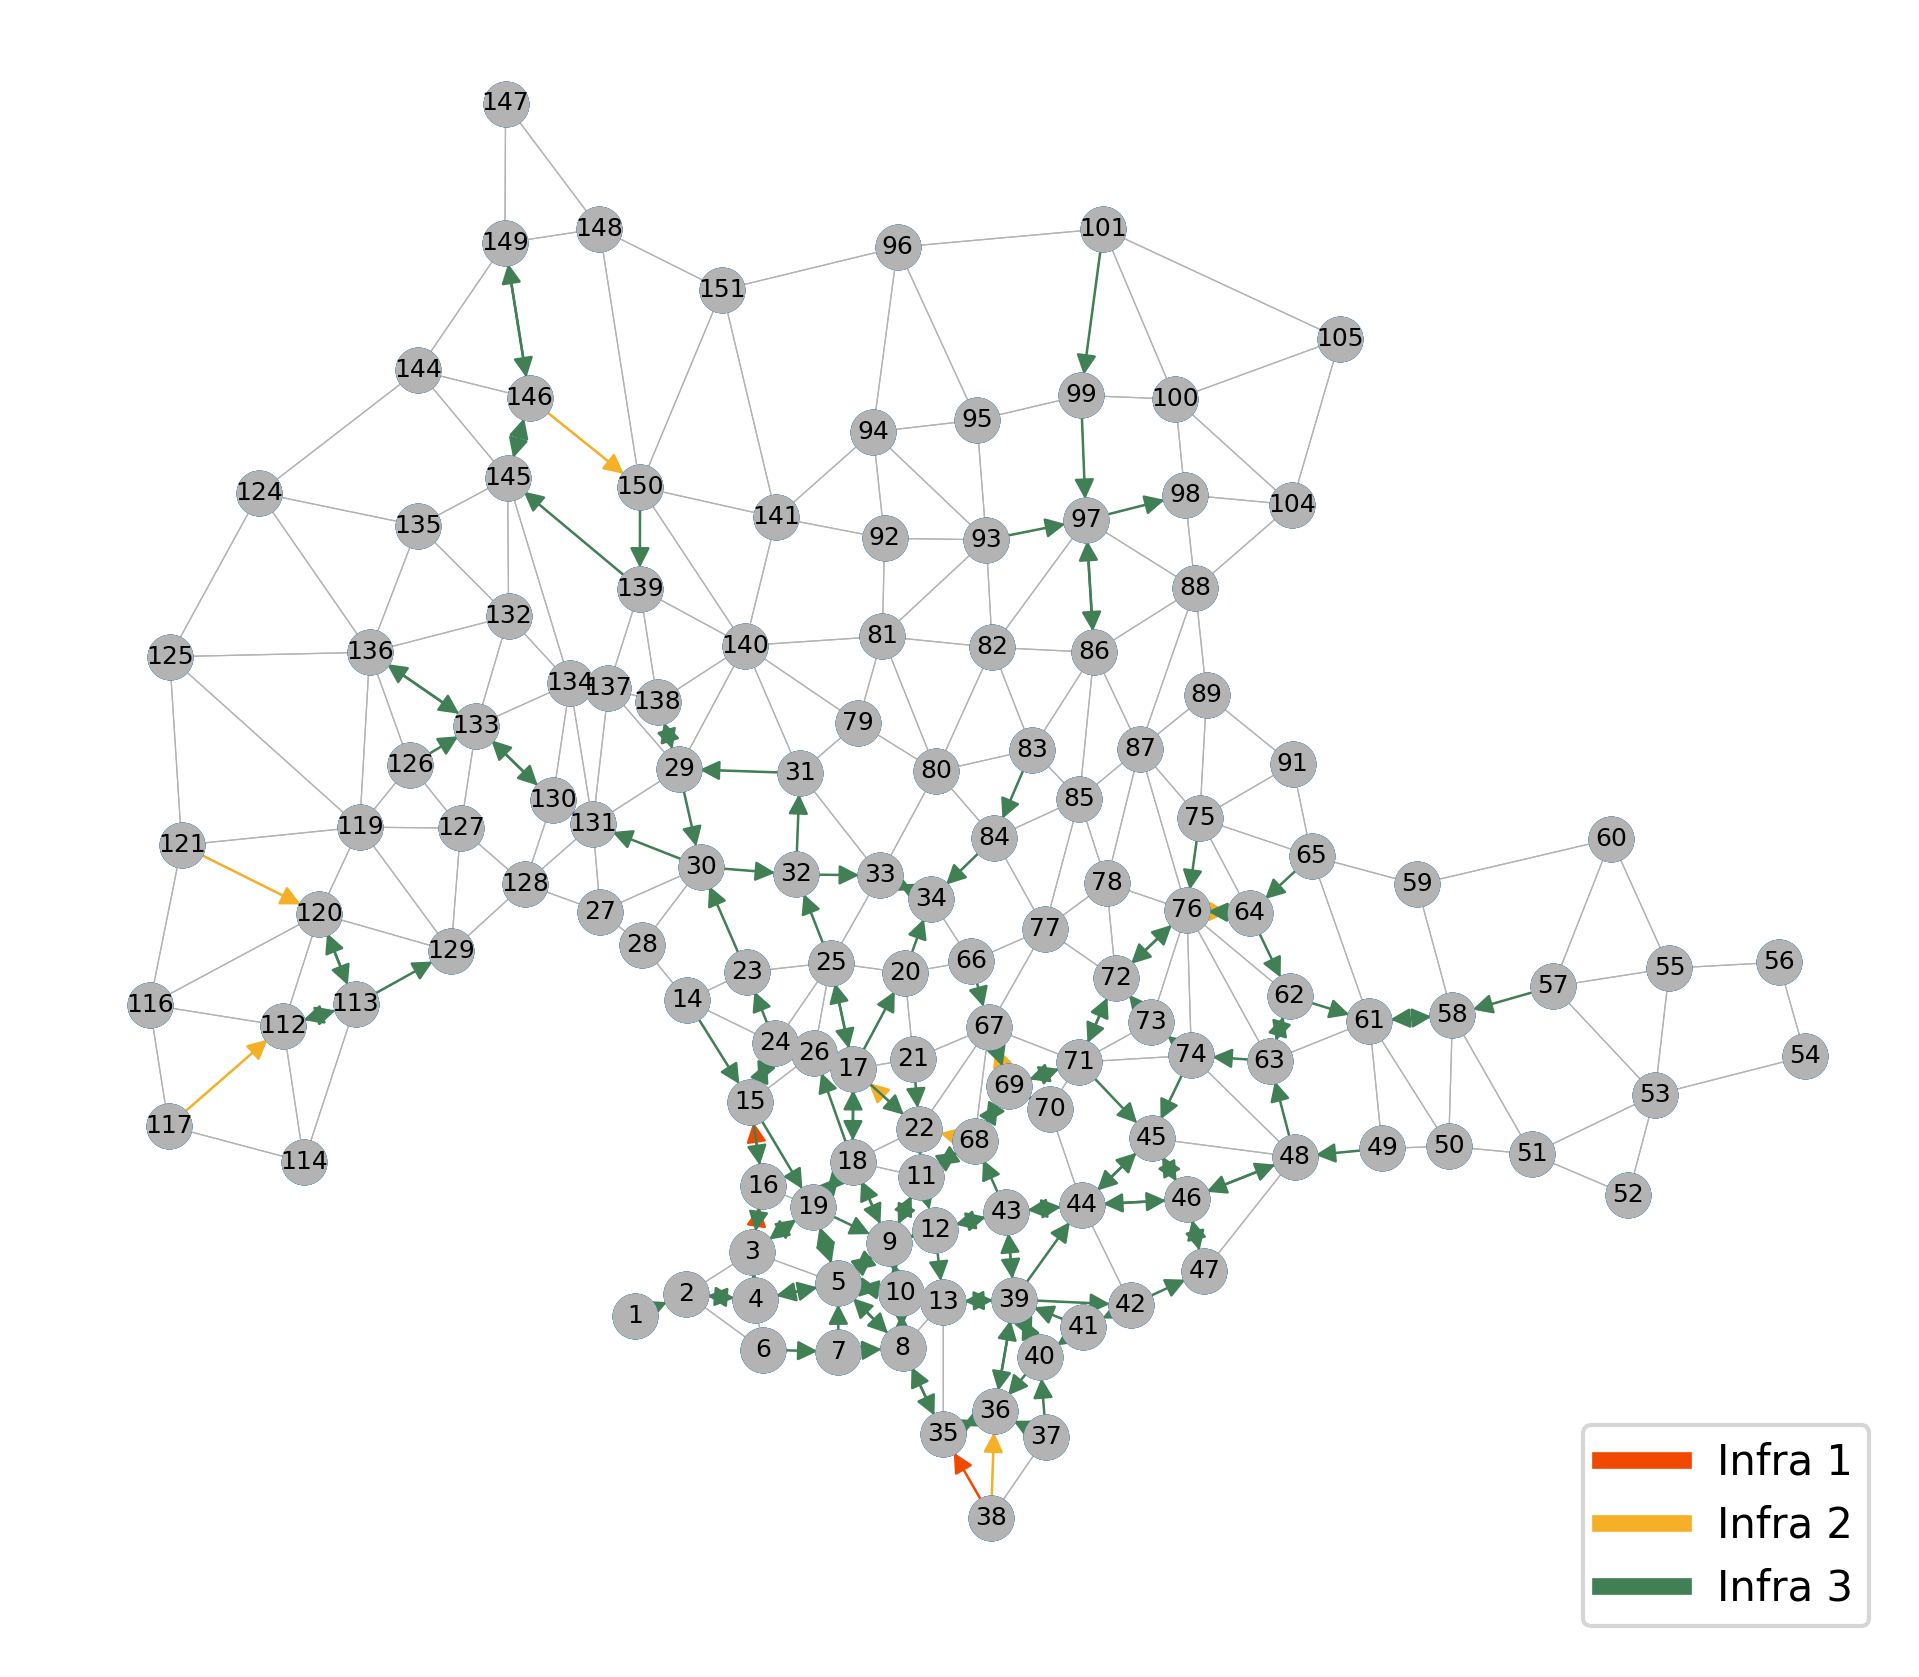
\includegraphics[width=6cm]{../resources/montevideo_d5000.0_inv_logit.png}
    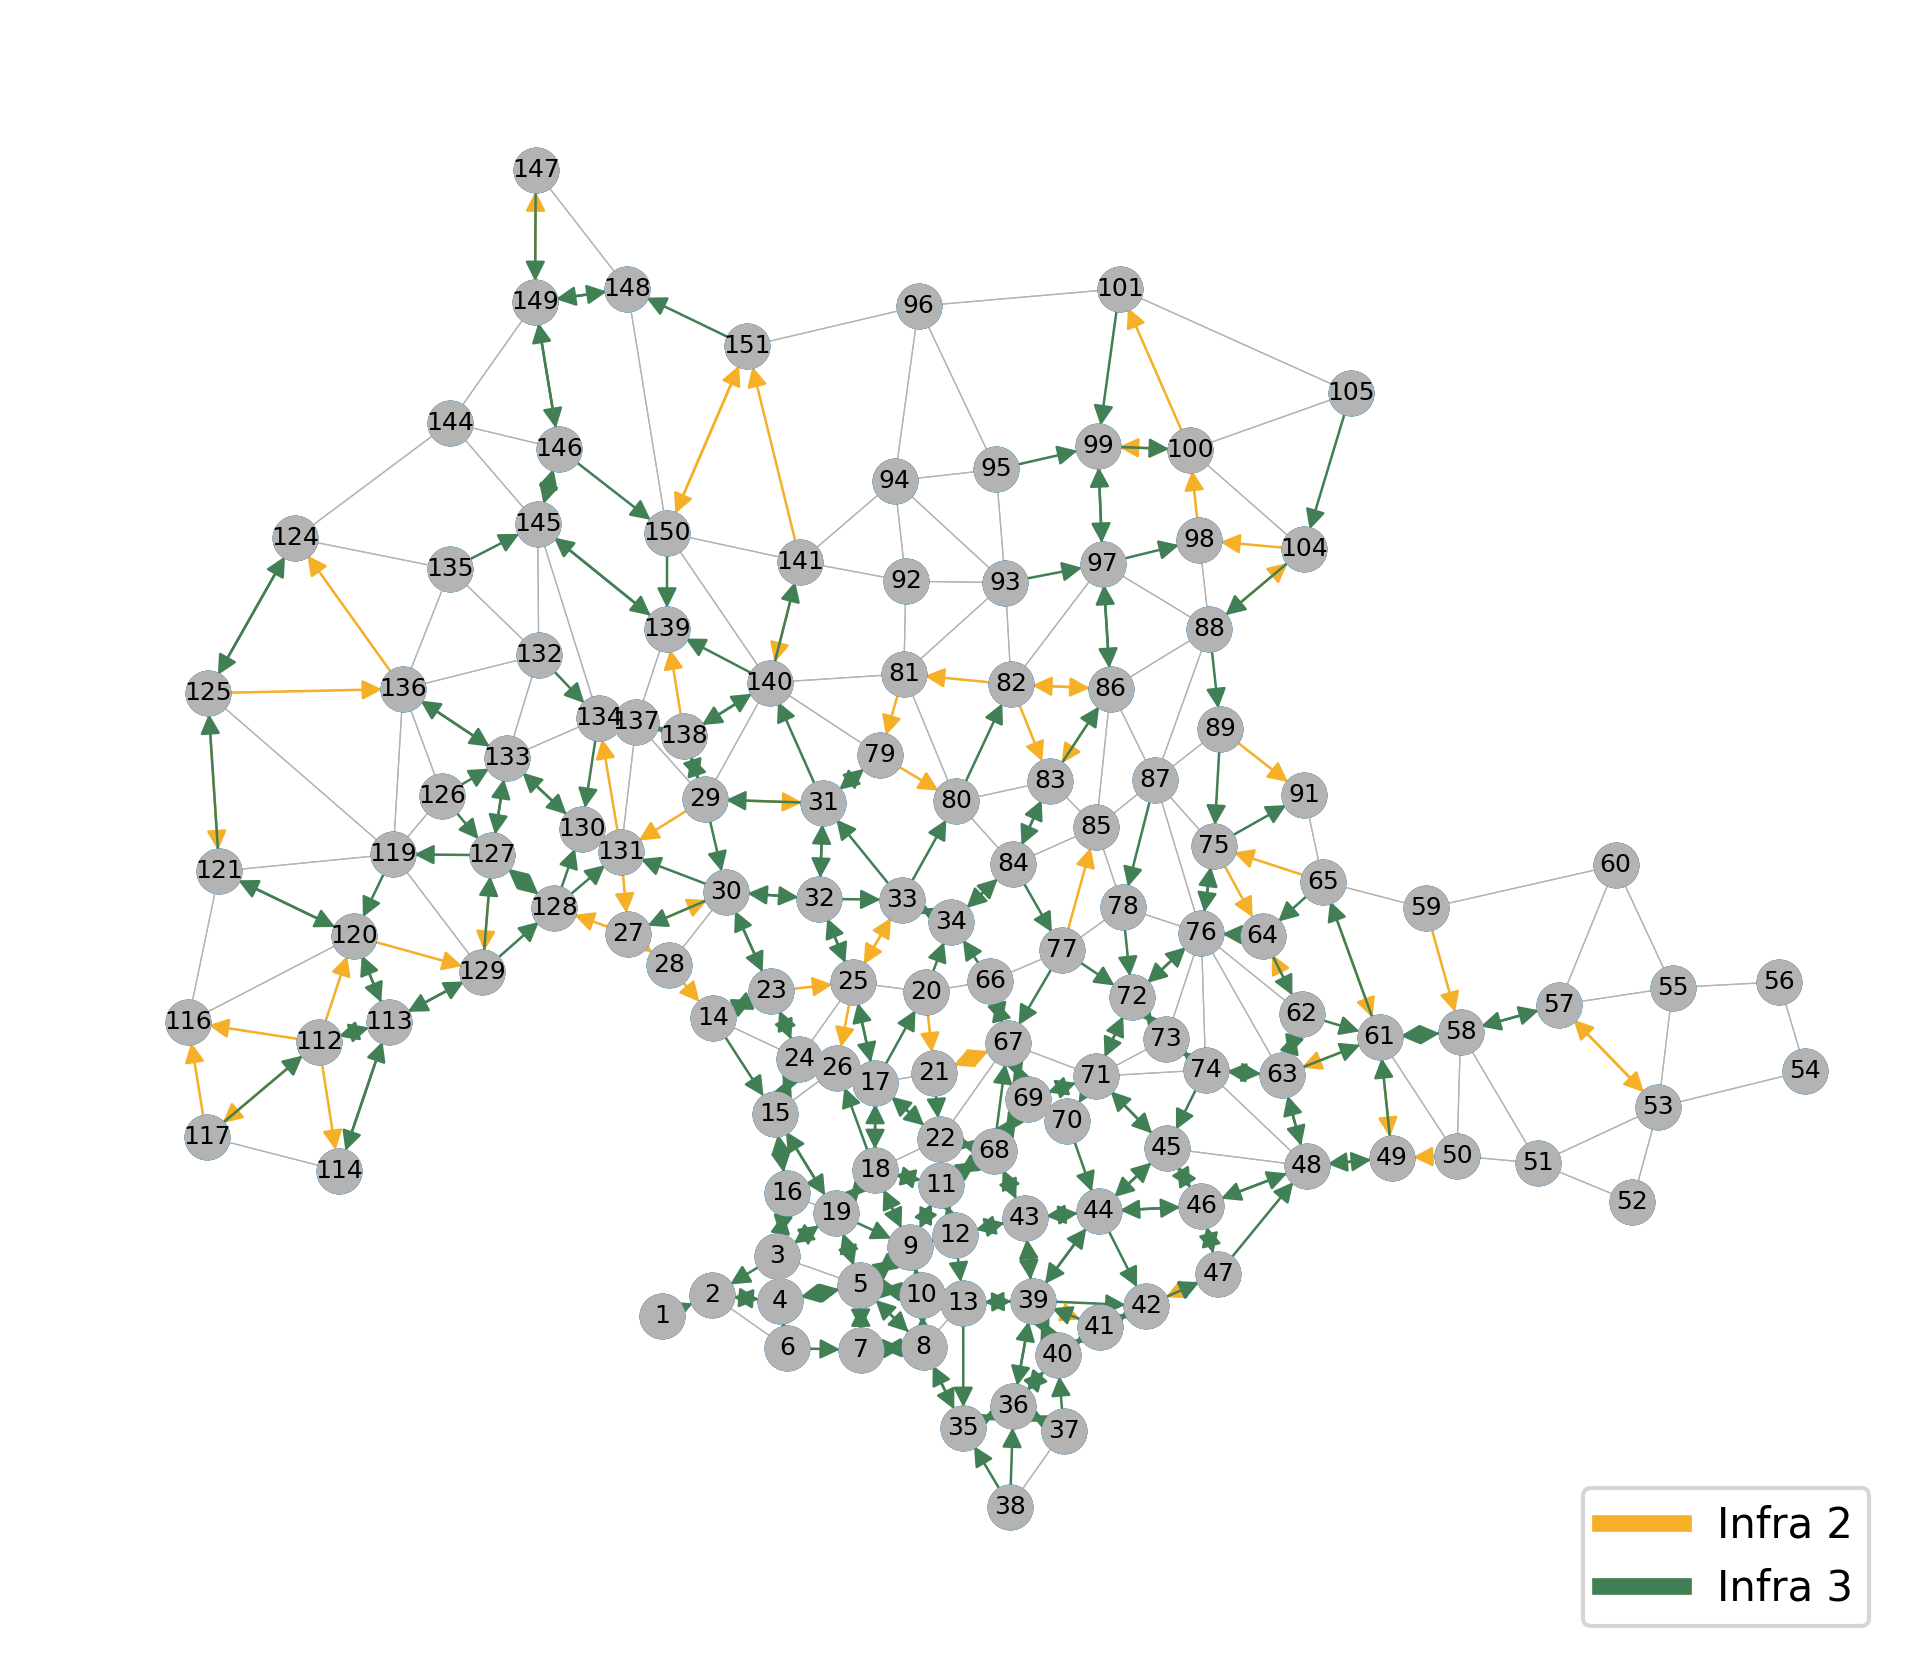
\includegraphics[width=6cm]{../resources/montevideo_d5000.0_linear_1.6_budget_factor.png}
    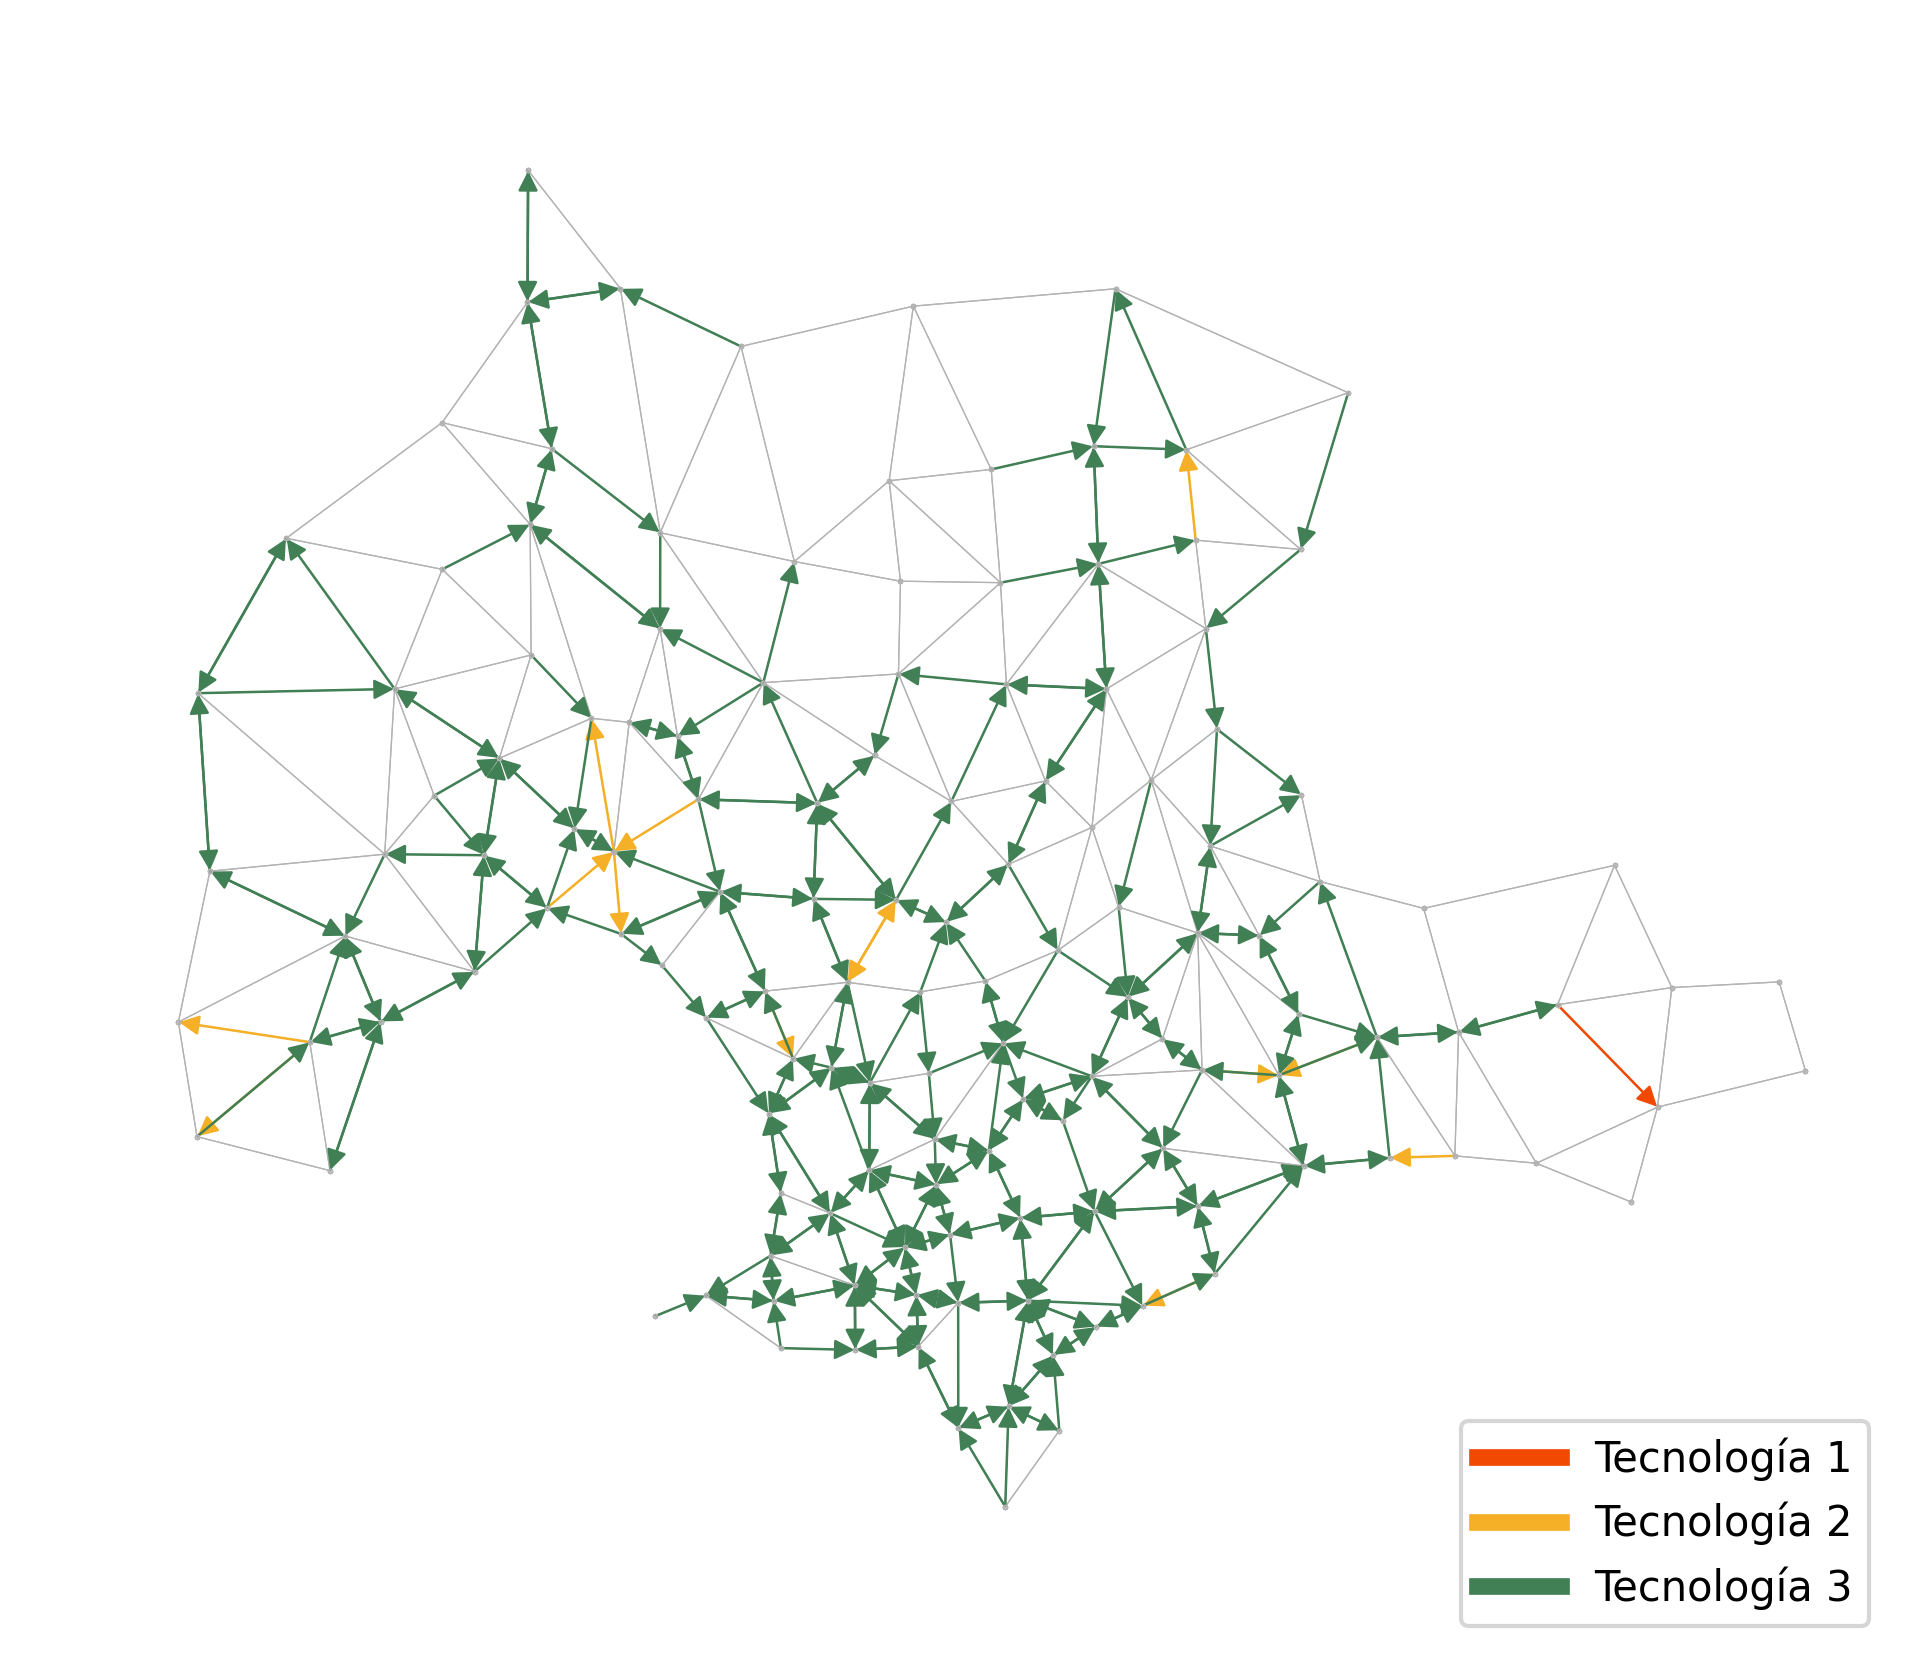
\includegraphics[width=6cm]{../resources/montevideo_d5000.0_inv_logit_1.6_budget_factor.png}
    \caption{Infraestructuras construidas para cada instancia. A la izquierda se ubican aquellas con función de transferencia de demanda lineal, a la derecha las que utilizan función logística. Además están dispuestas en orden creciente de factor de presupuesto desde arriba.}
    \label{fig:montevideo_instances_infras}
  \end{figure}

  \section{Conclusiones y trabajo a futuro}

  En este trabajo proponemos un enfoque alternativo al problema de diseño de ciclovías. Consideramos varios tipos de infraestructuras y permitimos modelar el comportamiento de la demanda de manera que pueda adaptarse a diferentes realidades. Esta última característica es la principal diferencia con trabajos anteriores y puede ser considerado el principal aporte a la comunidad académica.

  Mediante la realización de experimentos numéricos en una instancia chica y una que representa a una ciudad de medio tamaño mostramos que es posible construir una red de ciclovías que influye en buena medida la demanda cubierta incluso con lo que se considera bajos factores de presupuesto.

  A futuro, identificamos algunos caminos de trabajo. En primer lugar, extender la formulación propuesta en este trabajo para que considere otros aspectos manejados en otros trabajos como discontinuidades en los tipos de infraestructura, como en \cite{baya2021}, integrar el concepto de camino seguro, de \cite{lim2021}, y permitir distinguir qué tipos de infraestructura se puede construir en cada arco de la red que puede ser necesario para contemplar las diferentes realidades dentro de una ciudad.

  También se podría adaptar el modelo a un enfoque de bicicletas compartidas, realidad que es común en otras partes del mundo y requiere tener en cuenta los centros de estacionamientos requeridos para este tipo de bicicletas.

  Entendemos que seguir agregando complejidad al modelo puede resultar en que sea inaplicable debido a los altos tiempos de ejecución dado que en la situación actual ya nos encontramos con un límite en el generoso hardware con el que dispusimos. Identificamos dos alternativas para circunvalar esta situación: se pueden analizar dos alternativas: solucionar el problema de manera aproximada con una metaheurística ó reestructurar el problema y utilizar descomposición de Benders específica como se implementó en \cite{lim2021} con resultados muy buenos.

  Respecto a los datos, en este trabajo estimamos y aproximamos muchos de los parámetros. Pensamos que puede ser interesante aplicar este problema con datos más realistas. Luego podemos comparar las soluciones del modelo en términos de demanda transferida contra la vida real de dos formas: la más costosa sería mediante encuestas suponiendo que ciertas infraestructuras son construidas, la otra sería contrastar los resultados del modelo contra ciudades que mantengan algún histórico de datos de utilización de la bicicleta y cobertura de ciclovías.

  \newpage
  \section{Apéndices}

  \subsection{Validación de la formulación binivel}
  \label{sect:apendixbilevelvalidation}

  Para discutir la validez matemática del modelado binivel (\ref{eq:objective1lvl})-(\ref{eq:flowbalance}) partimos de una formulación estándar de problema binivel o BLPP (Bi Level Programming Problem), como se puede encontrar en Bard \cite{bardbook} y demostramos la validez en base a las definiciones ahi mencionadas.
  Sea la siguiente formulación simplificada del problema:

  \begin{align}
    \text{max}_{y \in Y}    & \; F(x, y) \label{bilevelgeneric1} \\
    \text{s.t.} \modelspace & A_1 x + B_1 y \leq b_1 \\
                            & y \geq 0 \\
                            & \text{min}_{x \in X} f(x, y) \\
                            & \modelspace A_2 x + B_2 y \leq b_2 \label{bilevelgeneric5} \\
                            & \modelspace x \geq 0 \label{bilevelgeneric6}
  \end{align}

  Y las siguientes definiciones:

  \begin{definition}
    Conjunto factible
    \begin{align}
      S = \{(x, y) \setminus x \in X, y \in Y, A_1 x + B_1 y \leq b_1, A_2 x + B_2 y \leq b_2 \}
    \end{align}
  \end{definition}

  \begin{definition}
    Conjunto de reacción del segundo nivel:
    \begin{align}
      P(y) = \{ x \in \text{argmin}_{\hat{x} \in X} f(\hat{x}, y) : A_2 \hat{x} + B_2 y \leq b_2 \}
    \end{align}
  \end{definition}

  Diremos que el problema está bien formulado si el conjunto $S$ es no vacío, es decir, si existen soluciones factibles y si para toda $y$ el conjunto $P(y)$ es no vacío, en otras palabras, si para todo movimiento del problema de primer nivel, hay margen de decisión en el segundo nivel.

  \begin{lemma}$S$ es no vacío
  \end{lemma}

  \begin{proof}
    $S \neq \emptyset$ ya que $\exists (x_0, y_0) \in X \times Y$ donde $y_0$ es el vector $y_{ai_0} = 1 \forall a \in A$, $i_0$ es la infraestructura cuyo costo $H_{ai_0} = 0$, lo que deja al resto de las entradas del vector $y_0$ en $0$. Por lo tanto se cumple la restricción (\ref{eq:alwaysoney}) dado que todos los arcos tienen una infraestructura activa, y la restricción (\ref{eq:respectbudget}) dado que el costo total de construcción de $y_0$ es $0$.

    Luego, dado que las infraestructuras activas logran la conectividad de los pares origen-destino y el hecho de que el costo de los arcos $C_ai$ sea no negativo, posibilita asegurar que el problema de segundo nivel tiene al menos una solución factible $x_0$.
  \end{proof}

  \begin{lemma}$\forall y \in Y,\; P(y) \neq \emptyset$
  \end{lemma}

  \begin{proof}
    Para cualquier asignación $y = \hat{y} \in Y$, se cumple que $P(\hat{y})$ es no vacío ya que todos los arcos tienen una infraestructura activa, por lo tanto el grafo donde los flujos del problema de segundo nivel pueden pasar es conexo y llega necesariamente a todos los nodos, incluyendo los pares origen-destino. Por lo tanto el espacio de soluciones factibles del subproblema es no vacío. 
  \end{proof}

  Aún cuando estas dos definiciones se cumplen, pueden haber dificultades al encontrar la solución óptima cuando $P(y)$ contiene más de un elemento, caso en el cual el modelo puede no llegar a la solución óptima dependiendo del valor $x \in P(y)$ que seleccione el problema de segundo nivel. En este caso de estudio es muy probable que esto suceda, puesto que pueden haber varios caminos más cortos entre dos puntos.
  % TODO: Aquí entran en juego las definiciones de enfoque pesimista y optimista. Sería bueno discutir cual de los dos se adopta en este trabajo. En general esto queda determinado por el método de resolución.

  \subsection{Transformación por condiciones de KKT}
  \label{sec:kkttransform}

  Sea la formulación genérica binivel (\ref{bilevelgeneric1})-(\ref{bilevelgeneric6}), y sea $f(x, y) = cx + dy$, entonces podemos sustituir el problema de segundo nivel por sus condiciones de optimalidad de KKT agregando las variables $v$ y $u$ de la siguiente manera:

  \begin{align}
    \text{max}_{x,y}        & \; F(x, y) \label{kktgeneric1} \\
    \text{s.t.}             & A_1 x + B_1 y \leq b_1 \\
                            & uA_2 - v = -c \\
                            & u(b_2 - A_2x - B_2y) + vx = 0 \label{kktgeneric_complslack} \\
                            & A_2 x + B_2 y \leq b_2 \label{kktgeneric5} \\
                            & x, y, v, u \geq 0 \label{kktgeneric6}
  \end{align}

  La restricción (\ref{kktgeneric_complslack}) es problemática dado que el objetivo es resolver el problema con un solver lineal. Aplicando el teorema de holgura complementaria sabemos que ambos sumandos son 0. Luego, podemos reemplazar la restricción $u(b_2 - A_2x - B_2y) = 0$ por dos conjuntos de restricciones equivalentes, agregando variables binarias $z$ y una constante $M$ suficientemente grande, de manera que quede: $u \leq Mz$ y $b_2 - A_2x - B_2y \leq M(1-z)$.

  Si aplicamos esta transformación a nuestro problema binivel tendríamos que agregar $|N| |OD|$ variables binarias. Considerando las ya existentes variables $y_{ai}$ y las que agregaremos por temas intrínsecos del problema, entendemos que esto supone una complejidad que supera a la formulación implementada.

  \subsection{Detalles de implementación}

  Durante el transcurso del proyecto desarrollamos una pequeña biblioteca escrita en Python \footnote{\url{https://gitlab.fing.edu.uy/joaquin.correa/bicycle-network-design}} que facilita la manipulación y especificación de datos y la ejecución de las diferentes formulaciones sobre diferentes solvers. Esto permitió simplificar la tarea de ejecución y manipulación de parámetros significativamente, por ejemplo alterar los parámetros de una instancia como la red subyacente o la demanda, generar instancias aleatorias sobre una red o aplicar el problema sobre grafos obtenidos de OpenStreeMaps \footnote{\url{https://www.openstreetmap.org/}}. Especificamos un formato de salida unificado que simplificó el análisis de las soluciones por medio del parseo de los archivos de solución de los solvers. Esto nos permitió la rápida comparativa de un gran volumen de soluciones así como la representación gráfica de los resultados.

  La formulación del problema la escribimos en el lenguaje GNU MathProg \footnote{\url{https://lpsolve.sourceforge.net/5.5/MathProg.htm}} debido a su simpleza y expresividad. Utilizamos tres solvers durante el proyecto: GLPK \footnote{GNU Linear Programming Kit}, CBC \footnote{\ Coin-or branch and cut MIP solver} y AMPL/CPLEX \footnote{IBM CPLEX Optimizer}. Los primeros dos son libres y de código abierto y fueron utilizados en las primeras etapas del proyecto. GLPK fue tomado como punto de partida y referencia debido a su estabilidad y utilización en el área. CBC demostró ser más rápido que GLPK gracias a que saca provecho de procesamiento paralelo, pero su utilización fue, subjetivamente, ligeramente más complicada debido a que requiere compilación manual con la extensión de GNU MathProg y en su salida no notifica cuando una instancia del problema es no factible. Luego, pagamos el precio de la necesidad de abandonar las soluciones de código libre para bajar los tiempos de ejecución sobre instancias más complejas y utilizamos AMPL/CPLEX para ejecutar las pruebas de las secciones de análisis de sensibilidad y aplicación sobre una instancia realista.

  \subsubsection{Datos de la red}
  \label{sect:costcalculation}

  Las redes utilizadas deben tener una serie de datos asociados de manera que sea posible solucionarlas con el software desarrollado. Para los nodos es necesario (no estrictamente) tener su par de coordenadas. Para los arcos, se necesitan los siguientes atributos:

  \begin{description}
    \item[user\_cost (abreviado CU)]: Costo de usuario de atravesar el arco sobre el grafo base (sin infraestructura o con la infraestructura base $i_0$).
    \item[construction\_cost (abreviado CC)]: Costo de construcción de la infraestructura 1.
  \end{description}

  Luego, si se tienen las infraestructuras $I = \{1, 2, 3, ... \}$, para la infraestructura $i$ se calcula el costo de usuario de atravesarla como $CU_i = {28 - 3 (i + 1) \over 25}$. El valor del costo de construcción será $CC_i = 2i CC$. De ser necesario, pueden especificarse valores particulares de costos de dicha infraestructura para un arco determinado mediante la utilización de los atributos $user\_cost\_i$ y $construction\_cost\_i$.

  \subsection{Especificación de funciones de transferencia de demanda}

  Las funciones de transferencia de demanda probadas fueron cuatro, ver figura (\ref{fig:fcatalog}). Las cuatro funciones se definen parametrizadas por $m$, correspondiente a la proporción de mejora máxima alcanzable por la mejor infraestructura, es decir $m = min_{i \in I - \{0\}} \{ C_{infra}(i) \}$. Definimos entonces las funciones en $[m, 1] \rightarrow [0, 1]$ de la siguiente manera:

  \begin{definition}
    Lineal
    \begin{align}
        f(x) = {x -1 \over m - 1}
    \end{align}
  \end{definition}

  \begin{definition}
    Logística
    \begin{align}
        f(x) = {1 \over 1 + e^{2k_m(x - ({1 + m \over 2}))}}
    \end{align}
  \end{definition}

  \begin{definition}
    Concavidad negativa: logística entre $[m, 1)$
    \begin{align}
        f(x) = {2 \over 1 + e^{k_m(x - 1)}} - 1
    \end{align}
  \end{definition}

  \begin{definition}
    Concavidad positiva: logística entre $[m, 1)$
    \begin{align}
        f(x) = {2 \over 1 + e^{k_m(x - m)}}
    \end{align}
  \end{definition}

  El parámetro $k_m$ determina la cuesta de las funciones logísticas y es utilizado para que los valores funcionales en los extremos de $(m, 1)$ estén cerca de $1$ y $0$ respectivamente. Fue determinado de manera experimental y se calcula como $k_m = {3 \over 1 - m}$

  \subsection{Instancia de Sioux-Falls}

  Esta instancia se utilizó para las pruebas preliminares y de sensibilidad de parámetros. Aquí se especifican los datos del grafo, costos de usuario sobre la infraestructura base, de construcción en la tabla (\ref{table:siouxfallsgraphdata}) y datos de demanda (\ref{table:siouxfallsdemanddata}). La representación se puede observar en la figura (\ref{fig:siouxfallsapendix}).

  \begin{figure}[h!]
    \centering
    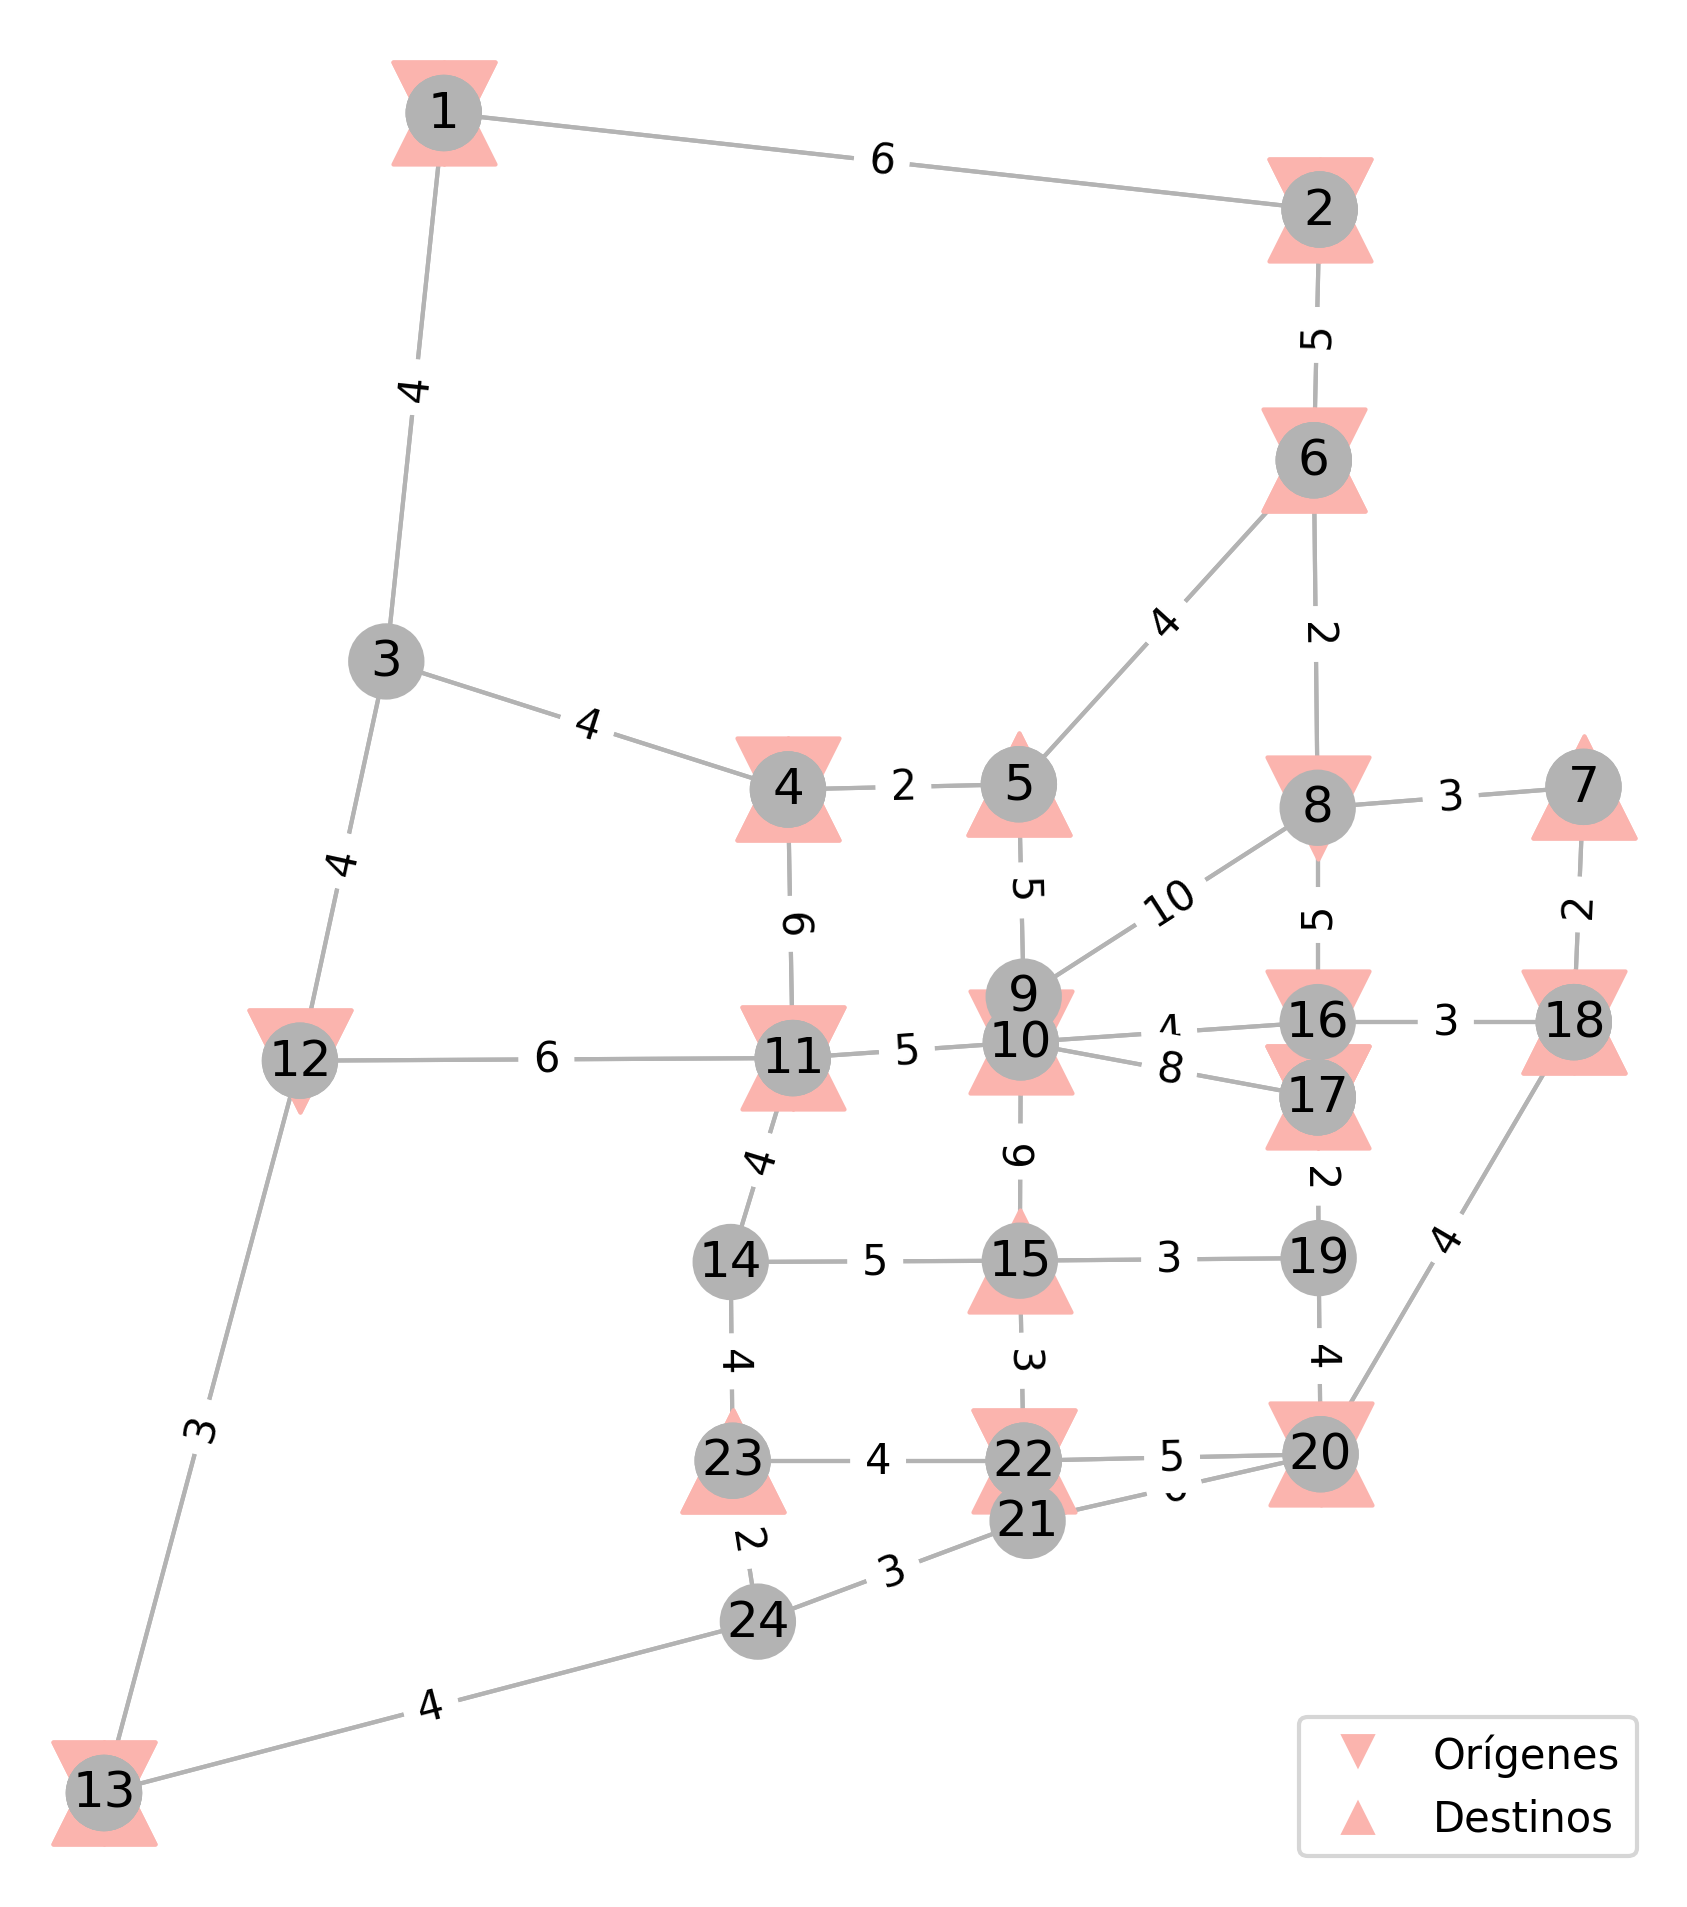
\includegraphics[width=8cm]{../resources/sioux_falls_odpairs.png}
    \caption{Representación de la red de la instancia de Sioux-Falls.}
    \label{fig:siouxfallsapendix}
  \end{figure}

  \begin{table}[h!]
    \centering
    \caption*{{\bf Costo de arcos de la instancia de Sioux-Falls}}
    \begin{tabular}{ccc}
      \toprule
        Arco & Costo \\
      \midrule
        (1, 2) & 6 \\
        (1, 3) & 4 \\
        (2, 1) & 6 \\
        (2, 6) & 5 \\
        (3, 1) & 4 \\
        (3, 4) & 4 \\
        (3, 12) & 4 \\
        (4, 3) & 4 \\
        (4, 5) & 2 \\
        (4, 11) & 6 \\
        (5, 4) & 2 \\
        (5, 6) & 4 \\
        (5, 9) & 5 \\
        (6, 2) & 5 \\
        (6, 5) & 4 \\
        (6, 8) & 2 \\
        (7, 8) & 3 \\
        (7, 18) & 2 \\
        (8, 6) & 2 \\
        (8, 7) & 3 \\
        (8, 9) & 10 \\
        (8, 16) & 5 \\
        (9, 5) & 5 \\
        (9, 8) & 10 \\
        (9, 10) & 3 \\
        (10, 9) & 3 \\
      \bottomrule
    \end{tabular}
    \begin{tabular}{ccc}
      \toprule
        Arco & Costo \\
      \midrule
        (10, 11) & 5 \\
        (10, 15) & 6 \\
        (10, 16) & 4 \\
        (10, 17) & 8 \\
        (11, 4) & 6 \\
        (11, 10) & 5 \\
        (11, 12) & 6 \\
        (11, 14) & 4 \\
        (12, 3) & 4 \\
        (12, 11) & 6 \\
        (12, 13) & 3 \\
        (13, 12) & 3 \\
        (13, 24) & 4 \\
        (14, 11) & 4 \\
        (14, 15) & 5 \\
        (14, 23) & 4 \\
        (15, 10) & 6 \\
        (15, 14) & 5 \\
        (15, 19) & 3 \\
        (15, 22) & 3 \\
        (16, 8) & 5 \\
        (16, 10) & 4 \\
        (16, 17) & 2 \\
        (16, 18) & 3 \\
        (17, 10) & 8 \\
        (17, 16) & 2 \\
     \bottomrule
    \end{tabular}
    \begin{tabular}{ccc}
      \toprule
        Arco & Costo \\
      \midrule
        (17, 19) & 2 \\
        (18, 7) & 2 \\
        (18, 16) & 3 \\
        (18, 20) & 4 \\
        (19, 15) & 3 \\
        (19, 17) & 2 \\
        (19, 20) & 4 \\
        (20, 18) & 4 \\
        (20, 19) & 4 \\
        (20, 21) & 6 \\
        (20, 22) & 5 \\
        (21, 20) & 6 \\
        (21, 22) & 2 \\
        (21, 24) & 3 \\
        (22, 15) & 3 \\
        (22, 20) & 5 \\
        (22, 21) & 2 \\
        (22, 23) & 4 \\
        (23, 14) & 4 \\
        (23, 22) & 4 \\
        (23, 24) & 2 \\
        (24, 13) & 4 \\
        (24, 21) & 3 \\
        (24, 23) & 2 \\
         & \\
         & \\
      \bottomrule
    \end{tabular}
    \caption{Costos de usuario y de construcción de la infraestructura 1 por arco de la red. Dado que utilizamos el largo del arco estos costos coinciden.}\label{table:siouxfallsgraphdata}
  \end{table}

  \begin{table}[h!]
    \centering
    \caption*{{\bf Pares origen-destino de la instancia de Sioux-Falls}}
    \begin{tabular}{ccc}
      \toprule
        Origen & Destino & Demanda \\
      \midrule
        1 & 7 & 34 \\
        1 & 23 & 3 \\
        2 & 13 & 6 \\
        2 & 17 & 4 \\
        4 & 11 & 9 \\
        6 & 1 & 14 \\
        8 & 15 & 10 \\
        10 & 22 & 13 \\
        11 & 5 & 20 \\
        11 & 13 & 1 \\
        12 & 2 & 6 \\
        12 & 10 & 27 \\
        13 & 4 & 5 \\
        13 & 6 & 12 \\
        16 & 18 & 10 \\
        17 & 5 & 9 \\
        17 & 20 & 13 \\
        17 & 23 & 14 \\
        18 & 6 & 16 \\
        20 & 7 & 11 \\
        22 & 4 & 15 \\
        22 & 18 & 6 \\
      \bottomrule
    \end{tabular}
    \caption{Pares origen-destino utilizados para la red de Sioux-Falls con costos por arco.}\label{table:siouxfallsdemanddata}
  \end{table}

  \FloatBarrier
  \printbibliography
\end{document}
